\documentclass[11pt,english,a4paper]{article}
\usepackage{xifthen,iftex}
\ifluatex
\else
    \usepackage[utf8]{inputenc}% force UTF8 file encoding if no UTF8 engine is used
\fi
\usepackage[T1]{fontenc}% T1 font encoding
\usepackage[l2tabu,orthodox]{nag}
\usepackage{microtype}
\usepackage{etoolbox}
\usepackage{XCharter}% default font
\usepackage[uprightscript,charter,vvarbb,scaled=1.05]{newtxmath}% preferred but requires relatively new nextxmath package

% \usepackage[charter,vvarbb,scaled=1.05]{newtxmath}% use this if above leads to an error
\usepackage{textcomp}
\usepackage[width=150mm,top=25mm,bottom=25mm]{geometry}
\usepackage{isodate}
\usepackage{keystroke}
\usepackage{babel}
\usepackage{xcolor}
\usepackage{afterpage}
\usepackage{graphicx,wrapfig,subcaption}
\usepackage{xurl}
\usepackage{tikz,pgfplots}
\usepackage{booktabs,multirow}
\usepackage[tableposition=top,figureposition=below]{caption}
\usepackage{listings}
\usepackage{titling}
\usepackage{titlesec}
\usepackage{fancyhdr}
\usepackage{enumitem}
\usepackage{parskip}
\usepackage[autostyle=true]{csquotes}
\usepackage{amsmath}
\usepackage[b]{esvect}
\usepackage[ISO]{diffcoeff}% preferred but requires relatively new diffcoeff package

% \usepackage{diffcoeff}% use this if above leads to an error
\usepackage{mathtools}
\usepackage{siunitx}
\usepackage{derivative}
\usepackage[backend=biber,
            style=authoryear-comp,
            sorting=nyt,
            sortcites=false,
            maxnames=2,
            minnames=1,
            maxbibnames=10,
            minbibnames=3,
            abbreviate=true,
            doi=true,
            useprefix=true,
            giveninits=true,
            uniquename=init,
            natbib=true,
            dashed=false]{biblatex}
            
\DeclareNameAlias{sortname}{family-given} 
\renewbibmacro{in:}{%   
   \ifentrytype{article}{}{\printtext{\bibstring{in}\intitlepunct}}%
} 
\ExecuteBibliographyOptions{maxcitenames=2,mincitenames=1}
\DefineBibliographyStrings{german}{ 
   andothers = {et\addabbrvspace al\adddot},
   andmore   = {et\addabbrvspace al\adddot},
}
\addbibresource{biblio.bib}
%\setlength{\bibitemsep}{0.5\baselineskip}

\usepackage{varioref}                                             
\usepackage[hidelinks]{hyperref}% |- retain order
\usepackage{cleveref}                                            

\pgfplotsset{compat=newest}
\urlstyle{same}
\sisetup{detect-all}

\graphicspath{Figures}
\captionsetup{labelfont=bf}
\hyphenation{me-ta-mo-del}

\newcommand{\RET}{\raisebox{2pt}{\scalebox{0.8}{\Return}}}

\usepackage[toc]{appendix}

%%%%%%%%%%%%%%%%%%%%%%%%%%%%%%%%%%%%%%%%%%%%%%%%%%%%%%%%%%%%%%%%%%%%%%%%%%%
%%%%%%%%%%%%%%%%%%%%%%%%%%%%% BEGIN DOCUMENT%%%%%%%%%%%%%%%%%%%%%%%%%%%%%%
%%%%%%%%%%%%%%%%%%%%%%%%%%%%%%%%%%%%%%%%%%%%%%%%%%%%%%%%%%%%%%%%%%%%%%%%%%%

\begin{document}
%\pagecolor{lightgray}\afterpage{\nopagecolor}
\begin{titlepage}
       	\centering
        {
\includegraphics[height=2.8cm]{figures/kitlogo_en_cmyk}}
    
	\vspace{2cm}
	
	\textsc{\Huge - \textbf{SOFI} -\\ Seismic mOdeling with FInite differences\\}
	
	\vspace{1cm}
	
	\textsc{\huge 2D (visco-)elastic anisotropic version}
	
	\vspace{1cm}
	
	{\large \textbf{Users guide}\par}
	\vspace{1cm}
 	Department of Physics, Geophysical Institute (GPI)\par
	Hertzstra\ss{}e 16, 76187 Karlsruhe, Germany\par
	\vspace{1.5cm}
	{\large \textbf{Authors}\par} 
	Thomas Bohlen\par
	Denise De Nil \par
	Daniel K\"ohn \par
	Stefan Jetschny \par
    Thomas Hertweck \par 
    Lars Houpt \par 
    Sonia \textcommabelow{S}ortan\par
    \vspace{1cm}
    {\large Karlsruhe, Jan.\ 2023\par}
	%\vfill
\end{titlepage}

\thispagestyle{empty}
\cleardoublepage

\tableofcontents
\newpage

\section{Getting started}
\subsection{Requirements}
\label{requirements}
SOFI is written in the C programming language using the C99 standard. The software should therefore compile and work on many systems currently in use around the world. As the software is parallelised using the Message Passing Interface (MPI), you obviously need an MPI environment available at compile time and runtime. As only basic MPI functions are used, most MPI implementations should work out of the box; you may have to adapt the start procedure, though, in case your environment requires special settings. Our preferred platform is Linux, as most of the large-scale compute clusters around the world are based on this operating system, including our clusters at the KIT. Furthermore, Linux is our main development platform for the software. As we use openSUSE ourselves, this Linux distribution is perhaps the most widely tested platform for SOFI. However, we have also successfully tested and used SOFI on RedHat Enterprise Linux, SUSE Linux Enterprise Server, CentOS, Ubuntu and others. The following programs or libraries and environments should ideally be installed for running SOFI and working with its input and output data:
\begin{itemize}
\item \textbf{Make}, preferably GNU Make. We provide a \texttt{Makefile} for compilation of the software and documentation. However, you could in principle also compile the software yourself (see instructions in section~\ref{insta}), or set up your own build system using, for instance, CMake. The same holds for the documentation.\\
$\Rightarrow$ \url{https://www.gnu.org/software/make/}
\item \textbf{C compiler} supporting the C99 standard. We tend to use the standard GNU Compiler Collection (GCC) for development, but the software has also been successfully compiled using the Intel C/C++ compiler or Clang, the C-frontend for LLVM.\\
$\Rightarrow$ \url{https://www.gnu.org/software/gcc/}
\item \textbf{MPI environment}. We typically use OpenMPI (version 3) for our development, but the software has also been successfully compiled using the Intel MPI library. Other MPI libraries like MPICH should also work.\\
$\Rightarrow$ \url{https://www.open-mpi.org/}
\item \textbf{Seismic Unix} (SU). While not strictly required to compile or run SOFI, SU is used as preferred output format for seismograms. SU's \texttt{xmovie} program is also used, for instance, to display wavefield snapshot movies.\\
$\Rightarrow$ \url{https://wiki.seismic-unix.org/}
\item \textbf{Matlab}, or its free alternative \textbf{GNU Octave}, and/or \textbf{Python}. We provide some scripts that help in setting up models or determine optimized visco-elastic parameters. Apart from that, none of these tools is strictly required to compile or run SOFI.\\
$\Rightarrow$ \url{https://octave.org/} or \url{https://www.python.org/}
\item \textbf{\LaTeX{} environment}. The SOFI documentation contains not only basic instructions on how to run the software but also a lot of information on the scientific background. It is therefore written using \LaTeX\@. In order to compile the documentation, you need a \LaTeX{} environment and several macro packages. Recent \LaTeX{} distributions like TeX Live or MikTeX should work just fine, provided you have all the required macro packages available. If you run into problems, check first that all required packages are installed.\\
$\Rightarrow$ \url{https://www.tug.org/texlive/} or \url{https://miktex.org/}
\end{itemize}

\subsection{Directory structure}
\label{dirstruct}
We assume that you have successfully checked out the git-repository containing the software. Your local SOFI directory will contain the following subdirectories:
\begin{itemize}
\item \textbf{bin}: An empty directory in which executables will be installed by the build process, unless the default values are changed.
\item \textbf{build}: A directory including a \texttt{Makefile} that can be used to build the software and documentation. We compile the software outside the source tree so you can have as many different build directories and therefore software builds as you like, for instance using different compilers or compiler settings.
\item \textbf{doc}: A directory containing the source for the documentation.
\item \textbf{examples}: A directory containing small examples so you can test the software after compilation. We also provide reference results so you can check your build against ours.
\item \textbf{mfiles}: A directory containing Matlab/Octave support scripts.
\item \textbf{pyfiles}: A directory containing Python support scripts.
\item \textbf{src}: A directory containing the actual source code written in C and corresponding header files.
\item \textbf{util}: A directory containing utility programs or scripts, primarily of interest for developers.
\end{itemize}

% \textbf{genmod}\\
% Model and benchmark files for \texttt{sofi2D}.

% \textbf{mfiles}\\
% Matlab routines (\texttt{m}-files) are stored. They can be used to find optimal relaxation frequencies to approximate a constant $Q$ (\texttt{qapprox.m}) or to plot $Q$ as a function of frequency for
% certain relaxation frequencies and value of tau (\texttt{qplot.m}). For further details on the theory behind these algorithms, see \citet{bohlen:98} and \citet{blanch:95}. 

\subsection{Installation}
\label{insta}
As mentioned above, we build the software outside the source tree. This has several reasons: Firstly, we keep the source tree clean without object or dependency files. Secondly and probably more importantly, this approach allows us to have several builds in parallel using different compilers and/or compiler settings, which is particularly useful during development.

If you would like to build the software and documentation in our standard \texttt{build} directory within the downloaded SOFI repository, just enter this directory. Otherwise, copy the \texttt{Makefile} you find in our \texttt{build} directory to any place where you would actually like to build the software on your system. If you use this approach, the entire downloaded git repository will be kept 'as is', i.e., in a clean state.

Once you are in the build directory (either the default one or your own one), you can type\\
\verb+$> make+\RET{}\\
to get some help about the \texttt{Makefile} targets and the current setup, including the installation directory and compiler settings. If you copied the Makefile to a different place and you are working in a build directory outside the downloaded git repository, you need to adjust the \texttt{Makefile} and its \texttt{BASEDIR} variable which specifies where the SOFI base directory is located. In this case, you might also check on the installation directory (variable \texttt{INSTDIR}) and adjust it according to your needs.

By default, the Makefile is set up such that it uses the standard \texttt{mpicc} command and standard MPI library found on your system. You may want to check the compiler and linker settings in the \texttt{Makefile} -- the corresponding sections are documented in the \texttt{Makefile} and there are also exemplary alternative compiler/linker settings provided. Dependent on your computer platform and architecture, you may want to enable or disable certain features during compilation. By default, we create executables with optimization turned on.

Once you have checked that all settings are fine, simply run\\
\verb+$> make install+\RET{}\\
to compile the software and install it in the chosen installation directory. The installation process will automatically back up already existing programs with the same name, i.e., you always have a chance to go back to your previous executables if necessary (backup files have a suffix \texttt{.bck} in the installation directory).

If you would like to compile the software only locally in the build directory but not install it in the installation directory, you can simply run\\
\verb+$> make all+\RET{}

As can be seen, by default the full compilation commands etc.\ are not shown, only a summary of what \texttt{make} is currently doing. If you would like to see the full commands as they are executed by \texttt{make}, simply run\\
\verb+$> make V=1 install+\RET{}\\
or\\
\verb+$> make V=1 all+\RET{}\\
and the whole compilation command etc.\ is visible. This is particularly useful if the build process fails with an error.

Upon first compilation, hidden dependency files are generated which allow \texttt{make} to figure out the programs and object files that need to be regenerated in case certain source code files change.

Our \texttt{Makefile} supports parallel build processes. That means, on systems with more than one CPU core you can use, for instance,\\
\verb+$> make -j6 install+\RET{}\\
to compile the software in parallel using six processes which will significantly speed up the whole compilation process.

The documentation, provided \LaTeX{} and the required macro packages are available, can be built by\\
\verb+$> make doc+\RET{}\\
After a successful \LaTeX{} run, you will find a PDF file called \texttt{sofi2D\_manual.pdf} in your build directory. Given that you are currently reading this text, you have either already successfully compiled the manual, or downloaded a pre-compiled PDF, or looked at the documentation source code.

You can force a recompilation and installation of all programs using\\
\verb+$> make force install+\RET{}\\
and the build directory can be cleaned up using either\\
\verb+$> make clean+\RET{}\\
or\\
\verb+$> make distclean+\RET{}\\
dependent on whether you would like to remove the object files and (local) executables only, or whether you would like to restore the original state of the build directory (i.e., dependency files and the local documentation are also removed).

At the time of writing, the source code should compile without any warnings with \texttt{-Wall} and \texttt{-Wextra} flags being set. Once you have successfully installed the software in your chosen installation directory, you should be good to give it a first go.

The \texttt{Makefile} is documented. In other words, in case there is a need to modify it, you should be able to understand the setup, variables and different parts of the \texttt{Makefile} reasonably well. On most systems there should be no need to make any significant modifications.

\subsection{First tests}
\label{qguide}
At this point, we assume you have successfully compiled and installed the software. You can now enter SOFI's \texttt{examples} directory where you will find scripts to run basic tests and compare your results to our reference results. All tests should run within a few seconds -- they are not meant to stress-test the software or your system, they main purpose is to check that you have successfully compiled and installed the software, and that you can successfully launch MPI jobs. Each test will use four CPU cores, which should work fine on any reasonably modern system. The following scripts are provided:
\begin{itemize}
\item \textbf{run\_single\_test.sh}: A shell script to run a single test.
\item \textbf{run\_all\_tests.sh}: A shell script to loop through all available individual short tests.
\item \textbf{compare\_single\_test.sh}: A shell script to compare your results, once successfully created by one of the test runs, with our reference results available in the subdirectories ending in \texttt{\_ref}. For this comparison to work, you must have a working Seismic Unix installation and the SU executables must be in your PATH.
\item \textbf{clean.sh}: A simple shell script to remove all locally generated test files in the subdirectories. The reference files which are part of the git repository will not be touched.
\end{itemize}
Each script (apart from \texttt{clean.sh}), when called without any options or parameters, outputs some help about its use. By default, the \texttt{run\_single\_test.sh} scripts assume that the software was built using the standard \texttt{Makefile} in our build directory, and exectuables are in the relative path \texttt{../bin} as seen from the \texttt{examples} directory. If this is not the case (for instance, because you built the software completely outside the downloaded git repository), you may have to adapt the \texttt{run\_single\_test.sh} script.

Attention: It is mandatory that you use the same MPI environment at runtime that you used to build the software. MPI is quite sensitive in terms of version numbers, i.e., you cannot mix and match different MPI environments or versions.

In principle, each SOFI run looks as follows (the example here assumes you would like to run SOFI directly from the commandline):\\
\verb+$> mpirun -np N /path/to/sofi2D /path/to/sofi2D.json+\RET{}\\
In principle you, are instructing MPI to run N processes of \texttt{sofi2D} and use the file \texttt{sofi2D.json} as the only argument for the program. The json file contains all the parameters that SOFI requires. They are listed in detail in subsequent chapters of this manual.

In practice, you will most likely run SOFI on a compute cluster using a queuing system like, for instance, Slurm (\url{https://slurm.schedmd.com/}). In this case, you need to set up a shell script with instructions for Slurm and the mpirun-command for SOFI, and finally submit the shell script to the queuing manager using a command like \texttt{sbatch}. An exemplary, basic script to run SOFI via Slurm is shown below:
\begin{verbatim}
#!/bin/bash
#SBATCH --ntasks=96
#SBATCH --job-name="SOFI:MPI"
#SBATCH --partition=horeka
mpirun /path/to/sofi2D /path/to/sofi2D.json
\end{verbatim}
Please check your local queuing manager documentation for details. Note: You need to make sure that the total number of FD modelling partitions (domain decomposition) matches the number of total MPI processes.

If wavefield snapshots are output, each MPI process will write to a shared directory but the files are not merged during execution (neither by broadcasting individual results so the main MPI process could combine them nor by MPI I/O), as this could significantly slow down the program. Individual wavefield snapshots are simply merged after a successful SOFI run using a program called \texttt{snapmerge}. In principle, you simply run\\
\verb+$> /path/to/snapmerge /path/to/sofi2D.json+\RET{}\\
in order to merge the files. Obviously, you need to pass the same json file to \texttt{snapmerge} that you used for \texttt{sofi2D} to create the wavefield snapshots in the first place, otherwise the process of merging will fail.

\subsection{License}
\label{license}
\texttt{sofi2D} is free software: you can redistribute it and/or modify it under the terms of the GNU General Public License as published by the Free Software Foundation, version 2.0 of the License only.
 
\texttt{sofi2D} is distributed in the hope that it will be useful, but WITHOUT ANY WARRANTY; without even the implied warranty of MERCHANTABILITY or FITNESS FOR A PARTICULAR PURPOSE. See the GNU General Public License for more details. You should have received a copy of the GNU General Public License along with \texttt{sofi2D}. See file COPYING and/or \url{http://www.gnu.org/licenses/gpl-2.0.html}.

The authors of \texttt{sofi2D} are listed in file \texttt{AUTHORS}.

\section{Introduction}
\label{intro}
In order to determine information about the 2D structure and composition of the subsurface from seismic observations, it is necessary to be able to predict how seismic wavefields are affected by complex structures. Since exact analytical solutions to the wave equations do not exist for arbitrary Earth models, the solutions can only be obtained by numerical methods. Various techniques for seismic wave modeling in realistic (complex) media have been developed over the years. Explicit finite-difference methods have been widely used to model seismic wave propagation in 2D elastic media because of their ability to accurately model seismic waves in arbitrary heterogeneous media. The FD software described here is based on the original work of \citet{virieux:86} and \citet{levander:88} who both formulated a staggered-grid, finite-difference scheme based on a system of first-order coupled elastic equations where the variables are stresses and velocities. This distribution of wavefield and material parameters is referred to as the standard staggered grid (SSG). \citet{robertsson:94} extended the elastic SSG algorithms of Virieux and Levander to the viscoelastic case. To incorporate absorption he applied the \enquote{generalized standard linear solid} (GSLS) rheological model which was first proposed by \citet{emmerich:87}.

Not only accurate seismic modeling of attenuation is essential for the understanding of wave propagation in the subsurface, but also the modeling of seismic anisotropy. Most real-world rocks exhibit a directional dependence of both wave velocities and attenuation. Therefore, in the past decades, anisotropy of seismic velocities and attenuation have been incorporated into seismic modeling and imaging practice (e.g., \cite{Carcione:88}; \cite{Komatitisch:99}; \cite{Thomsen:86}; \cite{Tsvankin:12}; \cite{Bai:16}).

The main drawback of the FD method is that modeling of realistic models consumes vast quantities of computational resources. Such computational requirements are generally beyond the resources available on a single PC or workstation. Over the years, it has become fairly common to use clusters of compute nodes for scientific computing. FD modeling can benefit from this technique by using the Message Passing Interface (MPI) (\cite{bohlen:02}). 

Using the free and portable MPI, the calculations are distributed on compute nodes which are connected by, ideally, a fast network. By using clusters of processors, wall-clock runtimes can be decreased and possible grid sizes (and therefore memory usage) can be increased significantly. 
\section{Theory}
\label{theory}

\subsection{Equations of motion for an elastic medium}
\label{ch:eq_motion_elastic}
The propagation of waves in a general elastic medium can be described by a system of coupled linear partial differential equations. They consist of the \textbf{equations of motion}
\begin{equation}
    \rho\;\frac{\partial v_i}{\partial t} = \frac{\partial \sigma_{ij}}{\partial x_j} + f_i\;,\\
    \label{eq:1}
\end{equation}
which simply state that the momentum of the medium, the product of density $\rho$ and the derivative of displacement velocity $v_i$, i.e., acceleration, can be changed by surface forces, described by the stress tensor $\sigma_{ij}$ or body forces $f_i$. This is the {\textbf{Stress-Velocity}} formulation. 

Another common form of the elastic equations of motion can be deduced by taking the time derivative of the displacement velocity ($v_i = \frac{\partial u_i}{\partial t}$). Eq.~\ref{eq:1} can be then transformed into second-order partial differential equations:
\begin{equation}
    \rho \frac{\partial^2 u_i}{\partial t^2} = \frac{\partial \sigma_{ij}}{\partial x_j} + f_i\;.
    \label{eq:2}
\end{equation}  
This expression is called {\textbf{Stress-Displacement}} formulation. Both formulations describe a general medium, like gas, fluid, solid or plasma. The material specific properties are introduced by additional equations which describe how the medium reacts when a certain force is applied. 

The \textbf{generalized stress-strain relationship} for any elastic medium, valid for infinitesimally small deformations, is generally formulated as
\begin{equation}
    \sigma_{ij}(t) = C_{ijkl}(t)\;\varepsilon_{kl}(t)\;,
    \label{eq:stress_strain}
\end{equation}
where $C_{ijkl}$ represents the elasticity (or stiffness) tensor, which is described in detail in subsection~\ref{ch:anisotropy}, and $\varepsilon_{kl}$ the deformation tensor, given by
\begin{equation}
    \varepsilon_{kl} = \frac{1}{2} \left(\diffp{u_k}{x_l} + \frac{\partial u_l}{\partial x_k} \right)\;. 
    \label{eq:strain}
\end{equation}
$\varepsilon_{kl}$ is a second-order symmetric tensor with $u_k$ and $u_l$ representing the displacement of a particle in the direction of the $l$-th and $k$-th dimension, respectively, of a Cartesian coordinate system. Its derivative has the form of
\begin{equation}
    \frac{\partial \varepsilon_{kl}}{\partial t} = \frac{1}{2} \left(\frac{\partial v_k}{\partial x_l} + \frac{\partial v_l}{\partial x_k} \right)\,,
    \label{eq:strain_deriv}
\end{equation}
where $v_k$ and $v_l$ represent the $l$-th and $k$-th component, respectively, of the particle velocity. Not only $\varepsilon_{kl}$ is a symmetric tensor, but also $\sigma_{ij}$ and, consequently, $C_{ijkl}$.

In the special case of \textbf{isotropy}, the stress-strain relation in the modified form is given by
\begin{align}
    \sigma_{ij} = \lambda\,\theta\,\delta_{ij} + 2\,\mu\,\varepsilon_{ij}\;,
    \label{eq:hooke_iso}
\end{align}
where $\theta$ denotes the cubic dilatation, i.e., the trace of $\varepsilon_{ij}$, and $\delta_{ij}$ is the Kronecker delta; $\lambda$ and $\mu$ represent the two Lam\'e parameters, both of them time-invariant, with $\mu$ also referred to as the shear modulus. By taking the derivative with respect to time, equation~\ref{eq:hooke_iso} becomes
\begin{align}
    \frac{\partial \sigma_{ij}}{\partial t} = \lambda\,\frac{\partial v_k}{\partial x_k}\,\delta_{ij} + \mu\,\left(\frac{\partial v_i}{\partial x_j}+\frac{\partial v_j}{\partial x_i}\right)\;.
    \label{eq:hooke_iso_dot}
\end{align}

\subsection{Equations of motion for a viscoelastic medium}
\label{ch:eq_motion_visco}
%\footnote{For equations of motion for an viscoelastic medium and the implementation by finite differences have a look at the Ph.D. thesis of Thomas Bohlen (\cite{bohlen:98}).} 
When propagating through the Earth, the amplitudes of seismic waves decrease due to a couple of different physical phenomena: geometrical spreading, intrinsic attenuation, and scattering. Of great importance is the \textbf{intrinsic (anelastic) attenuation}, which represents the actual dissipation of seismic wave mechanical energy that is then converted to heat (mainly due to changes in viscosity); it is often anisotropic (\cite{Bai:19}). To quantify its propagation effects, a dimensionless frequency-dependent parameter must be introduced, namely the seismic quality factor $Q$, which physically describes the relative energy loss per period: $Q(\omega) = 4\pi\,\frac{E}{\Delta E}$ (\cite{oconnell:78}). 

The mathematical framework that allows us to describe the effects of attenuation is the viscoelastic model. In such a model, the stress-strain relation is governed by the presence of a time dependency referred to as the \enquote{\textbf{memory (or relaxation) effect}}, which means that the stress $\sigma_{ij}$ depends on the entire history of the strain field, not only on its current value, which is the case for purely elastic media. 
Equation~\ref{eq:stress_strain} becomes
\begin{equation}
    \sigma_{ij}(t) = C_{ijkl}(t) \ast \varepsilon_{kl}(t)\;,
    \label{eq:stress_strain_visco}
\end{equation}
where $C_{ijkl}$ represents the stress-impulse response function of the viscoelastic medium and the star represents convolution. %By performing a stress-relaxation experiment and calculating the response to a Heaviside-step function 
% \begin{equation}
%     \varepsilon(t) = H(t)\;\textrm{, with}\; H(t) = \left\{
%     \begin{array}{ll}
%         0 & t<0\\
%         1 & t\geq 0
%     \end{array},
% \right.
% \end{equation}
% equation~\ref{eq:stress_strain_visco} becomes
% \begin{equation}
%     \sigma_{ij}(t) = C_{ijkl}(t) \ast H(t) = \Psi_{ijkl}(t)\;,
%     \label{eq:stress_relaxation_function}
% \end{equation}
% where $\Psi_{ijkl}(t)$ is referred to as the stress-relaxation function. As $\dot{H}(t) = \delta(t)$, differentiating equation~\ref{eq:stress_relaxation_function} with respect to time yields
% \begin{equation}
%     \dot{\sigma}_{ij}(t) = C_{ijkl}(t) \ast \delta(t) = C_{ijkl}(t)\;.
%     \label{eq:sigma_dot_C}
% \end{equation}
With $C_{ijkl}(t) = \dot{\Psi}_{ijkl}(t)$, where $\Psi_{ijkl}(t)$ is referred to as the \textbf{stress-relaxation function}, it becomes\footnote{For more details, see the paper of \citet{Bai:16}.}
\begin{equation}
    \sigma_{ij}(t) = \dot{\Psi}_{ijkl}(t) \ast \varepsilon_{kl}(t) = \Psi_{ijkl}(t) \ast \dot{\varepsilon}_{kl}(t)\;.
    \label{eq:stress_strain_visco_2.0}
\end{equation}
In order to calculate $\Psi_{ijkl}$, a mathematical model that can explain the observations must be considered. The most common method to analyze attenuation is based on mechanical (rheological) models (\cite{knopoff:58}), where frequency-independent $Q$ behavior of seismic wave propagation in the Earth's interior is approximated by a superposition of mechanical  elements, i.e., a \textbf{generalized standard linear solid} (GSLS), introduced by \citet{liu:76}. A GSLS consists of a superposition of $L$ rheological (Maxwell) bodies arranged in parallel, where each one provides one relaxation mechanism consisting of two other mechanical systems: a Hooke element $k_0$ (a single spring) for elastic behavior, and a Maxwell body (a spring $k_i$ and a dashpot $\eta_i$ in series) for absorption (\cite{blanch:95}) (see the schematic diagram in Fig.~\ref{fig:gsls}).
\begin{figure}[ht!]
    \centering
    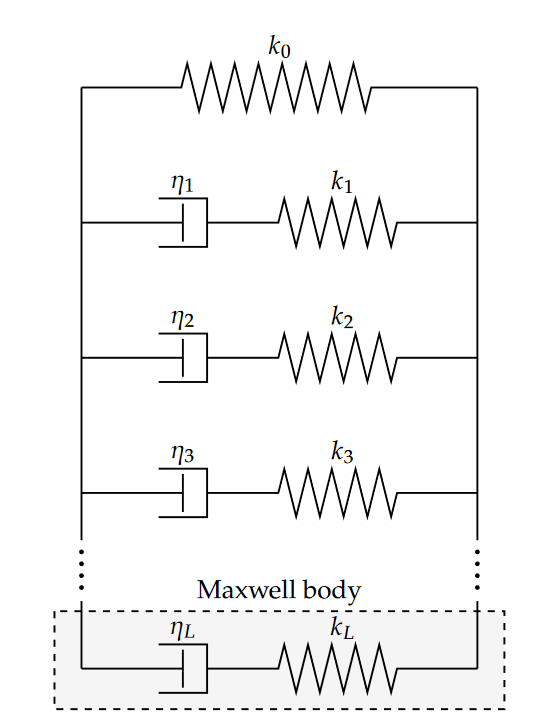
\includegraphics[width=7cm]{figures/gsls.png}
    \caption{Schematic diagram of a generalized standard linear solid (GSLS) composed of $L$ relaxation mechanisms (or Maxwell bodies), highlighted by the dashed square. $k_i$ ($i=1,\dots,L$) and $\eta_i$ ($i=1,\dots,L$) represent the elastic moduli and Newtonian viscosities, respectively, and are connected with the stress relaxation times $\tau^{\sigma l}$ and strain retardation times $\tau^{\varepsilon l}$ via $\tau^{\sigma l}=\frac{\eta_l}{k_l}$ and $\tau^{\varepsilon l}=\frac{\eta_l}{k_0}+\frac{\eta_l}{k_l}$ (after \cite{zener:48}; \cite{bohlen:02}).}
    \label{fig:gsls}
\end{figure}

With such a setup, new parameters are introduced:
\begin{itemize}
    \item $\tau^{\sigma l}$ and $\tau^{\varepsilon l}$: \textbf{stress-relaxation time} and \textbf{strain-retardation time}, respectively, of the $l$-th relaxation mechanism,
    \item $C^R$: \textbf{relaxed (or equilibrium) modulus}, i.e., $\lim_{t\to\infty} C(t)$ (where $C(t)$ represents the stress-impulse response function of the viscoelastic medium), corresponding to the low-frequency limit, i.e., $\omega = 0$.
\end{itemize}
According to \citet{Bai:16}, each relaxation process can be expressed in terms of the stress relaxation function $\Psi_{ijkl}(t)$ of the GSLS as\footnote{The differential calculus is firstly done in the Laplace domain and then back-transformed to the time domain.}
\begin{equation}
    \Psi_{ijkl}(t) = C_{ijkl}^R\,\left[1+\sum_{l=1}^{L} \left(\frac{\tau_{ij}^{\varepsilon l}}{\tau^{\sigma l}}-1\right) \exp\left(-\frac{t}{\tau^{\sigma l}}\right) \right] H(t)\;.
    \label{eq:psi}
\end{equation}
To simplify equation~\ref{eq:psi}, \citet{blanch:95} introduced the $\tau$-method, which demonstrates that the magnitude of attenuation in anisotropic media is directly quantified by the dimensionless matrix $\tau_{ij}$, which generally describes the \textbf{attenuation parameters} (directional variation of attenuation):
\begin{equation}
    \tau_{ij} = \frac{\tau_{ij}^{\varepsilon l}}{\tau^{\sigma l}}-1\;.
    \label{eq:taumethod}
\end{equation}
While $\tau_{ij}$ simply vanishes in the elastic case, as $\tau^{\sigma l} = \tau^{\varepsilon l}$, it should remain constant for all $L$ relaxation mechanisms in the viscoelastic case. In the previous studies, the attenuation was considered to be isotropic. We now included attenuation anisotropy as well.%This means that the number of independent parameters (i.e. $\tau^{\sigma l}$ and $\tau_{ij}$) for each element of $\Psi_{ijkl}$ reduces from 2$L$ to $L$+1 in the elastic case, while for the viscoelastic VTI case it is equal to $L$+4, i.e., $L$ for $\tau^{\sigma l}$ and 4 for $\tau_{ij}$. 

Considering the $\tau$-method, the explicit form of equation~\ref{eq:psi} is given by
\begin{equation}
    \Psi_{ijkl}(t) = C_{ijkl}^R\,\left[1+\sum_{l=1}^{L}\tau_{ij}\,\exp\left(-\frac{t}{\tau^{\sigma l}}\right) \right] H(t)\;.
    \label{eq:psi_2.0}
\end{equation}
Note that this relaxation function differs from the definition given in \citet{Bai:16}. In the special case of isotropy, $\Psi(t)$ reads  
\begin{subequations}
    \begin{align}
    \Psi_P(t) &= \pi\,\left[1+\sum_{l=1}^{L}\tau_P\,\exp\left(-\frac{t}{\tau^{\sigma l}}\right)\right]H(t)\;\\
    \Psi_S(t) &= \mu\,\left[1+\sum_{l=1}^{L}\tau_S\,\exp\left(-\frac{t}{\tau^{\sigma l}}\right)\right]H(t)\;.
    \end{align}
\end{subequations}

\citet{Bai:16} relate the relaxed modulus $C_{ijkl}^R$, corresponding to the model velocities, to the $C_{ijkl}$ modulus defined at the reference frequency $\omega_0 = 2\,\pi f_0$:
\begin{equation}
    C_{ijkl}^R = C_{ijkl}\bigg|_{\omega_0}\,\left(1+\sum_{l=1}^{L}\tau_{ij}\,\frac{(\omega_0\,\tau^{\sigma l})^2}{1+(\omega_0\,\tau^{\sigma l})^2} \right)^{-1}\;.
    \label{eq:relaxedmodulus_Bai}
\end{equation}
which, in the isotropic case, becomes
\begin{subequations}
\allowdisplaybreaks
\begin{align}
    \pi &= V_P^2\bigg|_{\omega_0}\;\rho\,\left(1+\sum_{l=1}^{L}\tau_P\,\frac{(\omega_0\,\tau^{\sigma l})^2}{1+(\omega_0\,\tau^{\sigma l})^2}\right)^{-1}\,,\\
    \mu &= V_S^2\bigg|_{\omega_0}\;\rho\,\left(1+\sum_{l=1}^{L}\tau_S\,\frac{(\omega_0\,\tau^{\sigma l})^2}{1+(\omega_0\,\tau^{\sigma l})^2}\right)^{-1}\;.
\end{align}
\end{subequations}

Following \citet{Zhu:06} and equation~\ref{eq:relaxedmodulus_Bai}, the mathematical matrix representation of $Q$ is given by 
\enlargethispage{\baselineskip}
\begin{equation}
    Q_{ij}^{-1}(\omega,\tau^{\sigma l},\tau_{ij}) = \frac{\sum_{l=1}^{L}\tau_{ij}\,\frac{\omega\tau^{\sigma l}}{1+(\omega\tau^{\sigma l})^2}}{1+\sum_{l=1}^{L}\tau_{ij}\,\frac{(\omega\tau^{\sigma l})^2}{1+(\omega\tau^{\sigma l})^2}}\;,
    \label{eq:Qinverse}
\end{equation}
with the substitutions $\tau = \tau_P$ and $\tau = \tau_S$, in the special case of isotropy, defining the level of attenuation for P- and S-waves, respectively. In general, the width of the frequency range in which a nearly constant $Q_{ij}$-spectrum can be simulated directly depends on the number of relaxation mechanisms (\cite{Bai:16}; \cite{Komatitisch:99}). When a GSLS consists of only one relaxation mechanism, i.e., $L=1$, a good estimate for $\tau$ is $\tau = \frac{2}{Q}$ (\cite{bohlen:02}).

At $t=0$, $\Psi_{ijkl}$ yields the \textbf{unrelaxed (or instantaneous) modulus} $C^U$, i.e., $\lim_{t\to0} C(t)$, which corresponds to the high-frequency limit, i.e., $\omega = \infty$.
\begin{equation}
    C_{ijkl}^U \equiv \Psi_{ijkl}\bigg|_{t=0} = C_{ijkl}^R\,(1+L\,\tau_{ij})\;,
\end{equation}
which, in the special case of isotropy, becomes
\begin{equation}
\allowdisplaybreaks
    \pi^U = \pi\,(1+L\,\tau_P)\quad\textrm{and}\quad\mu^U = \mu\,(1+L\,\tau_S)\;.
\end{equation}
By substituting $\Psi_{ijkl}(t)$ in the generalized stress-strain relation in viscoelastic media, and taking the time derivative on both sides, equation~\ref{eq:stress_strain_visco_2.0} becomes
\begin{equation}
\allowdisplaybreaks
    \begin{split}
    \dot{\sigma}_{ij} &= \dot{\Psi}_{ijkl}(t) \ast \dot{\varepsilon}_{kl} =\\ 
    &= C_{ijkl}^U\,\dot{\varepsilon}_{kl}-(C_{ijkl}^U-C_{ijkl}^R) \left[ \sum_{l=1}^{L}\frac{1}{\tau^{\sigma l}}\exp\left(-\frac{t}{\tau^{\sigma l}}\right) \right]H(t) \ast \dot{\varepsilon}_{kl}\;.
    \label{eq:stress_vti}
    \end{split}
\end{equation}
which, in isotropic anelastic media, is given by
\begin{equation}
    \sigma_{ij} = (\dot{\Psi}_P - 2\dot{\Psi}_S) \ast \theta\,\delta_{ij} + 2\,\dot{\Psi}_S \ast \varepsilon_{ij}\,.
    \label{eq:stress_iso_visco}
\end{equation}
In order to replace the convolution terms, \citet{Carcione:88} and \citet{robertsson:94} suggested that \textbf{memory variables} $r_{ij}^l$ corresponding to the $ij$-th component for the $l$-th relaxation mechanism should be introduced in such a way that
\begin{equation}
\allowdisplaybreaks
    r_{ij}^l = -\frac{2}{L\,\tau^{\sigma l}}\,(C_{ijkl}^U-C_{ijkl}^R)\exp\left(-\frac{t}{\tau^{\sigma l}}\right)H(t) \ast \dot{\varepsilon}_{kl}\;,
    \label{eq:r}
\end{equation}
which becomes by differentiating with respect to time and rearranging
% \begin{equation}
% \allowdisplaybreaks
%     \dot{r}_{ij}^l = \left[ -\frac{1}{\tau^{\sigma l}}(C_{ijkl}^U-C_{ijkl}^R)\,\exp\left(-\frac{t}{\tau^{\sigma l}}\right)\right] \left(-\frac{1}{\tau^{\sigma l}}\, H(t) + \delta(t)\right) \ast \dot{\varepsilon}_{kl}\;.
% \end{equation}
\begin{equation}
\allowdisplaybreaks
    \begin{split}
    \dot{r}_{ij}^l = &-\frac{2}{L\,\tau^{\sigma l}}\, \left[ -\frac{1}{\tau^{\sigma l}}(C_{ijkl}^U-C_{ijkl}^R)\,\exp\left(-\frac{t}{\tau^{\sigma l}}\right)H(t) \ast \dot{\varepsilon}_{kl} \right] - \\
    &- \frac{2}{L\,\tau^{\sigma l}}\,(C_{ijkl}^U-C_{ijkl}^R)\exp\left(-\frac{t}{\tau^{\sigma l}}\right)\,\delta(t) \ast \dot{\varepsilon}_{kl}\;.
    \end{split}
    \label{eq:r_dot}
\end{equation}
Introducing the expression of $r_{ij}^l$ at $t=0$ in equation~\ref{eq:r_dot}, I get
\begin{equation}
\allowdisplaybreaks
    \dot{r}_{ij}^l = - \frac{2}{L\,\tau^{\sigma l}}\,\left[ \frac{1}{2}\,(C_{ijkl}^U-C_{ijkl}^R)\left(\frac{\partial v_k}{\partial x_l}+\frac{\partial v_l}{\partial x_k}\right)+r_{ij}^l \right]\;.
    \label{eq:final_r_dot}
\end{equation}
Thus, equation \ref{eq:stress_vti} becomes
\begin{equation}
    \dot{\sigma}_{ij} = C_{ijkl}^U\,\left(\frac{\partial v_k}{\partial x_l}+\frac{\partial v_l}{\partial x_k}\right)+\sum_{l=1}^{L}r_{ij}^l\;.
    \label{eq:stress_vti_final}
\end{equation}
which, in the special case of isotropy, reads
\begin{equation}
    \dot \sigma_{ij} = \left[\pi\,(1+L\,\tau_{\varepsilon l}^P)-2\mu\,(1+L\,\tau_{\varepsilon l}^S)\right]\frac{\partial v_k}{\partial x_k}\,\delta_{ij} + \mu\,(1+L\,\tau_{\varepsilon l}^S)\left(\frac{\partial v_i}{\partial x_j}+\frac{\partial v_j}{\partial x_i}\right) + \sum_{l=1}^{L}r_{ij}^l\;.
\end{equation}

\subsection{Equations of motion for an anisotropic medium}
\label{ch:anisotropy}

\subsubsection{Seismic anisotropy and elasticity tensor}
As opposed to isotropy, which means homogeneity in all directions, anisotropy is the property of directional dependency. In seismics, anisotropy describes the directional or angle dependence of the velocity of seismic waves in a medium within the Earth, which can help to characterize preferred orientation and in-situ stress conditions. If the rock properties are aligned over a greater volume extending several wavelengths, they can create certain symmetries of seismic anisotropy (\cite{Thomsen:86}). Hexagonal (or cylindrical) symmetry is of particular interest in seismics, as it is relatively simple but can still approximate many actual situations in the Earth, for instance where sedimentary layers are neatly ordered. The most typical anisotropic medium that exhibits hexagonal symmetry is \textbf{transversely isotropic}, which means that the velocity normal to the bedding is slower than the one along it. Commonly investigated symmetries are \textbf{vertical-transverse isotropy} (VTI), with a vertical symmetry axis and infinite number of horizontal planes with isotropic behavior, and \textbf{tilted-transverse isotropy} (TTI), with a rotated symmetry axis, and thus properties changing with azimuth (\cite{Tsvankin:12}) (see Fig.~\ref{fig:tti}). \citet{Bai:16} developed a detailed numerical demonstration and analysis of vertical-transverse isotropic attenuation by 2D time-domain finite-difference modeling, while \citet{Oh:20} developed a similar tilted-transverse version. 
\begin{figure}[h!]
    \centering
    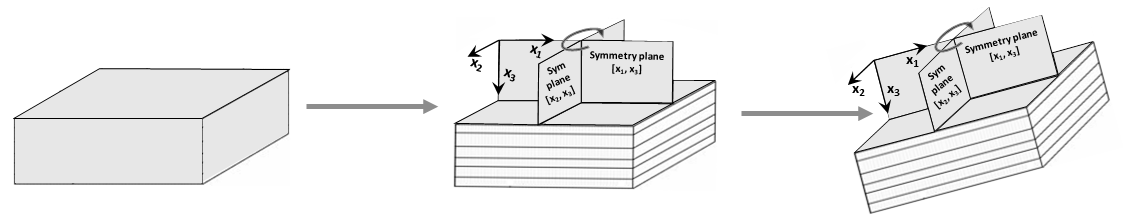
\includegraphics[width=0.9\textwidth]{figures/tti.png}
    \caption{From left to right: isotropic, VTI, and TTI media in a 3D Cartesian coordinate system with $(x_1,x_2,x_3) = (x,y,z)$ (modified after \cite{TGSwebsite}).}
    \label{fig:tti}
\end{figure}

The structure of the \textbf{stiffness tensor} $\mathbf{C_{ijkl}}$, previously introduced in subchapter~\ref{ch:eq_motion_elastic}, is the factor that determines the velocity and polarization of seismic waves for any propagation direction (\cite{Tsvankin:12}), thus uniquely describing the above-mentioned symmetries and their elastic moduli. In 3D, the fourth-order tensor had 36 independent components:
\begin{equation}
    \mathbf{C} = 
    \begin{pmatrix}
    c_{11} & c_{12} & c_{13} & c_{14} & c_{15} & c_{16} \\
    c_{12} & c_{22} & c_{23} & c_{24} & c_{25} & c_{26} \\
    c_{13} & c_{23} & c_{33} & c_{34} & c_{35} & c_{36} \\
    c_{14} & c_{24} & c_{34} & c_{34} & c_{45} & c_{46} \\
    c_{15} & c_{25} & c_{35} & c_{45} & c_{55} & c_{56} \\
    c_{16} & c_{26} & c_{36} & c_{46} & c_{56} & c_{66} 
    \end{pmatrix}\;,
    \label{eq:voigt_C}
\end{equation}
which is expressed in the Voigt notation (\cite{Voigt:10}).

For a polarization direction of the P-SV waves in 2D only, namely in the $x_1x_2$-plane, with the axes of the Cartesian coordinate system defined as $x_1$ for horizontal axis and $x_2$ for the vertical (depth) axis, the stiffness matrix becomes a $3 \times 3$ matrix with elements defining the $x_1x_1$-, $x_2x_2$-, and $x_1x_2$-directions. The stiffness tensor is then reduced to a combination of the Lam\'e parameters
\begin{equation}
    \mathbf{C} =
    \begin{pmatrix}
    c_{11} & c_{13} & c_{15} \\
    c_{13} & c_{33} & c_{35} \\
    c_{15} & c_{53} & c_{55} \\
    \end{pmatrix}\;.
    \label{eq:c_3x3}
\end{equation}
In the case of isotropic media, where the elastic behavior is independent of direction, only four elastic constants are independent and they simply reduce to
\begin{subequations}
\allowdisplaybreaks
    \begin{align}
        c_{11} &= c_{33}=\lambda+2\mu = \pi\;,\\
        c_{13} &= \lambda\;,\\
        c_{55} &= \mu\;,
    \end{align}
    \label{eq:c_iso_ij}
\end{subequations}
which form the elements of the stiffness matrix in 2D isotropic media:
\begin{equation}
    \mathbf{C}^\mathbf{iso} =
    \begin{pmatrix}
    \pi & \lambda & 0 \\
    \lambda & \pi & 0 \\
    0 & 0 & \mu \\
    \end{pmatrix}\;.
    \label{eq:c_iso_3x3}
\end{equation}
The P- and S-wave velocities will read then as
\begin{subequations}
\allowdisplaybreaks
    \begin{align}
        v_{P,ver} &= \sqrt{\frac{\lambda+2\mu}{\rho}}\;,\\
        v_{SV,ver} &= \sqrt{\frac{\mu}{\rho}}\;.
    \end{align}
\end{subequations}
In the case of 2D VTI media, Eq.~\ref{eq:c_3x3} reads (\cite{Thomsen:86})
\begin{equation}
    \mathbf{C}^\mathbf{VTI} =
    \begin{pmatrix}
    c_{11} & c_{13} & 0 \\
    c_{13} & c_{33} & 0 \\
    0 & 0 & c_{55} \\
    \end{pmatrix}\;.
    \label{eq:c_vti_3x3}
\end{equation}
Under the assumption of weak anisotropy, i.e., less than 20\%, these independent elastic constants have been combined by \citet{Thomsen:86} into the so-called \textbf{Thomsen anisotropic parameters} $\varepsilon$ and $\delta$ (dimensionless), such that they can better describe the seismic wave propagation:
\begin{subequations}
\allowdisplaybreaks
\begin{align}
    \varepsilon &= \frac{c_{11}-c_{33}}{2c_{33}}\;,\\
    \delta &= \frac{(c_{13}+c_{55})^2-(c_{33}-c_{55})^2}{2c_{33}\,(c_{33}-c_{55})}\;.
\end{align}
\end{subequations}
The vertical P- and S-wave velocities can also be expressed in terms of these elastic constants:
\begin{equation}
    v_{P,ver} \equiv \sqrt{\frac{c_{33}}{\rho}} \quad \textrm{and} \quad v_{SV,ver} \equiv \sqrt{\frac{c_{55}}{\rho}}\;.
    \label{eq:ver_vel}
\end{equation}

The angle-dependency of phase velocities, with the angle $\theta$ made by the symmetry axis of the VTI medium with the normal of the wavefront, is then given by the following approximate expressions:
\begin{subequations}
\allowdisplaybreaks
\begin{align}
    v_P(\theta) &\approx v_{P,ver}\,(1+\delta\,\sin^2\theta\cos^2\theta+\varepsilon\,\sin^4\theta)\;,\\
    v_{SV}(\theta) &\approx v_{SV,ver}\,\left(1+\frac{v_{P,ver}^2}{v_{SV,ver}^2}\,(\varepsilon-\delta)\sin^2\theta\,\cos^2\theta\right)\;,
    \label{eq:vel_angle}
\end{align}
\end{subequations}
with the maximal P-wave velocity given for a horizontal direction of wave propagation, while the maximal S-wave is reached at $45^{\circ}$:
\begin{subequations}
    \begin{align}
    v_{P,hor} &\equiv v_{P,ver}\,(1+\varepsilon)\;,\\
    v_{S,45^{\circ}} &\equiv \frac{v_{P,hor}^2\,(\varepsilon-\delta)}{4\,v_{SV,ver}}+v_{SV,ver}\;.
    \end{align}
    \label{eq:v_aniso}
\end{subequations}
In the case of $C_{ijkl}$ set along the symmetry axis, i.e., $\theta=0^{\circ}$, the elements of the stiffness matrix $\mathbf{C}^\mathbf{VTI}$ in Eq.~\ref{eq:c_vti_3x3} can be expressed as
\begin{equation}
    \renewcommand{\arraystretch}{2}
    \begin{pmatrix}
    c_{11} \\
    c_{33} \\
    c_{13} \\
    c_{55}
    \end{pmatrix} = 
    \begin{pmatrix}
    \rho\,v_{P,ver}^2\,(1+2\,\varepsilon) \\
    \rho\,v_{P,ver}^2 \\
    \rho\,\left(\sqrt{\left(v_{P,ver}^2-v_{SV,ver}^2\right)\left[v_{P,ver}^2\,\left(1+2\,\delta\right)-v_{SV,ver}^2\right]}-v_{SV,ver}^2\right) \\
    \rho\,v_{SV}^2 
    \end{pmatrix}\;.
    \label{eq:c_vti_thomsen}
\end{equation}
It can be observed that, while $\varepsilon$ quantifies the velocity difference for wave propagation along and perpendicular to the symmetry axis, $\delta$ controls the P-wave propagation for angles near the symmetry axis. 

In the case of TTI media, the stiffness matrix can be derived from the $\mathbf{C}^\mathbf{VTI}$ using the Bond transformation (\cite{Bond:43}; \cite{Carcione:07}) as suggested by \citet{Oh:20}: 
\begin{equation}
    \Tilde{\mathbf{C}}^\mathbf{TTI} = D(\theta_T)\,\mathbf{C}^{VTI}\,D^T(\theta_T)\;,
\end{equation}
with 
\begin{equation}
    D(\theta_T) = 
    \begin{pmatrix}
    \cos^{2}\theta_T & \sin^{2}\theta_T & 2\sin\theta_T\cos\theta_T \\
    \sin^{2}\theta_T & \cos^{2}\theta_T & -2\sin\theta_T\cos\theta_T \\
    -\sin\theta_T\cos\theta_T & \sin\theta_T\cos\theta_T & -\sin^{2}\theta_T \\
    \end{pmatrix}\,.
    \label{eq:d_vti}
\end{equation}
The matrix $\textit{D}$, rotated about the vertical axis in a counter-clockwise direction, represents a simple coordinate-rotation matrix, and the parameter $\theta_T$ denotes the tilt angle of the symmetry axis measured from the vertical. With its general expression given by
\begin{equation}
    \Tilde{\mathbf{C}}^\mathbf{TTI} = 
    \begin{pmatrix}
    \Tilde{c}_{11} & \Tilde{c}_{13} & \Tilde{c}_{15} \\
    \Tilde{c}_{13} & \Tilde{c}_{33} & \Tilde{c}_{35} \\
    \Tilde{c}_{15} & \Tilde{c}_{35} & \Tilde{c}_{55} \\
    \end{pmatrix}\,,
    \label{eq:c_tti_3x3}
\end{equation}
the $\tilde{c}_{ij}$ elements can be explicitly defined as
\begin{equation}
    \begin{pmatrix}
    \Tilde{c}_{11} \\
    \Tilde{c}_{33} \\
    \Tilde{c}_{13} \\
    \Tilde{c}_{55} \\
    \Tilde{c}_{15} \\
    \Tilde{c}_{35} \\
    \end{pmatrix} = 
    \begin{pmatrix}
    c_{11}\cos^{4}\theta_T+c_{33}\sin^{4}\theta_T+2\,(c_{13}+4\,c_{55})\,\sin^{2}\theta_T\cos^{2}\theta_T \\
    c_{11}\sin^{4}\theta_T+c_{33}\cos^{4}\theta_T+2\,(c_{13}+4\,c_{55})\,\sin^{2}\theta_T\cos^{2}\theta_T \\
    (c_{11}+c_{33}-4\,c_{55})\,\sin^{2}\theta_T\cos^{2}\theta_T+c_{13}\,(\sin^{4}\theta_T+\cos^{4}\theta_T) \\
    (c_{11}+c_{33}-2\,c_{13})\,\sin^{2}\theta_T\cos^{2}\theta_T+c_{55}\,(\cos^{2}\theta_T-\sin^{2}\theta_T)^2 \\
    (c_{13}-c_{11}+2\,c_{55})\,\cos^{3}\theta_T\sin\theta_T-(c_{13}-c_{33}+2\,c_{55})\,\cos\theta_T\sin^{3}\theta_T \\
    (c_{13}-c_{11}+2\,c_{55})\,\sin^{3}\theta_T\cos\theta_T-(c_{13}-c_{33}+2\,c_{55})\,\sin\theta_T\cos^{3}\theta_T \\ 
    \end{pmatrix}\;.
    \label{eq:c_tti_3x3_explicit}
\end{equation}

\subsubsection{Wave equations}
In this section, the velocity-stress formulation of the system of first-order differential equations that are the basis for the 2D FD anisotropic implementation is given. The wave equation for the 2D viscoelastic TTI media has been implemented recently into SOFI2D in order to verify the consistency of our extended wave equation formulation for anisotropic media with our previous formulation for isotropic media. 

For elastic media:
\begin{itemize}
    \item isotropic wave equations
        \begin{subequations}
        \allowdisplaybreaks
        \begin{align}
            % \rho\dot{v_x} &= \frac{\partial \sigma_{xx}}{\partial x} + \frac{\partial \sigma_{xz}}{\partial z}\;,\\
            % \rho\dot{v_z} &= \frac{\partial \sigma_{xz}}{\partial x} + \frac{\partial \sigma_{zz}}{\partial z}\;,\\
            \dot{\sigma}_{xx} &= \pi\,\frac{\partial v_x}{\partial x} + \lambda\,\frac{\partial v_z}{\partial z}\;,\\
            \dot{\sigma}_{zz} &= \lambda\,\frac{\partial v_x}{\partial x} + \pi\,\frac{\partial v_z}{\partial z}\;,\\
            \dot{\sigma}_{xz} &= \mu\,\left(\frac{\partial v_x}{\partial z} + \frac{\partial v_z}{\partial x}\right)\;.
            \label{eq:iso_elastic} 
        \end{align}
        \end{subequations}
    \item VTI wave equations
        \begin{subequations}
            \allowdisplaybreaks
            \begin{align}
            % \rho\dot{v_x} &= \frac{\partial \sigma_{xx}}{\partial x} + \frac{\partial \sigma_{xz}}{\partial z}\;,\\
            % \rho\dot{v_z} &= \frac{\partial \sigma_{xz}}{\partial x} + \frac{\partial \sigma_{zz}}{\partial z}\;,\\
            \dot{\sigma}_{xx} &= c_{11}\,\frac{\partial v_x}{\partial x} + c_{13}\,\frac{\partial v_z}{\partial z}\;,\\
            \dot{\sigma}_{zz} &= c_{13}\,\frac{\partial v_x}{\partial x} + c_{33}\,\frac{\partial v_z}{\partial z}\;,\\
            \dot{\sigma}_{xz} &= c_{55}\left(\frac{\partial v_x}{\partial z} + \frac{\partial v_z}{\partial x}\right)\;.
            \label{eq:vti_elastic} 
            \end{align}
        \end{subequations}
    \item TTI wave equations
        \begin{subequations}
            \allowdisplaybreaks
            \begin{align}
            % \rho\dot{v_x} &= \frac{\partial \sigma_{xx}}{\partial x} + \frac{\partial \sigma_{xz}}{\partial z}\;,\\
            % \rho\dot{v_z} &= \frac{\partial \sigma_{xz}}{\partial x} + \frac{\partial \sigma_{zz}}{\partial z}\;,\\
            \dot{\sigma}_{xx} &= \tilde{c}_{11}\,\frac{\partial v_x}{\partial x} + \tilde{c}_{13}\,\frac{\partial v_z}{\partial z}\ + \tilde{c}_{15}\,\left(\frac{\partial v_x}{\partial z} + \frac{\partial v_z}{\partial x}\right)\;,\\
            \dot{\sigma}_{zz} &= \tilde{c}_{13}\,\frac{\partial v_x}{\partial x} + \tilde{c}_{33}\,\frac{\partial v_z}{\partial z}\ + \tilde{c}_{35}\,\left(\frac{\partial v_x}{\partial z} + \frac{\partial v_z}{\partial x}\right)\;,\\
            \dot{\sigma}_{xz} &= \tilde{c}_{15}\,\frac{\partial v_x}{\partial x} + \tilde{c}_{35}\,\frac{\partial v_z}{\partial z}\ + \tilde{c}_{55}\,\left(\frac{\partial v_x}{\partial z} + \frac{\partial v_z}{\partial x}\right)\;.
            \label{eq:tti_elastic} 
            \end{align}
        \end{subequations}
\end{itemize}

The model parameters in the implementation of viscoelastic modeling are represented by the velocities and attenuation at $\omega_0$ and the relaxation frequencies $\tau^{\sigma l}$:
\begin{itemize}
    \item isotropic wave equations
        \begin{subequations}
        \allowdisplaybreaks
        \begin{align}
            \dot{\sigma}_{xx} &= \pi\,(1+L\,\tau^P)\,\left(\frac{\partial v_x}{\partial x} + \frac{\partial v_z}{\partial z} \right) - 2\,\mu\,(1+L\,\tau^S)\,\frac{\partial v_z}{\partial z} + \sum_{l=1}^{L}r_{xx}^l\;,\\   
            \dot{\sigma}_{zz} &= \pi\,(1+L\,\tau^P)\,\left(\frac{\partial v_x}{\partial x} + \frac{\partial v_z}{\partial z} \right) - 2\,\mu\,(1+L\,\tau^S)\,\frac{\partial v_x}{\partial x} + \sum_{l=1}^{L}r_{zz}^l\;,\\   
            \dot{\sigma}_{xz} &= \mu\,(1+L\,\tau^S)\,(\frac{\partial v_x}{\partial z}+\frac{\partial v_z}{\partial x})+\sum_{l=1}^{L}r_{xz}^l\;,\\    
            \dot{r}_{xx}^l &= -\frac{1}{\tau^{\sigma l}}\, \left[\pi\,\tau^P\,\left(\frac{\partial v_x}{\partial x} + \frac{\partial v_z}{\partial z} \right) - 2\,\mu\,\tau^S\,\frac{\partial v_z}{\partial z} + r_{xx}^l \right]\;,\\ 
            \dot{r}_{zz}^l &= -\frac{1}{\tau^{\sigma l}}\, \left[\pi\,\tau^P\,\left(\frac{\partial v_x}{\partial x} + \frac{\partial v_z}{\partial z} \right) - 2\,\mu\,\tau^S\,\frac{\partial v_x}{\partial x} + r_{zz}^l \right]\;,\\ 
            \dot{r}_{xz}^l &= -\frac{1}{\tau^{\sigma l}}\, \left[\mu\,\tau^S\,\left(\frac{\partial v_x}{\partial x} + \frac{\partial v_z}{\partial z} \right) + r_{xz}^l \right]\;.
        \end{align}
        \end{subequations}
    \item VTI media
        \begin{subequations}
        \allowdisplaybreaks
        \begin{align}
            \dot{\sigma}_{xx} &= c_{11}^U\,\frac{\partial v_x}{\partial x}+c_{13}^U\,\frac{\partial v_z}{\partial z}+\sum_{l=1}^{L}r_{xx}^l\;,\\   
            \dot{\sigma}_{zz} &= c_{13}^U\,\frac{\partial v_x}{\partial x}+c_{33}^U\,\frac{\partial v_z}{\partial z}+\sum_{l=1}^{L}r_{zz}^l\;,\\   
            \dot{\sigma}_{xz} &= c_{55}^U\,\left(\frac{\partial v_x}{\partial z}+\frac{\partial v_z}{\partial x}\right)+\sum_{l=1}^{L}r_{xz}^l\;,\\     
            \dot{r}_{xx}^l &= -\frac{1}{\tau^{\sigma l}}\,\left(c_{11}^R\,\tau_{11}\,\frac{\partial v_x}{\partial x}+c_{13}^R\,\tau_{13}\,\frac{\partial v_z}{\partial z}+r_{xx}^l\right)\;,\\
            \dot{r}_{zz}^l &= -\frac{1}{\tau^{\sigma l}}\, \left(c_{13}^R\,\tau_{13}\,\frac{\partial v_x}{\partial x}+c_{33}^R\,\tau_{33}\,\frac{\partial v_z}{\partial z}+r_{zz}^l \right)\,,\\
            \dot{r}_{xz}^l &= -\frac{1}{\tau^{\sigma l}}\, \left[c_{55}^R\,\tau_{55}\,\left(\frac{\partial v_x}{\partial z}+\frac{\partial v_z}{\partial x}\right)+r_{xz}^l \right]\;.
            \label{eq:wave_eq_vti}
        \end{align}
        \end{subequations}
    \item TTI media
        \begin{subequations}
        \allowdisplaybreaks
        \begin{align}
            \dot{\sigma}_{xx} &= \Tilde{c}_{11}^U\,\frac{\partial v_x}{\partial x}+\Tilde{c}_{13}^U\,\frac{\partial v_z}{\partial z}+\Tilde{c}_{15}\,\left(\frac{\partial v_x}{\partial z}+\frac{\partial v_z}{\partial x}\right)+\sum_{l=1}^{L}r_{xx}^l\;,\\   
            \dot{\sigma}_{zz} &= 
            \Tilde{c}_{13}^U\,\frac{\partial v_x}{\partial x}+\Tilde{c}_{33}^U\,\frac{\partial v_z}{\partial z}+\Tilde{c}_{35}\,\left(\frac{\partial v_x}{\partial z}+\frac{\partial v_z}{\partial x}\right)+\sum_{l=1}^{L}r_{zz}^l\;,\\
            \dot{\sigma}_{xz} &= \Tilde{c}_{15}^U\,\frac{\partial v_x}{\partial x}+\Tilde{c}_{35}^U\,\frac{\partial v_z}{\partial z}+\Tilde{c}_{55}\,\left(\frac{\partial v_x}{\partial z}+\frac{\partial v_z}{\partial x}\right)+\sum_{l=1}^{L}r_{xz}^l\;,\\
            -\tau_{\sigma l}\,\dot{r}_{xx}^l &=  \Tilde{c}_{11}^R\,\tau_{11}\,\frac{\partial v_x}{\partial x}+\Tilde{c}_{13}^R\,\tau_{13}\,\frac{\partial v_z}{\partial z}+\Tilde{c}_{15}^R\,\tau_{13}\,\left(\frac{\partial v_x}{\partial z}+\frac{\partial v_z}{\partial x}\right)+r_{xx}^l\;,\\
            -\tau_{\sigma l}\,\dot{r}_{zz}^l &=  \Tilde{c}_{33}^R\,\tau_{33}\,\frac{\partial v_z}{\partial z}+\Tilde{c}_{13}^R\,\tau_{13}\,\frac{\partial v_x}{\partial x}+\Tilde{c}_{35}^R\,\tau_{35}\,\left(\frac{\partial v_x}{\partial z}+\frac{\partial v_z}{\partial x}\right)+r_{zz}^l\;,\\
            -\tau_{\sigma l}\,\dot{r}_{xz}^l &=  \Tilde{c}_{55}^R\,\tau_{55}\,\left(\frac{\partial v_z}{\partial x}+\frac{\partial v_x}{\partial z}\right)+\Tilde{c}_{15}^R\,\tau_{15}\,\frac{\partial v_x}{\partial x}+\Tilde{c}_{35}^R\,\tau_{35}\,\frac{\partial v_z}{\partial z}+r_{xz}^l\;.
            \label{eq:wave_eq_tti}
        \end{align}
        \end{subequations}
\end{itemize}

\subsubsection{Numerical results}
In order to emphasize the pronounced effects of anisotropy on the wavefield, we show the directional variation of P- and S-waves in a highly anisotropic VTI medium (Fig.~\ref{fig:snapshots}). The P-wave velocity increases significantly towards the horizontal direction ($\theta = \ang{90}$). The angular variation of S-wave depends upon polarity. Horizontally polarized S-waves (SH) are fastest in the horizontal direction, whereas vertically polarized S-waves (SV) have a maximum velocity around $\theta = \ang{45}$.

We also compare numerical results for the elastic and viscoelastic
case to highlight the effects of attenuation. Whereas attenuation mainly leads to a frequency dependent decay of amplitudes with distance, anisotropy affects both travel times and amplitudes considerably. Note for instance the strong deformation of both the P- and SV-wave wavefronts in the VTI case according to the directional variation of phase velocities depicted in Fig.~\ref{fig:snapshots}. Furthermore, in the VTI medium the SV-wave develops significant amplitude anomalies along the diagonal direction ($\theta = \ang{45}$), known as cusps. The counter-clockwise rotation of the symmetry axis in the TTI case by $\theta = \ang{30}$ is clearly visible and has a strong impact on the radiation pattern of the wavefield for both P- and SV-waves.

\begin{figure}[h!]
    \centering
    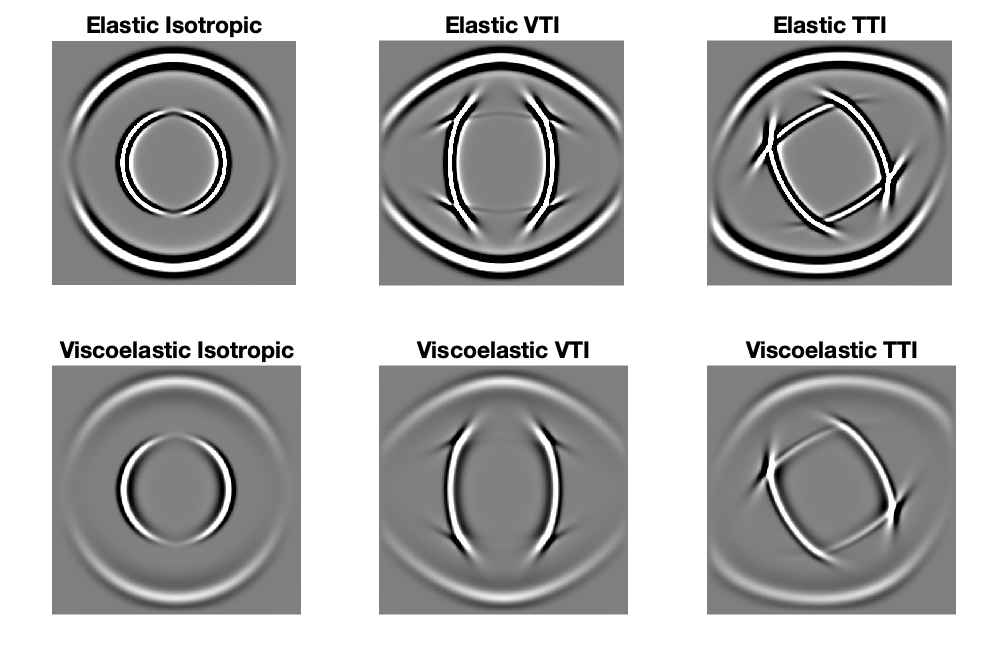
\includegraphics[width=0.9\textwidth]{figures/modeling}
    \caption{Snapshots of vertical component of particle velocity excited by a vertical point force. The snapshots show P- and SV-waves and the effects of attenuation and VTI and TTI anisotropy. The homogeneous anisotropic VTI model is that of Greenhorn shale. In the TTI model, the symmetry axis has been rotated counter-clockwise $\theta = \ang{30}$. Attenuation is assumed to be isotropic and described by $\sigma_P=\sigma_S=\SI{0.25}{}$, $L=1$.}
    \label{fig:snapshots}
\end{figure}

\subsection{Solution of the wave equation by finite differences}
\label{elastic_FD_Code}
Solving the above-mentioned wave equations analytically is only possible for very simple models. In more realistic cases, wave propagation can only be estimated using numerical approaches. One of them is the \textbf{finite-differences (FD) method}, in which spatial and temporal derivatives in the wave equations are approximated by FD operators, making it numerical efficient and relatively straightforward to implement. This approximation requires the discretization of the wave equation in both space and time using a Cartesian coordinate system of equidistant grid spacing. Thus, the continuous space coordinates $x$ and $z$ and the time vector $t$ are replaced by their discrete form in a way that $x = i\,\Delta h$, $z = j\,\Delta h$, and $t = n\,\Delta t$, with $i,j$ representing the position of a specific grid point and $n$ referring to a specific \textbf{time step}; $\Delta h$ denotes the spatial distance between two adjacent grid points (i.e., \textbf{grid spacing}) and $\Delta t$ the difference between two successive time steps (i.e., time sampling interval). Therefore, every grid point is located in the interval  $i \in N | [1,NX]$, $j \in N | [1,NY]$ and $n \in N | [1,NT]$, where $NX$, $NY$ and $NT$ are the number of discrete spatial grid points and time steps, respectively. 

Two types of operators can be distinguished, forward and backward operators $D^+,D^-$. The derivative of a function $y$ with respect to a variable $x$ can be approximated by the following operators:  
\begin{subequations}
    \begin{align}
        {D^+_x} y &= \frac{y{[i+1]} - {y[i]}}{\Delta h}\;,\\
        {D^-_x} y &= \frac{y{[i]}-y{[i-1]}}{\Delta h}\;.
    \end{align}
    \label{eq:3}
\end{subequations}

\subsubsection{Standard staggered grid}
\label{ssg}
The propagation of elastic waves in the stress-velocity formulation can be modeled on a standard staggered grid (SSG), which ensures stability and high accuracy (\cite{virieux:86}; \cite{levander:88}). On such a grid, different components of one physical parameter are defined at different staggered points. Fig.~\ref{fig:ssg} shows the locations of viscoelastic wavefield parameters and material parameters on the SSG. Fig.~\ref{fig:ssg} shows the locations of wavefield parameters: the two different components of the particle velocity $v_i$ are distributed over two different staggered locations, at half grid points; the stress components $\sigma_{ij}$ are distributed over two different locations: the diagonal stresses on full grid points, and the shear stresses on half grid points; the same holds for the memory variables.

The material parameters, namely $\rho$, $\mu$, $\tau$, and the $c_{ij}$ components need to be locally averaged, i.e., calculated from neighboring grid points. The averaging of material parameters is critical for the accuracy at strong discontinuities \cite{zahradnik:93,falk:98,moczo:02}. To obtain stable results, arithmetic averaging  must be used for the density $\rho$ and attenuation parameter $\tau^S$, and harmonic averaging is required for the shear modulus (\cite{fellinger:95,graves:96,falk:98,vossen:02,moczo:02}):
\begin{subequations}
\allowdisplaybreaks
    \begin{align}
        \rho_x[j,i+\frac{1}{2}] &= \frac{\rho[j,i]+\rho[j,i+1]}{2}\;,\\
        \rho_y[j+\frac{1}{2},i] &= \frac{\rho[j,i]+\rho[j+1,i]}{2}\;,\\
        \tau^S_{xy}[j+\frac{1}{2},i+\frac{1}{2}] &= \frac{\tau^S[j,i]+\tau^S[j,i+1]+\tau^S[j+1,i+1]+\tau^S[j+1,i]}{4}\;,\\
        \mu_{xy}[j+\frac{1}{2},i+\frac{1}{2}] &= \frac{4}{\mu^{-1}[j,i]+\mu^{-1}[j,i+1]+\mu^{-1}[j+1,i+1]+\mu^{-1}[j+1,i]}\;.
        \label{eq:stress_vti2}
    \end{align}
\end{subequations}
This averaging procedure satisfies the condition of traction continuity across the interface between two media on standard staggered grids (\cite{moczo:02}). Harmonic averaging of the shear modulus $\mu$ yields higher accuracy than arithmetic averaging for modeling Scholte waves propagating along fluid-solid interfaces (\cite{falk:98}). What is more, our numerical tests show that arithmetic averaging of the shear modulus across free surfaces leads to instabilities; harmonic averaging produces stable simulations. 
\begin{figure}[ht!]
    \centering
    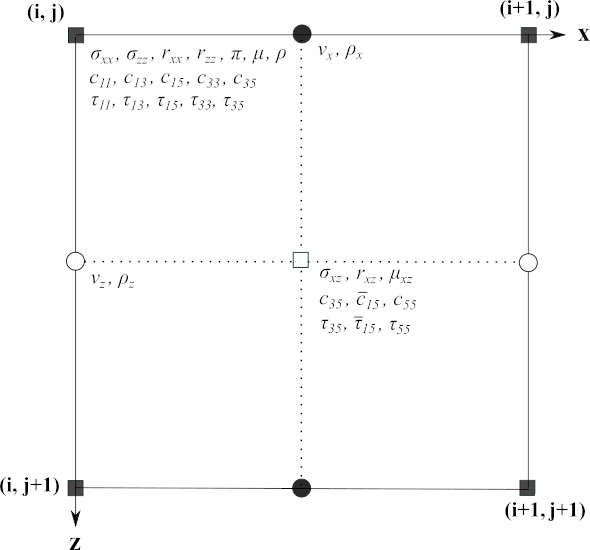
\includegraphics[width=10cm]{figures/ssg_final.png}
    \caption{Distribution of viscoelastic anisotropic wavefield- and material parameters on an elementary finite-difference cell in the standard staggered grid (modified after \cite{virieux:86}).
    At half grid point, i.e., $(i+\frac{1}{2},j+\frac{1}{2})$, $\bar{c}_{15}$ and $\bar{\tau}_{15}$ are harmonically- and arithmetically-averaged, respectively.}
    \label{fig:ssg}
\end{figure}

\subsubsection{Free surface and interfaces on a SSG}
% For the SSG the location of the free surface is defined by the plane going through the staggered position of the particle velocity $v_y$ and shear stress $\sigma_{xy}$ (Fig.~...). As a consequence the computation of the curl (S-wave component) and divergence (P-wave component) of the particle velocity wavefield is not accurate at the free surface because $v_x$ is located outside and $v_y$ inside the medium.
The determination of the actual location of an interface between two media on the SSG is not a trivial task. Only in the case that interfaces are aligned with the grid the interface location can be determined. On curved interfaces, however, the interface location cannot be determined exactly due to the staggered grid representation of the model. 

Varying topography in FD modeling can only be represented by staircases (Fig.~\ref{fig:ssg}). As the true topography can show strong variations in height, the topography on the SSG needs to be carefully handled. Following the distribution of physical parameters in an SSG cell, with the vertical component of the particle velocity calculated at half grid points, all vertical point sources and receivers must be located at half grid points, too, so that any numerical issues are avoided during modeling (Fig.~\ref{fig:ssg_topo}). 
\begin{figure}[ht!]
    \centering
    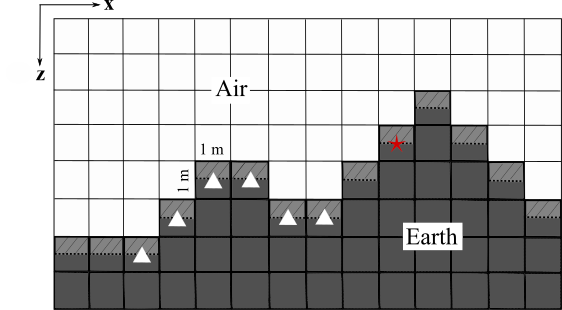
\includegraphics[width=9cm]{figures/topo.png}
    \caption{Topography on the standard staggered grid. Red star: source point; white triangles: receivers. Note the staircases that appear due to quantization of the elevation values.}
    \label{fig:ssg_topo}
\end{figure}

The interface between the elastic medium and air at the surface is very important when trying to model surface waves or multiple reflections in a marine environment. Since all stresses in the normal direction at this interface vanish in a way that $\sigma_{xy} = \sigma_{yy}=0.0$; this boundary condition is called (stress) {\textbf{free surface}}. Two types of implementations are common. \textcolor{red}{In the implicit definition of the free surface, a small layer with the acoustic parameters of air
($v_P=\SI{300}{m/s}$, $v_S=\SI{0}{m/s}$, $\rho=\SI{1.25}{kg/m^3}$) is placed on top of the model}. One advantage of the implicit definition of the free surface is the easy implementation of topography on the FD grid, however to get accurate results for surface waves or multiples, this approach requires a fine spatial sampling of the FD grid near the free surface. An explicit free surface can be implemented by using the mirroring technique by Levander, which leads to stable and accurate solutions for plain interfaces (\cite{levander:88}, \cite{robertsson:95}). If the planar free surface is located at grid point $j=h$, the stress at this point is set to zero and the stresses below the free surface are mirrored with an inverse sign:
\begin{equation}
\begin{split}
        \sigma_{yy}[h,i] &= 0\,,\\
        \sigma_{yy}[h-1,i] &= - \sigma_{yy}[h+1,i]\,,\\
        \sigma_{xy}[h-\frac{1}{2},i+\frac{1}{2}] &= - \sigma_{xy}[h+\frac{1}{2},i+\frac{1}{2}]\,,\\
        \sigma_{xy}[h-\frac{3}{2},i+\frac{1}{2}] &= - \sigma_{xy}[h+\frac{3}{2},i+\frac{1}{2}]\,.
\end{split}
\end{equation}

When updating the stress component $\sigma_{xx}=\Delta t\, \pi (v_{xx} + v_{yy}) -2 {\Delta t}\, \mu\, v_{yy}$ at the free surface only horizontal particle velocities should be used because vertical derivatives over the free surface lead to instabilities (\cite{levander:88}). 
The vertical derivative of $v_{yy}$ can be replaced by using the boundary condition at the free surface:
\begin{equation}
\begin{split}
    \sigma_{yy} &= {\Delta t}\, \pi\left(v_{xx} + v_{yy}\right)  - 2 {\Delta t}\, \mu\, v_{xx} = 0\;,\\
    v_{yy} &= - \frac{\pi-2\mu}{\pi} v_{xx}\;.
\end{split}
\end{equation}
Therefore equation ... can be written as
\begin{equation}
\sigma_{xx}={\Delta t}\left(4\mu -\frac{(2\mu)^2}{\pi} \right) v_{xx}\;.
\end{equation}

\subsubsection{Discretization of the wave equation}
\label{discretization}
The discretization of the linear stress-strain relationship at time step \textit{n} leads to the following system of equations:
\begin{equation}
\allowdisplaybreaks
    \begin{split}
        v_{xx}\,[j,i] & \approx \frac{v_x [j,i+\frac{1}{2}]-v_x[j,i-\frac{1}{2}]}{dh}\;,\\
        v_{yy}\,[j,i] & \approx \frac{v_y [j+\frac{1}{2},i]-v_y[j-\frac{1}{2},i]}{dh}\;,\\
        v_{yx}\,[j+\frac{1}{2},i+\frac{1}{2}] & \approx \frac{v_y [j+\frac{1}{2},i+1]-v_y [j+\frac{1}{2},i]}{\Delta h}\;,\\
        v_{xy}\,[j+\frac{1}{2},i+\frac{1}{2}] & \approx \frac{v_x  [j+1,i+\frac{1}{2}]-v_x [j,i+\frac{1}{2}]}{\Delta h}\;,\\
        \sigma_{xy}^{n}\,[j+\frac{1}{2},i+\frac{1}{2}] &= \sigma_{xy}^{n-1}\,[j+\frac{1}{2},i+\frac{1}{2}] + \Delta t \cdot \mu_{xy} \,[j+\frac{1}{2},i+\frac{1}{2}] \cdot\\
        & \cdot \biggl(v_{xy}\,[j+\frac{1}{2},i+\frac{1}{2}] + v_{yx} \,[j+\frac{1}{2},i+\frac{1}{2}]\biggr)\;,\\
        \sigma_{xx}^{n}\,[j,i] &= \sigma_{xx}^{n-1}\,[j,i] + \Delta t \cdot \pi [j,i] \cdot \biggl(v_{xx} [j,i] - v_{yy}\,[j,i] \biggr) - \\
        & -2 \cdot \Delta t \cdot \mu [j,i] \cdot v_{xx} [j,i]\;,\\
        \sigma_{yy}^{n}\,[j,i] &= \sigma_{yy}^{n-1}\,[j,i] + \Delta t \cdot \pi\,[j,i] \cdot \biggl(v_{xx}\,[j,i] - v_{yy}\,[j,i] \biggr) -\\
        & -2 \cdot dt \cdot \mu [j,i] \cdot v_{yy}\,[j,i]\;.
        \label{eq:discr_stress}
    \end{split}
\end{equation}
 
The discretization of the momentum equation leads to the following system of equations:
\begin{equation}
\allowdisplaybreaks
    \begin{split}
        vtt_x\,[j,i+\frac{1}{2}] &= \biggl(\sigma_{xx} [j,i+1] - \sigma_{xx}[j,i] + \sigma_{xy}[j+\frac{1}{2},i] - \sigma_{xy}[j-\frac{1}{2},i] \biggr)\;,\\
        vtt_y\,[j+\frac{1}{2},i] &= \biggl(\sigma_{xy}[j,i+\frac{1}{2}] - \sigma_{xy}[j,i-\frac{1}{2}] + \sigma_{yy} [j+1,i] - \sigma_{yy} [j,i] \biggr)\;,\\
        v_x^{n}\,[j,i+\frac{1}{2}] &= v_x^{n-1} [j,i+\frac{1}{2}] + \frac{\Delta t}{\Delta h}\cdot\rho_x  [j,i+\frac{1}{2}] \cdot vtt_x\,[j,i+\frac{1}{2}]\;,\\
        v_y^{n}\,[j+\frac{1}{2},i] &= v_y^{n-1} [j+\frac{1}{2},i] + \frac{\Delta t}{\Delta h} \cdot \rho_y [j+\frac{1}{2},i] \cdot vtt_y\,[j+\frac{1}{2},i]\;.\\
        \label{eq:discr_momentum}
    \end{split}
\end{equation}

\subsubsection{Accuracy of FD operators}
\label{accuracy}
The derivation of the FD operators in the last section was a simple replacement of the partial derivatives by finite differences. In the following more systematic approach, the first derivative of a variable $f$ at a grid point $i$ is estimated by a Taylor series expansion (\cite{jastram:92a}):
\begin{equation}
    \begin{split}
        (2k-1)\frac{\partial f}{\partial x}\biggr|_i &= \frac{1}{\Delta h}(f_{i+(k-1/2)}-f_{i-(k-1/2)}) + \\
        & +\frac{1}{\Delta h}\sum_{l=2}^N \frac{((k-\frac{1}{2}) (\Delta h)^{2l-1}}{(2l-1)!}\frac{\partial^{(2l-1)}f}{\partial
        x^{(2l-1)}}\biggr|_i+{\mathcal{O}}(\Delta h)^{2N}\;.
    \end{split}
\end{equation}

For an operator with length $2N$, $N$ equations are added with a weight $\beta_k$:
\begin{equation}
    \begin{split}
        \biggl[\sum_{k=1}^{N} \beta_k (2k-1)\biggr]\frac{\partial f}{\partial x}\biggr|_i &= \frac{1}{\Delta h} \sum_{k=1}^{N} \beta_k (f_{i+(k-1/2)}-f_{i-(k-1/2)}) +\\
        &+\frac{1}{\Delta h}\sum_{k=1}^{N} \sum_{l=2}^N \beta_k \frac{((k-\frac{1}{2})(\Delta h)^{2l-1}}{(2l-1)!}\frac{\partial^{(2l-1)}f}{\partial
        x^{(2l-1)}}\biggr|_i+{\mathcal{O}}(\Delta h)^{2N}\;.
    \end{split}
\end{equation}

The case $N=1$ leads to the FD operator derived in the last section, which has a length of $2N=2$. The Taylor series is truncated after the first term (${\mathcal{O}}(\Delta h)^{2}$). Therefore, this operator is called {\textbf{2nd order FD operator}} which refers to the truncation error of the Taylor series and not to the order of the approximated derivative. To understand equation %\ER{op_acc:2} ...
better, we estimate a {\textbf{4th order FD operator}}. This operator has the length $2N=4$ or $N=2$. The sums in Eq. %\ER{op_acc:2} 
lead to:
\begin{equation}
    \begin{split}
        (\beta_1+3 \beta_2) \frac{\partial f}{\partial x}\biggr|_i &= \frac{1}{\Delta h}(\beta_1(f_{i+1/2}-f_{i-1/2})+\beta_2(f_{i+3/2}-f_{i-3/2})) +\\
        & +\frac{\Delta h^3}{\Delta h}\biggl[\beta_1\frac{1}{8 \cdot 3!}+\beta_2\frac{27}{8 \cdot 3!}\biggr]\frac{\partial^3 f}{\partial x^3}\biggr|_i\;.
    \end{split}
\end{equation}

The weights $\beta_k$ can be calculated by the following approach: 
The factor in front of the partial derivative on the LHS of Eq. %\ER{op_acc:3} 
should equal 1, therefore $\beta_1+3\beta_2=1$. The coefficients in front of $\frac{\partial^3 f}{\partial x^3}\biggr|_i$ on the RHS of Eq. %\ER{op_acc:3} 
should vanish: $\beta_1+27\beta_2=0$. The weights $\beta_k$ can be estimated by solving the matrix equation:
\begin{equation}
    \left(
    \begin{array}{ll}
    1 & 3 \\
    1 & 27 \\
    \end{array}
    \right)\cdot \hspace{0.2 cm}
    \left(
    \begin{array}{l}
    \beta_1 \\
    \beta_2 \\
    \end{array}
    \right)
    =
    \left(
    \begin{array}{l}
    1 \\
    0 \\
    \end{array}
    \right) \notag
\end{equation}

The resulting coefficients are $\beta_1=9/8$ and $\beta_2=-1/24$. Therefore, the 4th order backward- and forward operators are:
\begin{equation}
\begin{split}
    \frac{\partial f}{\partial x}\biggr|_{i+1/2} &= \frac{1}{\Delta h}[\beta_1 (f_{i+1}-f_i)+\beta_2 (f_{i+2}-f_{i-1})] \hspace{1 cm} \text{forward operator}\;,\\
    \frac{\partial f}{\partial x}\biggr|_{i-1/2} &= \frac{1}{\Delta h}[\beta_1 (f_{i}-f_{i-1})+\beta_2 (f_{i+1}-f_{i-2})] \hspace{1 cm} \text{backward operator}\;.
\end{split}
\end{equation}

The coefficients $\beta_i$ in the FD operator are called {\textbf{Taylor coefficients}}. The accuracy of higher order FD operators can be improved by seeking for FD coefficients $\beta_k$ that approximate the first derivative in a certain frequency range (\cite{holberg:87}). 
These numerically optimized coefficients are called {\textbf{Holberg coefficients}}.

\subsubsection{Adams-Bashforth fourth-order accurate time integrators}
\label{adams-bashforth}
To improve the precision of the temporal discretization the Adams-Bashforth fourth-order accurate time integrator can be used. 
The staggered Adams-Bashforth method (ABS) is a multi-step method that uses previously calculated wavefields to increase the accuracy order in time. In \citet{bohlen2015higher2} and \citet{bohlen2015higher} a detailed study of the performance of the ABS method in 1D and 3D is given. The analysis shows that the numerical dispersion is much lower than that of the widely used second-order leapfrog method. However numerical dissipation is introduced by the ABS method. In simulation experiments the convincing improvements of accuracy of the fourth-order ABS method is verified. For instance, in a realistic elastic 3D scenario the computing time reduces by a factor of approximately 2.2, whereas the memory requirements increase by approximately the same factor. The ABS method thus provides an alternative strategy to increase the time accuracy by investing computer memory instead of computing time.

In the following we provide an extract of \citet{bohlen2015higher2} to demonstrate the underlying theory. Additionally, seismograms of different temporal orders of accuracy and an analysis of the numerical simulation error are shown.

In SOFI2D, only a fourth-order accurate Adams-Bashforth time integrator is implemented, due to the superior performance over third-order.

\paragraph{Theory}
For the sake of simplicity, we illustrate the staggered ABS method using the 1D acoustic wave equation in velocity-stress formulation
\begin{subequations}
    \begin{align}
        \frac{\partial p(x,t)}{\partial t} &= - \pi (x)\,\frac{\partial v(x,t)}{\partial x}  \notag\;,\\
        \frac{\partial v(x,t)}{\partial t} &= -\rho^{-1}(x)\,\frac{\partial p(x,t)}{\partial x}\;.
        \label{waveequation}
    \end{align}
\end{subequations}
The wavefield variables are the pressure $p(x,t)$ and the particle velocity $v(x,t)$. The material is described by the P-wave modulus $\pi (x)$ and the mass density $\rho(x)$. For simplicity we omit the temporal ($t$) and spatial dependencies ($x$)  in the following.

Using the conventional second order staggered grid approximation to the first order time derivative we obtain
\begin{subequations}
    \begin{align}
    \frac{p |^{n+1/2}-p|^{n-1/2}}{\Delta t} &= - \pi\,\frac{\partial v}{\partial x}\bigg |^n  + \mathcal{O}(\Delta t^2)\;,\\ 
    \frac{v|^n-v|^{n-1}}{\Delta t} &= -\rho^{-1}\,\frac{\partial p}{\partial x}\bigg |^{(n-1/2)} + \mathcal{O}(\Delta t^2)\;.
    \label{2ndorder}
    \end{align}
\end{subequations}

This results in the conventional explicit second order accurate time-stepping (leapfrog) scheme
\begin{subequations}
    \begin{align}
        p|^{n+1/2} &= p|^{n-1/2} - \Delta t\,\pi\,\frac{\partial v}{\partial x}\bigg |^n  + \mathcal{O}(\Delta t^2)\;,\\
        v|^n &= v|^{n-1} -\Delta t\,\rho^{-1}\,\frac{\partial p}{\partial x}\bigg |^{(n-1/2)}  + \mathcal{O}(\Delta t^2)\;,
        \label{2ndorderexplicit}
    \end{align}
\end{subequations}
which requires no additional storage of the wavefield variables $p$ and $v$. 

With the ABS-method the order of the temporal integration  can be increased by using previous time levels of the right hand sides of Eq.~\ref{2ndorder} (\cite{ghrist2000staggered}). The ABS-method thus requires the storage of previous time levels of spatial derivatives of the pressure $p$ and particle velocity $v$. The time update for the ABS-method thus reads
\begin{subequations}
    \begin{align}
        p|^{n+1/2} &= p|^{n-1/2} - \Delta t\,\pi \sum_{k=0}^{M-1} a_k\,\frac{\partial v}{\partial x}\bigg |^{n-k}   + \mathcal{O}(\Delta t^M)\;,\\
        v|^n &= v|^{n-1} -\Delta t\,\rho^{-1}  \sum_{k=0}^{M-1} a_k\,\frac{\partial p}{\partial x}\bigg |^{(n-1/2-k)}  + \mathcal{O}(\Delta t^M)\;.
        \label{absmethod}
    \end{align}
\end{subequations}
The weights for the time accuracy orders $M=2,3,4$ are given in Table~\ref{absweights}. 
\begin{table}[ht]
    \centering
    \caption{\label{absweights}Weights used for the summation of previous time levels in the Adams-Bashforth method (\protect\cite{ghrist2000staggered}).}
    \begin{tabular}{c|c|c|c|c}
    $M$ & $a_0$ & $a_1$ & $a_2$ & $a_3$  \\ \hline
    2 & 1             &  0           &  0           &     0   \\
    3 &  25/24     &  -1/12         & 1/24   & 0   \\
    4 & 13/12      &  -5/24      &  1/6       &  -1/24     \\
    \end{tabular}
\end{table}

\paragraph{Accuracy in 1-D}
We first compare seismograms calculated with the 1D ABS-method using Eq.~\ref{absmethod} for different orders of accuracy in time ($M$). We use a 1D homogeneous acoustic  medium with a wave velocity of $c=\SI{3000}{m/s}$ and constant density of $\rho=\SI{2000}{kg/m^3}$. The source signal is a Ricker signal with a center frequency of \SI{60}{Hz}. We choose a large source-receiver distance of 120 dominant wavelength to emphasize the effects of numerical dispersion and numerical dissipation in the synthetic seismograms. The spatial derivatives are computed with high accuracy using a centered staggered FD stencil of 8th order accuracy.  The spatial grid spacing is held constant at $\Delta x=0.4$\,m corresponding to approximately 14 grid points per dominant wavelength. Discrepancies to the analytical solution (time-shifted Ricker signal) are thus mainly caused by the chosen time step interval $\Delta t$ and the order of the temporal discretization ($M=2,3,4$). The numerical results for Courant numbers $r=c \Delta t/\Delta x=0.4, 0.2, 0.1$ and temporal orders of accuracy $M=2, 3, 4$ are compared with the analytical solution in Fig.~\ref{fig_1dfdseis}. For a large Courant number of $r=0.4$ (corresponding to a large time step interval) and second order approximation of the time derivative ($M=2$) we can observe a large time dispersion error causing a leading phase with high amplitude (Fig.~\ref{fig_1dfdseis}, top-left). Fig.~\ref{fig_1dfdseis} compares two ways to reduce this time discretization error. The conventional way is to  stay with the given temporal accuracy order (typically $M=2$) and then reduce the time step interval, i.e., Courant number. The resulting waveforms are shown in the rows of Fig.~\ref{fig_1dfdseis}.

Reducing the Courant number (time step interval) will increase the computation time proportional to $1/r$.  The alternative  way proposed in this study is to increase the order of the temporal discretization with the ABS-method which requires to store $M-1$ previously calculated spatial derivatives of wavefields. The resulting waveforms are shown in the columns of Fig.~\ref{fig_1dfdseis}.

In Fig.~\ref{fig_1dfdseis} we see that the simulation accuracy increases with decreasing Courant number and increasing accuracy order. In order to quantify the corresponding numerical simulation error we calculated the normalized L2-misfit between the numerical and analytical solution for different Courant numbers and accuracy orders $M=2,3,4$. 

In Fig.~\ref{fig_L2} we plot the normalized L2-misfit over the number of time steps $NT=T/\Delta t=T c/(r \Delta x)$ where the propagation time of waves is held fixed at $T=0.24$\,s. We can observe the expected higher order reduction of the simulation accuracy which reduces proportional to $\Delta t^{M}$ or $NT^{-M}$. For a given accuracy level of $E=0.1\%$ (horizontal line in Fig.~\ref{fig_L2}) the required numbers of time steps are 39233, 13938, and 8704 for $M=2,M=3$ and $M=4$, respectively. The number of time steps thus reduces  to $36\%$  and $22\%$  when we increase the temporal order from $M=2$ to $M=3$ and $M=4$, respectively (Fig.~\ref{fig_L2}). The ABS methods thus allows to significantly decrease the number of time steps and thus to save computing time. 
\begin{figure}[h!]
\centering
    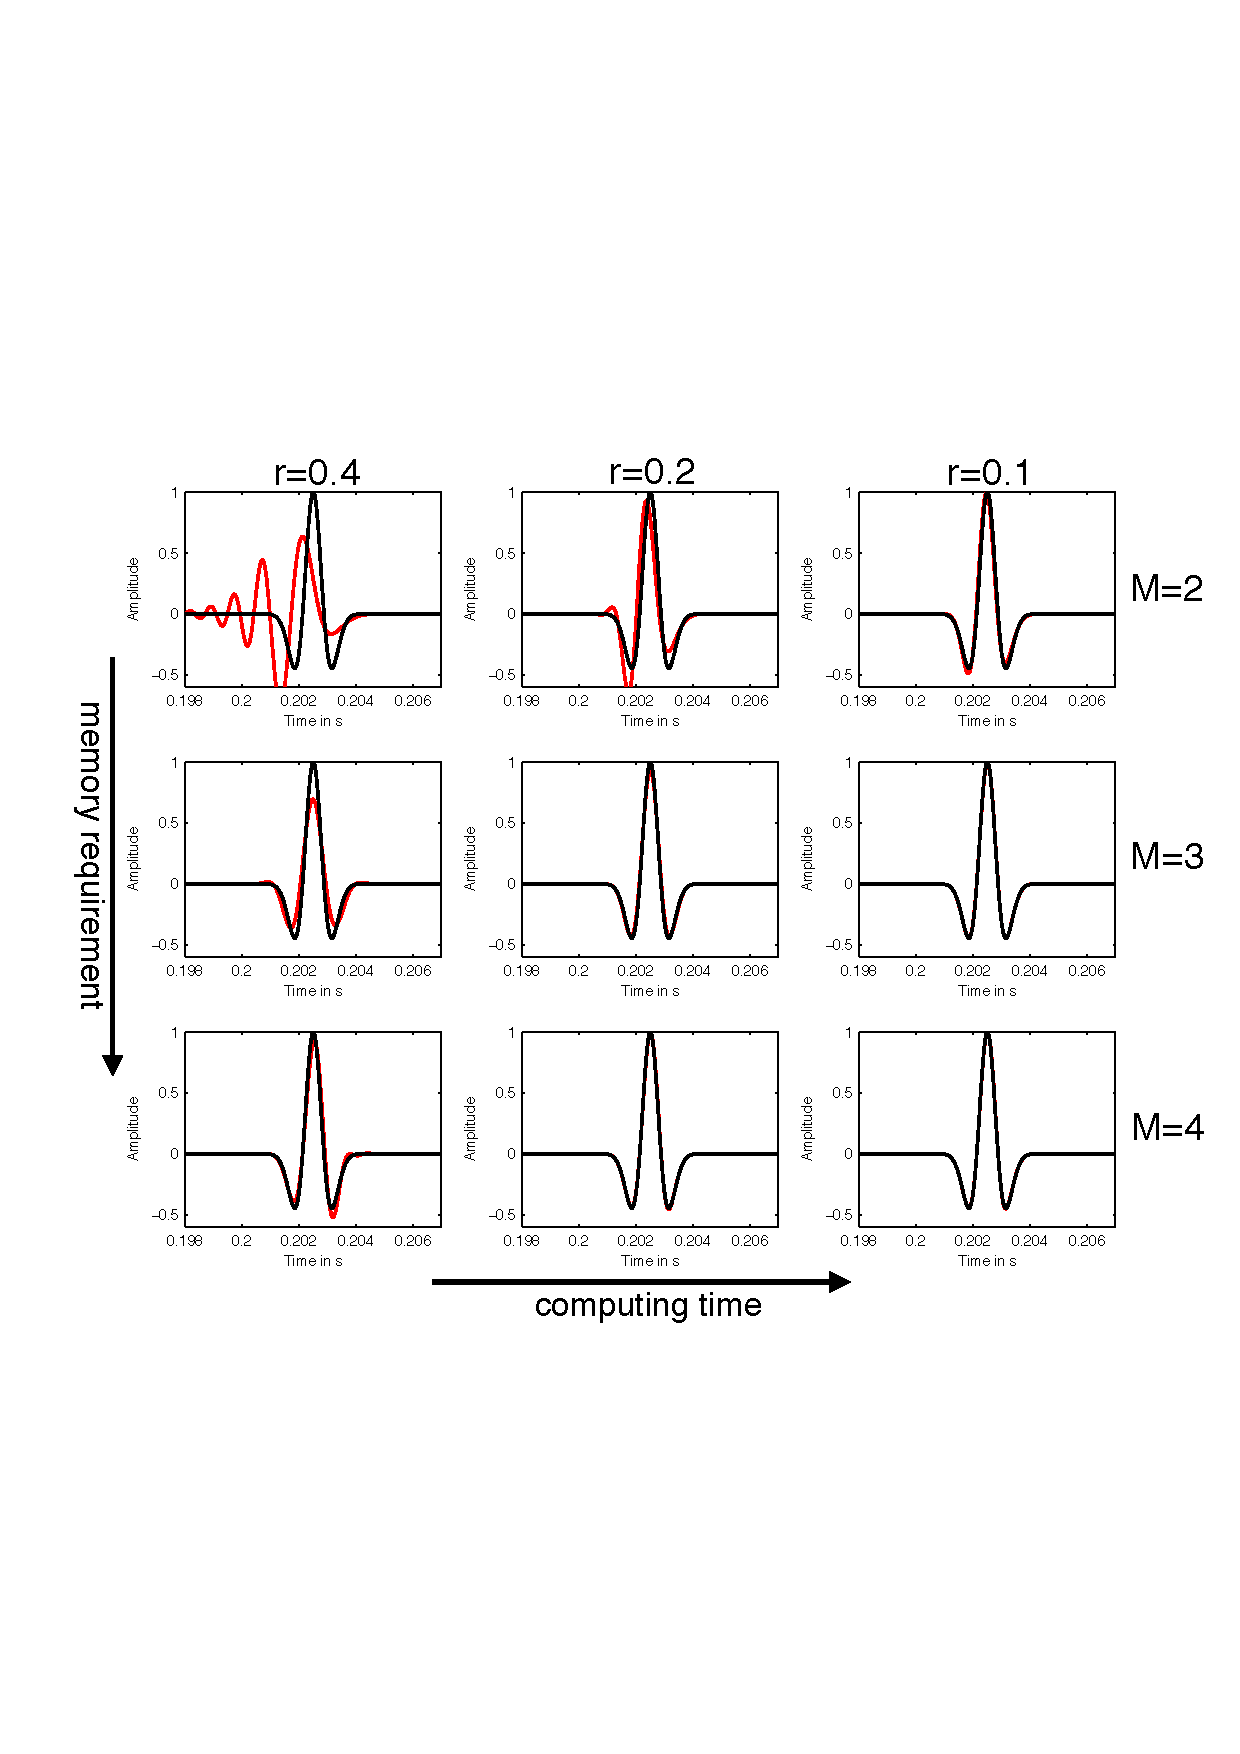
\includegraphics[width=\textwidth]{figures/seismo.pdf}
    \caption{Seismograms (red lines) calculated for the 1-D case for different Courant numbers $r$ and accuracy orders $M$. $M=2$ corresponds to the classical second order leapfrog scheme (Eq.~\ref{2ndorder}). $M=3,4$ correspond to the multi-step ABS method (Eq.~\ref{absmethod}). The analytical solution is plotted as a black line.}
    \label{fig_1dfdseis}
\end{figure}

\begin{figure}[h]
\centering
    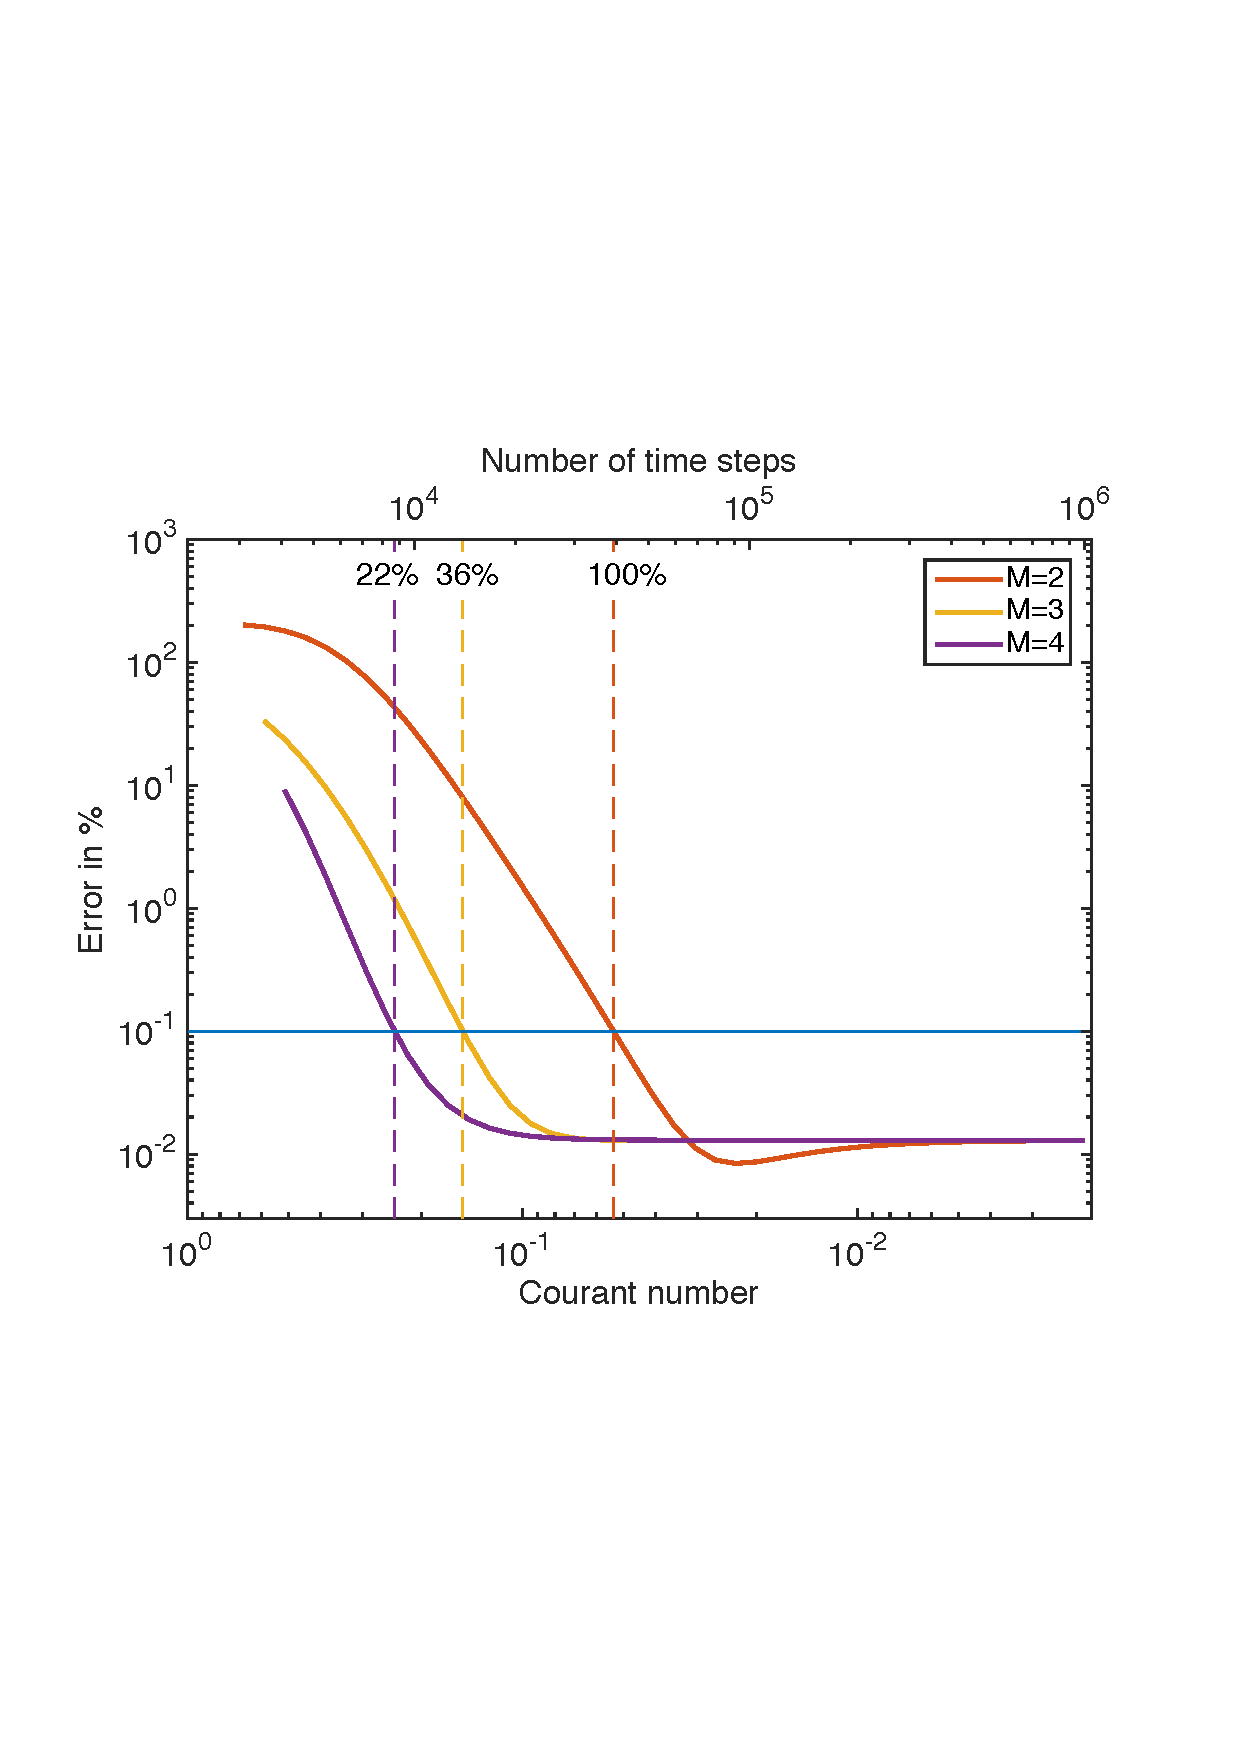
\includegraphics[scale=0.7]{figures/error_1D_courant}
    \caption{Relative error of 1D simulations (Fig.~\ref{fig_1dfdseis}). The normalized L2 norm is plotted over the required number of time steps ($NT$). The temporal accuracy orders are $M=2,3,4$. The spatial accuracy is fixed at order $N=8$. The number of time steps to achieve a given accuracy of $E=0.01\%$ (horizontal line) reduce to $36\%$ and $22\%$ for the temporal orders $M=3$ and $M=4$, respectively. For large $NT$ (small time step intervals) the error converges to the fixed error of the spatial discretization.}
    \label{fig_L2}
\end{figure}

\subsubsection{Absorbing Boundary Conditions}
Due to limited computational resources, the FD grid has to be as small as possible. To model problems with an infinite extension in different directions, e.g., a full or half-space problem,  an artificial absorbing boundary condition has to be applied. A very effective way to damp the waves near the boundaries are {\textbf{Perfectly Matched Layers (PMLs)}}. This can be achieved by a coordinate stretch of the wave equations in the frequency domain \cite{komatitsch:07}. The coordinate stretch creates exponentially decaying plane wave solutions in the absorbing boundary frame. The PMLs are only reflectionless if the exact wave equation is solved. As soon as the problem is discretized (for example using finite differences) you are solving an approximate wave equation and the analytical perfection of the PML is no longer valid. In SOFI2D, a damping profile $d_x$ after \citet{collino2001application} is implemented:
\begin{equation}
    d_x(x) = d_0\left(\frac{x}{L}\right)^n\;,
\end{equation}
where $L$ denotes the width of the absorbing frame and $d_0$ is a function of the theoretical reflection coefficient $R$:
\begin{equation}
    d_0 = -\left(n+1\right) V_{PML}\frac{log(R)}{2L}\;,
\end{equation}
where $V_{PML}$ denotes the typical P-wave velocity of the medium in the absorbing boundary frame. A reflection coefficient of $R=1 \times 10^{-4}$ is assumed. The PMLs are damping the seismic waves by a factor 5-10 more effective than the conventional absorbing boundary frame.

\subsection{Numerical artifacts and instabilities}
\label{num_instab}
To avoid numerical artifacts and instabilities during a FD modeling run, a spatial and temporal sampling condition for the wavefield has to be satisfied. These will be discussed in the following two sections. 

\subsubsection{Grid Dispersion}
\label{grid-dispersion}
The first question when building a FD model is: What is the maximum spatial grid point distance $\Delta h$, for a correct sampling of the wavefield? To answer this question we take a look at this simple example: The particle displacement in $x$-direction is defined by a sine function:
\begin{equation}
   v_x=\sin\biggl(2 \pi \frac{x}{\lambda}\biggr) \;,
   \label{eq:gri_disp}
\end{equation}
where $\lambda$ denotes the wavelength. When calculating the derivation of this function analytically at $x=0$ and setting $\lambda=\SI{1}{m}$ we get:
\begin{equation}
    \frac{d v_x}{d x}\biggl|_{x=0} = \frac{2 \pi}{\lambda} \cos\biggl(2 \pi \frac{x}{\lambda}\biggr)\biggl|_{x=0}=2 \pi\;.
    \label{eq:gri_disp_anal}
\end{equation}
In the next step the derivation is approximated numerically by a staggered 2nd order finite-difference operator:
\begin{equation}
    \frac{d v_x}{d x}\biggl|_{x=0} \approx \frac{v_x(x+\frac{1}{2}\Delta x)-v_x(x-\frac{1}{2}\Delta x)}{\Delta x}\biggl|_{x=0}=\frac{\sin \biggl(\frac{2 \pi (\frac{1}{2}{\Delta x})}{\lambda} \biggr)-\sin \biggl(\frac{2 \pi (\frac{1}{2}{dx})}{\lambda} \biggr)}{\Delta x}\;.
    \label{eq:gri_disp_num}
\end{equation}

Using the Nyquist-Shannon sampling theorem it should be sufficient to sample the wavefield with $\Delta x = \lambda/2$. In Table~\ref{grid_disp.1} the numerical solutions (Eq.~\ref{eq:gri_disp_num}) and the analytical solution (Eq.~\ref{eq:gri_disp_anal}) are compared for different sample intervals $\Delta x = \lambda /n$, where $n$ is the number of gridpoints per wavelength. For the case $n=2$, which corresponds to the Nyquist-Shannon theorem, the numerical solution is $\frac{d v_x}{d x}|_{x=0}=4.0$, which is not equal with the analytical solution $2 \pi$. A refinement of the spatial sampling of the wavefield results in an improvement of the finite difference solution. For $n=16$ the numerical solution is accurate to the second decimal place. The effect of a sparsely sampled pressure field is illustrated in Fig.~\ref{fig_homo_grid} for a homogeneous block model with stress free surfaces. The dimensions of the FD grid are fixed and the central frequency of the source signal is increased systematically.  When using a spatial sampling of 16 grid points per minimum wavelength (\ref{fig_homo_grid}, top) the wavefronts are sharply defined. For $n=4$  grid points a slight numerical dispersion of the wave occurs (\ref{fig_homo_grid}, center). This effect is obvious when using the Nyquist criterion ($n=2$) (\ref{fig_homo_grid}, bottom). Since the numerical calculated wavefield seem to be dispersive this numerical artefact is called {\textbf{grid dispersion}}. 

To avoid the occurence of grid dispersion the following criteria for the spatial grid spacing $\Delta h$ has to be satisfied:
\begin{equation}
    \Delta h \le \frac{\lambda_{min}}{n} = \frac{V_{min}}{{n}\,f_{max}}\;,
    \label{eq:dh}
\end{equation}
where $\lambda_{min}$ denotes the minimum wavelength, $V_{min}$ the minimum velocity in the model, and $f_{max}$ is the maximum frequency of the source signal.  

Depending on the accuracy of the used FD operator the parameter $n$ is different. In Table~\ref{grid_disp.2} n is listed for different FD operator lengths and types (Taylor and Holberg operators). The Holberg coefficients are calculated for a minimum dispersion error of $0.1\%$ at $3 f_{max}$. For short operators n should be chosen relatively large, so the spatial grid spacing is small, while for longer FD operators n is smaller and the grid spacing can be larger. 
\begin{figure}[ht!]
\centering
    \begin{subfigure}[b]{0.45\textwidth}
        \centering
        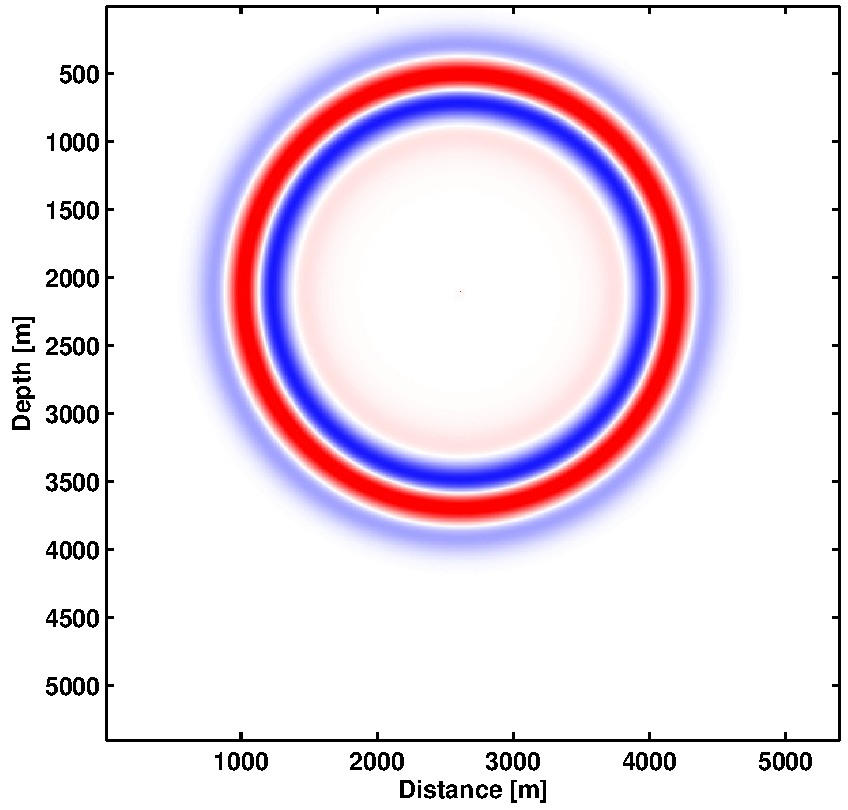
\includegraphics[width=\textwidth]{figures/homogenous_grid_n_16_5.pdf}
        \caption{}
    \end{subfigure}
    \hfill
    \begin{subfigure}[b]{0.45\textwidth}
        \centering
        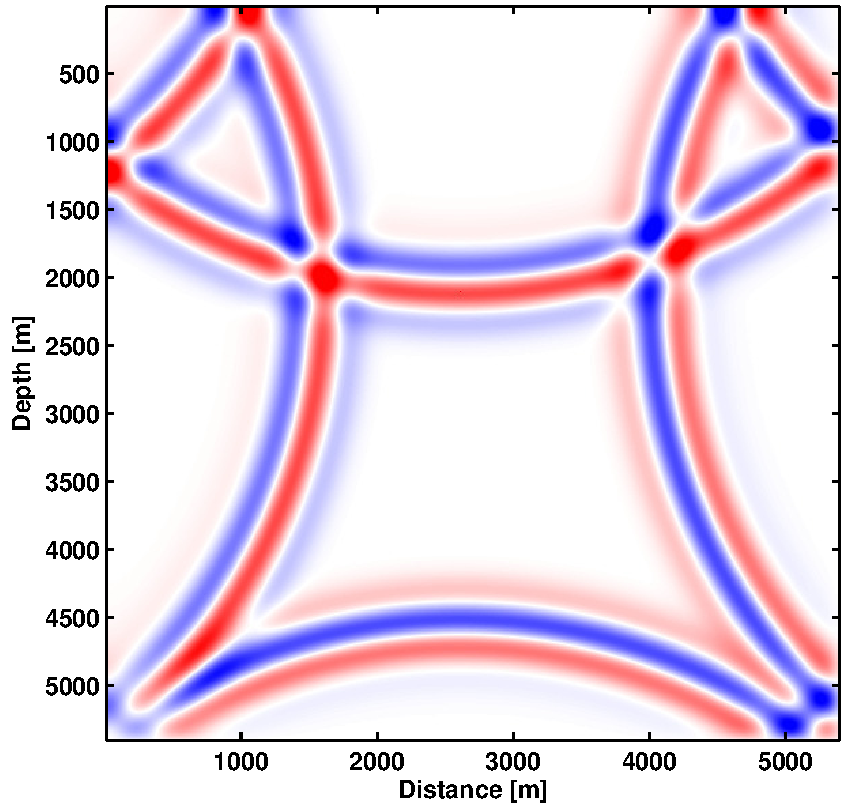
\includegraphics[width=\textwidth]{figures/homogenous_grid_n_16_10.pdf}
        \caption{}
    \end{subfigure}
    \vfill
    \begin{subfigure}[b]{0.45\textwidth}
        \centering
        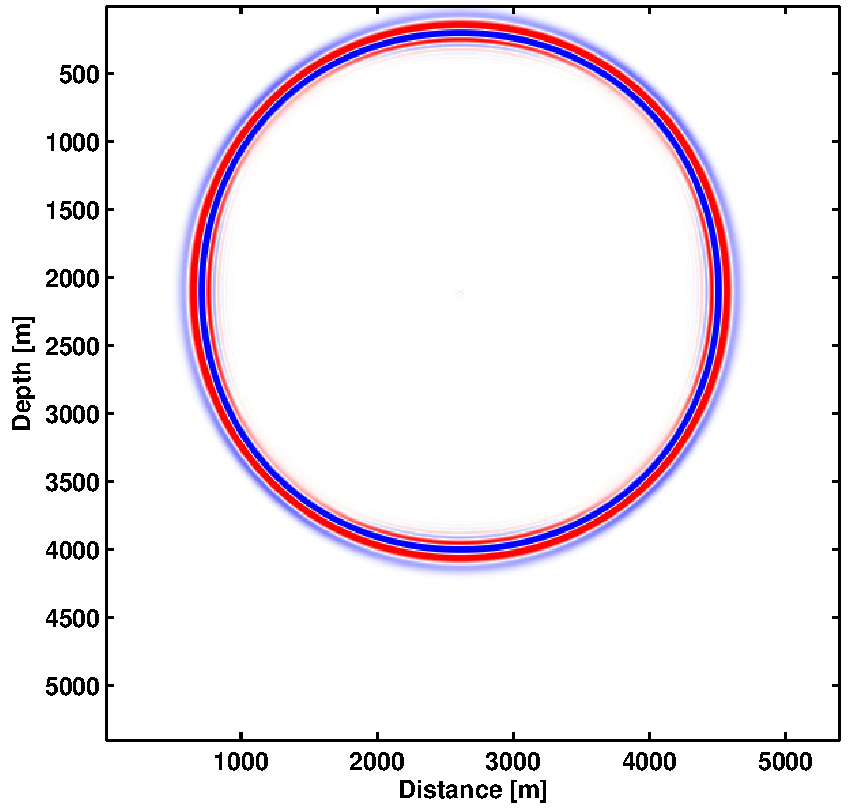
\includegraphics[width=\textwidth]{figures/homogenous_grid_n_4_5.pdf}
        \caption{}
    \end{subfigure}
    \hfill
    \begin{subfigure}[b]{0.45\textwidth}
        \centering
        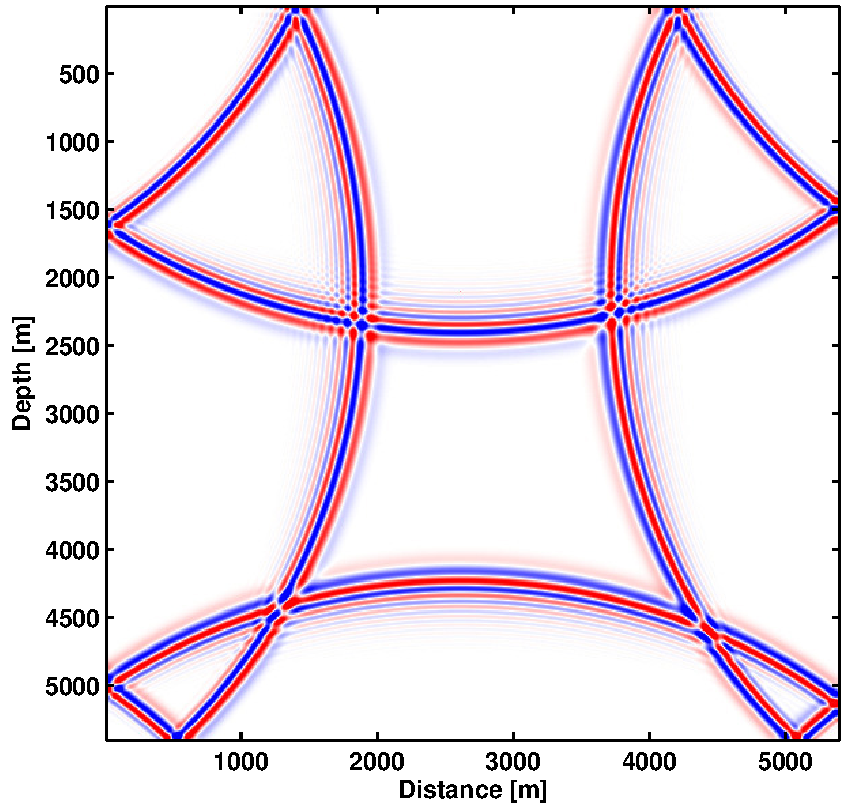
\includegraphics[width=\textwidth]{figures/homogenous_grid_n_4_10.pdf}
        \caption{}
    \end{subfigure}
    \vfill
    \begin{subfigure}[b]{0.45\textwidth}
        \centering
        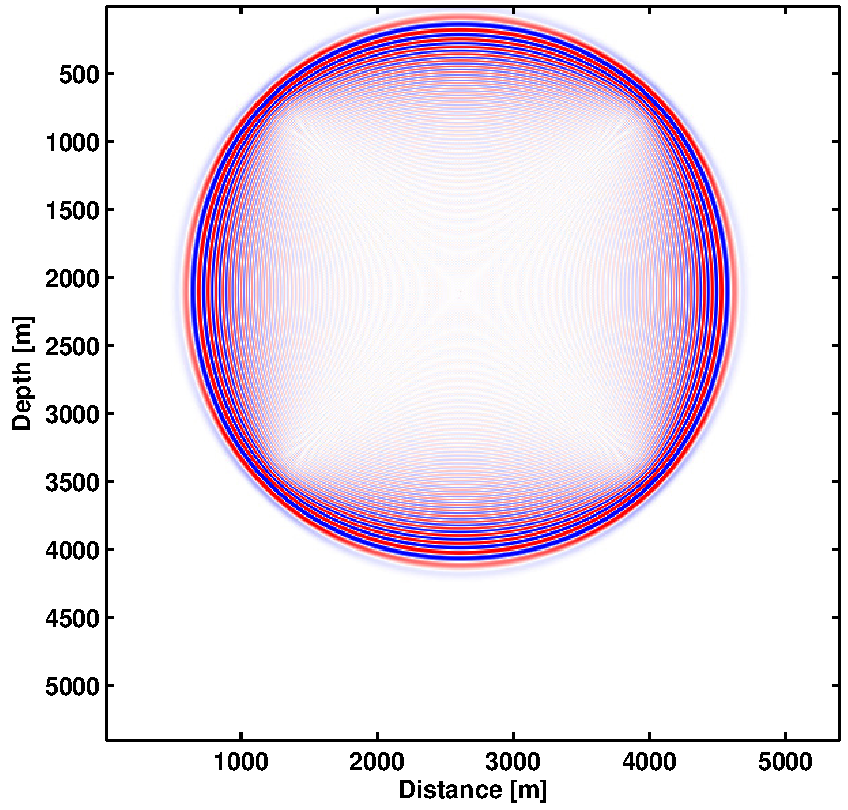
\includegraphics[width=\textwidth]{figures/homogenous_grid_n_2_5.pdf}
        \caption{}
    \end{subfigure}
    \hfill
    \begin{subfigure}[b]{0.45\textwidth}
        \centering
        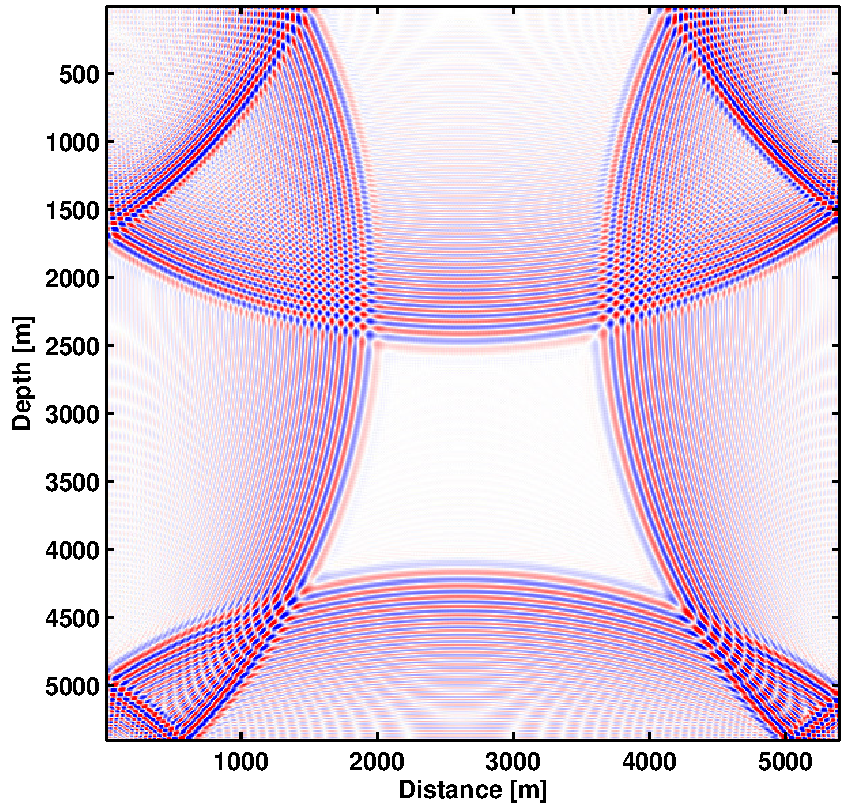
\includegraphics[width=\textwidth]{figures/homogenous_grid_n_2_10.pdf}
        \caption{}
    \end{subfigure}
\caption{\label{grid_disp_pics} The influence of grid dispersion in FD modeling: Spatial sampling of the wavefield using $n=16$ (top), $n=4$ (center) and $n=2$ gridpoints (bottom) per minimum wavelength.}
\label{fig_homo_grid}
\end{figure}

\begin{table}[hbt]
\caption{\label{grid_disp.1} Comparison of the analytical solution Eq.~\ref{eq:gri_disp_anal} with the numerical solution Eq.~\ref{eq:gri_disp_num} for different grid spacing $\Delta x = \lambda /n$.}
\centering
\begin{tabular}{c|c|c}
    \textbf{n} &  \textbf{$\mathbf{\Delta x}\,$ [m]} & \textbf{$\mathbf{\frac{d v_x}{d x}|_{x=0}}$} \\ \hline 
    analytical & - & $2\pi \approx 6.283$ \\ 
    2 & $\lambda/2$ & 4.0 \\ 
    4 & $\lambda/4$ & 5.657 \\ 
    8 & $\lambda/8$ & 6.123 \\ 
    16 & $\lambda/16$ & 6.2429 \\ 
    32 & $\lambda/32$ & 6.2731
\end{tabular}
\end{table}
 
\begin{table}[hbt]
\caption{\label{grid_disp.2} The number of grid points per minimum wavelength $n$ for different orders (2nd-12th) and types (Taylor and Holberg) of FD operators. For the Holberg coefficients n is calculated for a minimum dispersion error of $0.1\%$ at $3\,f_{max}$.}
\centering
\begin{tabular}{c|c|c}
    \textbf{FDORDER} & \textbf{n (Taylor)} & \textbf{n (Holberg)} \\ \hline 
    2nd   &   12       &  12         \\
    4th   &   8        &  8.32       \\
    6th   &   6        &  4.77       \\
    8th   &   5        &  3.69       \\ 
    10th  &   5        &  3.19       \\
    12th  &   4        &  2.91       
\end{tabular}
\end{table} 

\subsubsection{The Courant Instability}
\label{courant}
Beside the spatial, the temporal discretization has to satisfy a sampling criterion to ensure the stability of the FD code. If a 
wave is propagating on a discrete grid, then the timestep $\Delta t$ has to be less than the time for the wave to travel between two adjacent grid 
points with grid spacing $\Delta h$. For an elastic 2D grid this means mathematically:
\begin{equation}
    \Delta t \le \frac{\Delta h}{h \sqrt{2} V_{max}}\;,
    \label{courant_crit}
\end{equation}
where $V_{max}$ is the maximum velocity in the model. The factor $h$ depends on the order of the FD operator and can easily calculated by summing over the weighting coefficients $\beta_i$: $h = \sum_i \beta_i$. In Table~\ref{courant.1} $h$ is listed for different FD operator lengths and types (Taylor and Holberg operators). Criterion Eq.~\ref{courant_crit} is called {\textbf{Courant-Friedrichs-Lewy criterion}} (\cite{courant:28}, \cite{courant:67}). 
Fig.~\ref{fig_courant} shows the evolution of the pressure field when the Courant criterion is violated. After a few time steps the amplitudes are growing to infinity and the calculation becomes unstable.
\begin{figure}[ht!]
\centering
    \begin{subfigure}[b]{0.45\textwidth}
        \centering
        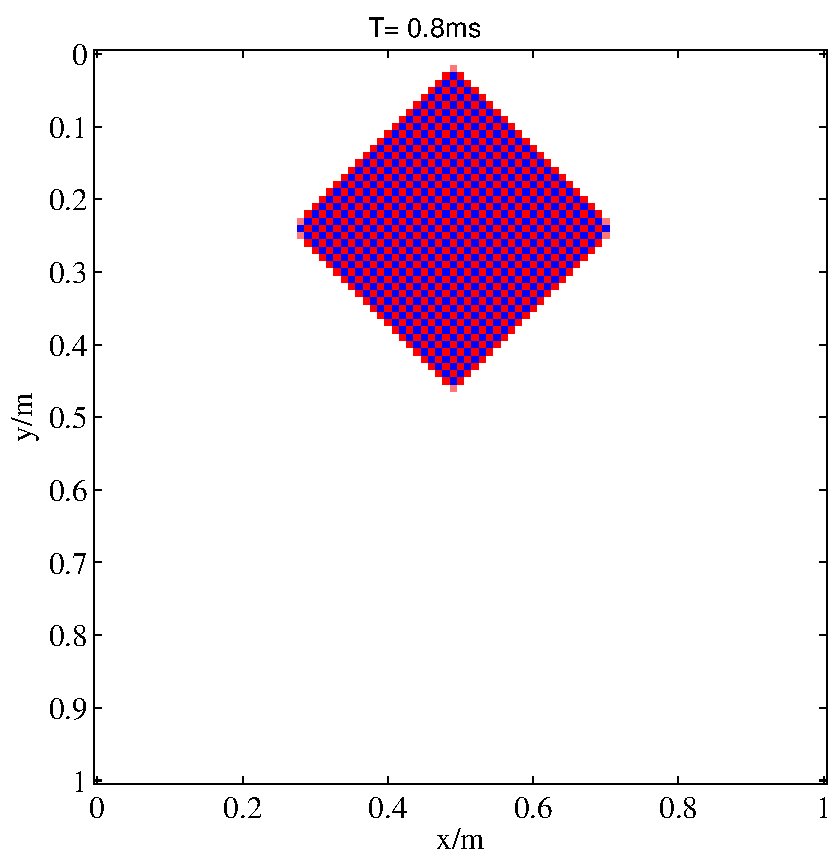
\includegraphics[width=\textwidth]{figures/courandt_1.pdf}
        \caption{}
    \end{subfigure}
    \hfill
    \begin{subfigure}[b]{0.45\textwidth}
        \centering
        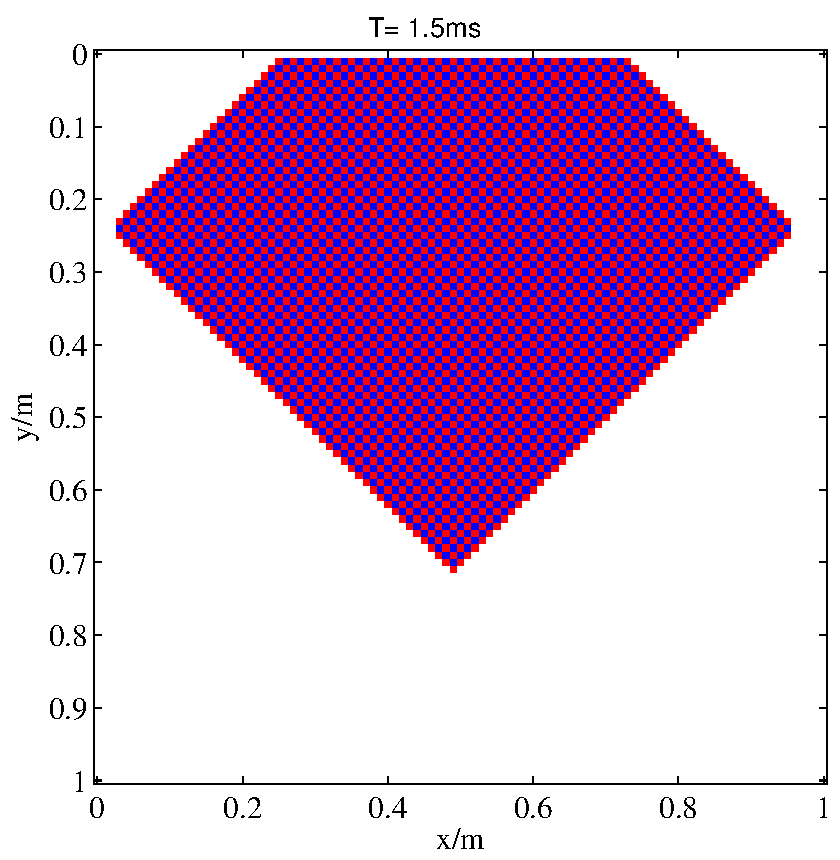
\includegraphics[width=\textwidth]{figures/courandt_2.pdf}
        \caption{}
    \end{subfigure}
    \vfill
    \begin{subfigure}[b]{0.45\textwidth}
        \centering
        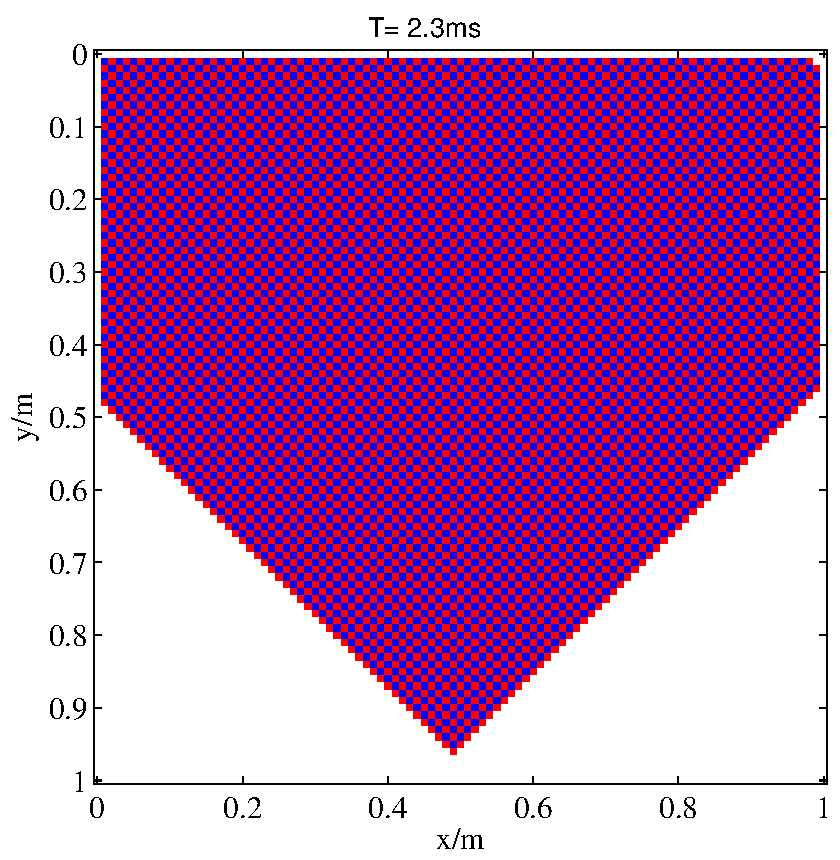
\includegraphics[width=\textwidth]{figures/courandt_3.pdf}
        \caption{}
    \end{subfigure}
    \hfill
    \begin{subfigure}[b]{0.45\textwidth}
        \centering
        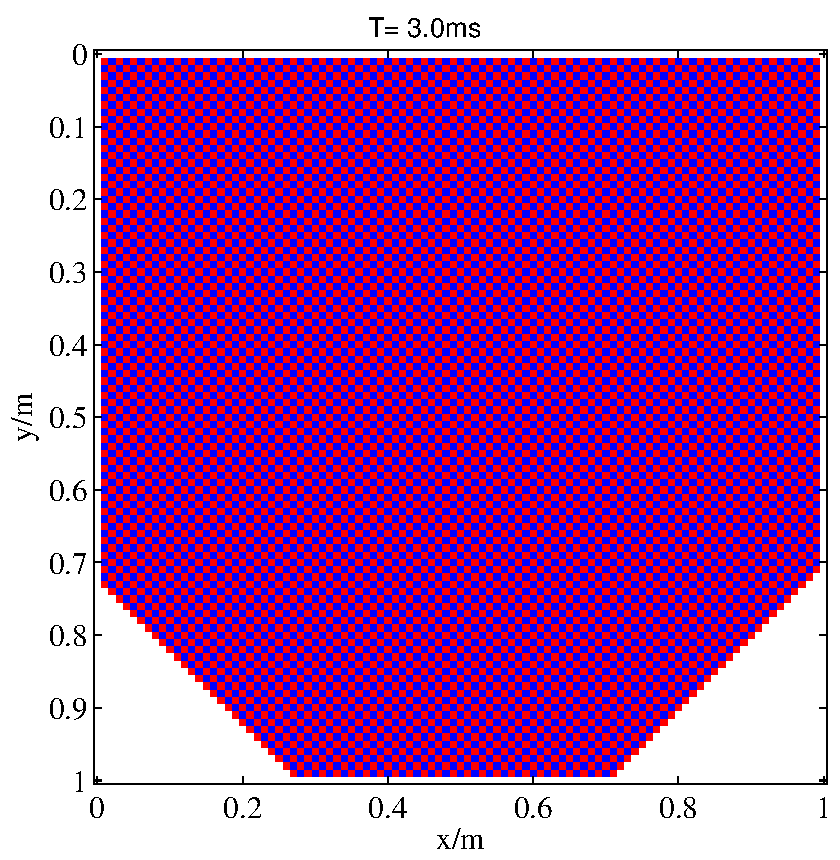
\includegraphics[width=\textwidth]{figures/courandt_4.pdf}
        \caption{}
    \end{subfigure}
    \caption{\label{courant_pics} Temporal evolution of the Courant instability. In the colored areas the wave amplitudes are extremely large.}
\label{fig_courant}
\end{figure}

\begin{table}[hbt]
\caption{\label{courant.1} The factor $h$ in the Courant criterion for different orders (2nd-12th) and types (Taylor and Holberg) of FD operators.}
\centering
\begin{tabular}{c|c|c}
\textbf{FDORDER} & \textbf{h (Taylor)}      & \textbf{h (Holberg)} \\ \hline
2nd   &   1.0             &  1.0        \\
4th   &   7/6             &  1.184614   \\
6th   &   149/120         &  1.283482   \\
8th   &   2161/1680       &  1.345927   \\
10th  &   53089/40320     &  1.387660   \\
12th  &   1187803/887040  &  1.417065    
\end{tabular}
\end{table} 

% \section{Example problem: homogeneous block model}
% \label{example}

% \subsection{Preliminary considerations}
% To illustrate the usage of \texttt{SOFI2D}, we use a homogeneous block model. The material parameters of the block are: P-wave velocity $V_P=\SI{3369}{m/s}$, S-wave velocity $V_S=\SI{1643}{m/s}$ and density $\rho=\SI{2000}{kg/m^3}$. A point-force source in the vertical direction is located inside the model at point $x_s=\SI{398}{m}$ and $y_s=\SI{398}{m}$}. The source function is a Ricker wavelet (see Chapter \ref{sources}) with a center frequency $f_c=\SI{5}{Hz}$. To calculate the dimensions of the grid the spatial grid spacing is estimated using the grid dispersion criterion. \textcolor{red}{For a 4th order Holberg FD operator using $V_{S,min}=\SI{1643}{m/s}$, $f_{max}=2 \cdot f_c=\SI{10}{Hz}$ and $n=...$ we get:}
% \begin{equation}
%     \Delta h \le \frac{V_{s,min}}{n\; f_{max}} = ...\;\mathrm{m}\;.
% \end{equation}
% \textcolor{red}{The whole model grid has the dimensions 400 x 400 gridpoints}. To avoid a violation of the Courant criterion the time step size $\Delta t$ is calculated according to using $V_{P,min}=\SI{3369}{m/s}$, $h=1.0$ and $\Delta h=\SI{0}{m}$:
% \begin{equation}
%     \Delta t \le \frac{\Delta h}{h \sqrt{2} v_{p,max}} = ... \times 10^{-3} s \approx ...\; \mathrm{ms}\;.
% \end{equation}
% \textcolor{red}{The modeling covers a time span of \SI{5.0}{s}, so about $NT=$ 649 time steps are needed. A line of 100 geophones is placed between $x_{start}=\SI{54}{m}$ and $x_{end}=\SI{5400}{m}$ and a constant depth of $y=\SI{2106}{m}$.} 

% \textcolor{red}{Attenuation parameters: $Q_P=Q_S=\SI{8}{}$.}

% \textcolor{red}{Anisotropic parameters: $\epsilon=\SI{0.26}{}$, $\delta=\SI{-0.05}{}$, $\theta=\SI{30}{}$.}

\section{Definition of the modeling parameters}
\label{modelgeom}
The geometry of the FD grid and all parameters for the wavefield simulation have to be defined in a parameter file (which we name in this case \texttt{sofi2D.json}). In the following we will explain all input parameters in detail.
%%\input{sofi2D.json}
All lines in the parameter file are formated according to the JSON standard~(\url{http://www.json.org}) and organized as 
\begin{verbatim}
"VARNAME" = "Parameter value",
\end{verbatim}
where a comment line can look like this:
\begin{verbatim}
"Comment" = "This is a useful comment",
"3D Grid information" = "comment",
\end{verbatim}
Here, \texttt{VARNAME} is a symbolic name for the actual different parameters shown below. Basically, all non-JSON conforming lines will be ignored. The order of the various parameters does not matter, but we typically group parameters that belong together. If critical parameters are missing, the code will stop and an error message will appear. The program outputs the read and all updated/adjusted and possibly calculated parameters unless such output is suppressed.

\subsection{Domain decomposition}
\begin{verbatim}
"Domain Decomposition" : "comment",
            "NPROCX" : "4",
            "NPROCY" : "2",
\end{verbatim}

with

\texttt{NPROCX} : number of (MPI) processors in x-direction\\
\texttt{NPROCY} : number of (MPI) processors in y-direction

\begin{figure}[ht!]
\centering
    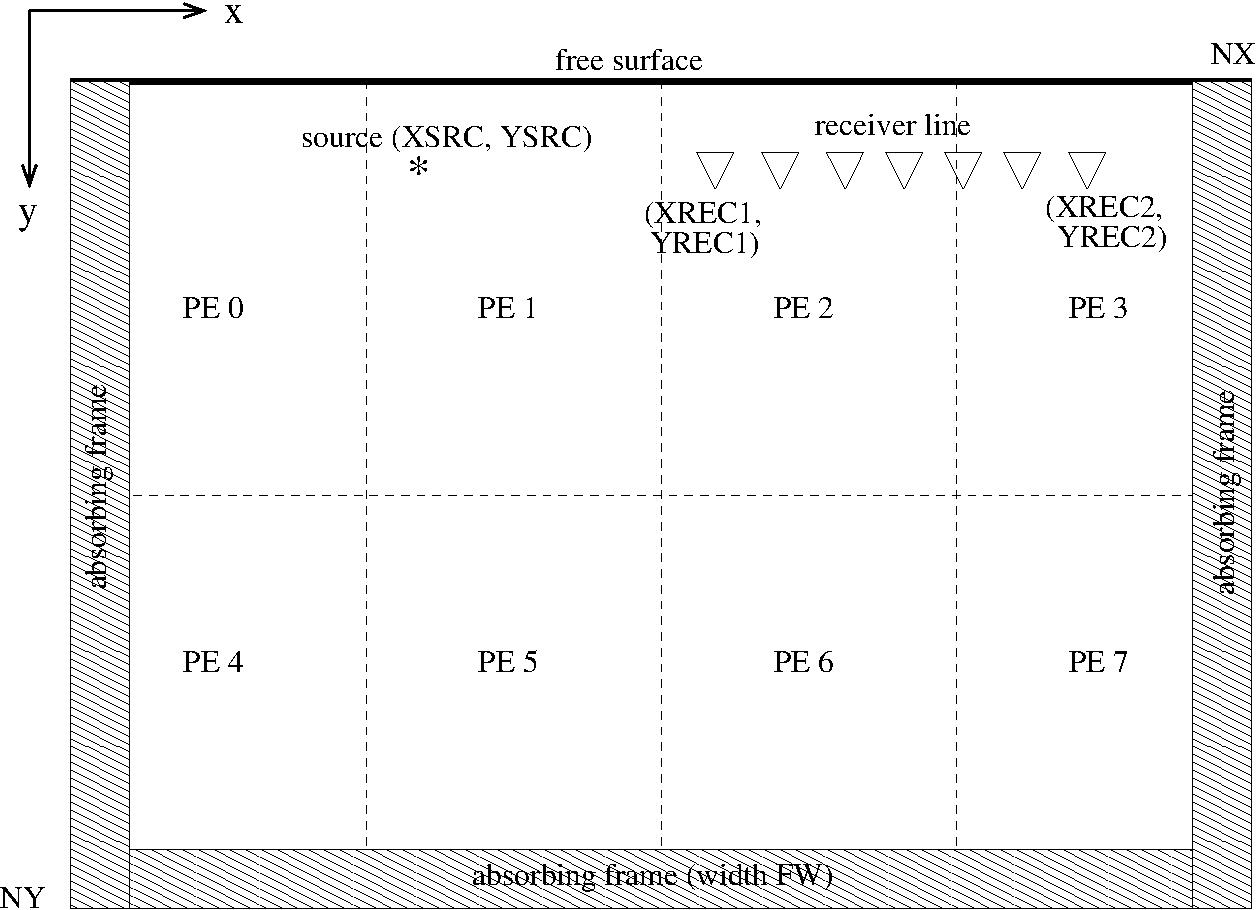
\includegraphics[width=12cm,angle=0]{figures/grid.pdf}
    \caption{Geometry of the numerical FD grid using 4 processors in the $x$-direction (\texttt{NPROCX=4}) and 2 processors in the $y$-direction (\texttt{NPROCY=2}). At the top of the numerical mesh, the PEs apply a free surface boundary condition if \texttt{FREE\_SURF}=1, otherwise an absorbing boundary condition is used; the width of the absorbing frame is \texttt{(FW-1)*DH} in meters. The size of the total grid is \texttt{NX} grid points in the $x$-direction and \texttt{NY} gridpoints in the $y$-direction. The origin of the Cartesian coordinate system is at the top left corner of the grid, i.e., the first upper-left grid point corresponds to coordinate $x=0$, $y=0$.}
\label{fig_grid}
\end{figure}

Parallelization is based on domain decomposition (see Fig.~\ref{fig_grid}), i.e., each processing element (PE) updates the wavefield within its portion of the grid. The model is decomposed by the program into subgrids (blocks). After decomposition, each processing elements (PE) saves only its sub-volume of the grid. \texttt{NPROCX} and \texttt{NPROCY} specify the number of (MPI) processors in horizontal and vertical direction, respectively (Fig.~\ref{fig_grid}). Thus, the total number of processors is \texttt{NP=NPROCX*NPROCY}; this values must be specified when starting the program with the following command: \texttt{mpirun -np $<$NP$>$ ../bin/sofi2D sofi2D.json}. If the total number of processors in \texttt{sofi2D.json} and the number of MPI processes differ, the program will terminate immediately with a corresponding error message. Obviously, the total number of PEs (\texttt{NPROCX*NPROCY}) used to decompose the model should be less or equal the total number of CPU cores available on your parallel processing machines or cluster. You can oversubscribe compute nodes but this usually hurts performance. In order to reduce the amount of data transferred between PEs, one should try to realize more or less cubic subgrids. In our example, we use 4 PEs in horizontal direction (\texttt{NPROCX=4}) and 2 PEs in vertical direction (\texttt{NPROCY=2}). The total number of PEs used by the program, and hence the number of MPI processes, is \texttt{NP=NPROCX*NPROCY=8}.

\subsection{Order of the FD operator}
\begin{verbatim}
"FD order" : "comment",
            "FDORDER" : "4",
            "FDORDER_TIME" : "2",
            "MAXRELERROR" : "1",
\end{verbatim}

with

\texttt{FDORDER} : order of the spatial FD operator (2, 4, 6, 8, 10 or 12)\\
\texttt{FDORDER\_TIME} : order of the temporal FD operator (2 or 4)\\
\texttt{MAXRELERROR} : Maximum relative group velocity error (Taylor=0; Holberg=1)

\texttt{FDORDER\_TIME}=2 correspondents to the classical leapfrog scheme and \texttt{FDORDER\_TIME}=4 to a fourth order accurate scheme. By the option \texttt{MAXRELERROR}, you can switch between Taylor and Holberg FD coefficients but also define a maximum of tolerated group velocity error in percent (Taylor coefficients=0, Holberg coefficients: 1 for $E=0.1\%$, 2 for $E=0.5\%$, 3 for $E=1.0\%$, and 4 for $E=3.0\%$). The chosen FD operator and FD coefficients have an influence on the numerical stability and grid dispersion (see next section).

\subsection{Space discretization}
\begin{verbatim}
"2-D Grid" : "comment",
            "NX" : "400",
            "NY" : "400",
            "DH" : "2.0",
\end{verbatim}

with

\texttt{NX} : number of grid points in the $x$-direction \\
\texttt{NY} : number of grid points in the $y$-direction\\
\texttt{DH} : distance between grid points in both spatial directions (grid size in meters)

These lines specify the size of the total grid (Fig.~\ref{fig_grid}) and therefore the size of external models. An equidistant grid is used in the FD software. The size of the total grid in $x$-direction is \texttt{(NX-1)*DH} and in $y$-direction \texttt{(NY-1)*DH}. \textbf{Note that the $y$-direction always corresponds to the vertical direction} (i.e., to depth). \texttt{NX/NPROCX} and \texttt{NY/NPROCY} must be integer values (for the time being, i.e., subdomains must have equal sizes -- this will be changed in a future version of the program).

To avoid numerical dispersion, the wavefield must be discretized with a certain number of grid points per wavelength. The number of grid points per wavelength depends on the order of the spatial FD operators used in the simulation. The criterion to avoid numerical dispersion is shown in eq.~\ref{eq:dh}; the program assumes that the maximum frequency of the source signal is approximately two times the center frequency. To avoid numerical dispersion of body waves, 8 grid points per minimum wavelength ($N=8$) are necessary for a fourth order algorithm and $N=12$ grid points for a second order algorithm (Table~\ref{grid_disp.2}. The dispersion criterion is checked by the FD software. See the SOFI2D log for further information or warnings. Please note that the FD code will not terminate due to grid dispersion.

\subsection{Time stepping}
\begin{verbatim}
"Time Stepping" : "comment",
			"TIME" : "0.5",
			"DT" : "1.0e-4",
\end{verbatim}

with

\texttt{TIME} : propagation time of seismic waves in the entire model (in seconds)\\
\texttt{DT} : time stepping interval (in seconds)

The time stepping interval $DT$ has to fulfill the stability criterion in eq.~\ref{courant_crit}, which is checked for the entire model. If the criterion is violated, the FD program will terminate with a corresponding error message. The maximum value for $DT$ at the stability limit is output, so you may simply try a certain $DT$, start the program, and then check what the program suggests as time step interval.

\subsection{Wave equations}
The parameter \texttt{WEQ} specifies the type of wave equation to use for modelling. Example:
\begin{verbatim}
"Wave Equation" : "comment",
            "WEQ" : "VEL_TTI",
\end{verbatim}
This parameter is given as string and can have the following values:
\begin{itemize}
\item \textbf{AC\_ISO}: acoustic isotropic wave equation
\item \textbf{VAC\_ISO}: viscoacoustic isotropic wave equation
\item \textbf{EL\_ISO}: elastic isotropic wave equation
\item \textbf{EL\_VTI}: elastic VTI wave equation
\item \textbf{EL\_TTI}: elastic TTI wave equation
\item \textbf{VEL\_ISO}: viscoelastic isotropic wave equation
\item \textbf{VEL\_VTI}: viscoelastic VTI wave equation
\item \textbf{VEL\_TTI}: viscoelastic TTI ave equation
\end{itemize}
The type of wave equation specified for \texttt{WEQ} determines which model files are read from disk and whether Q-related parameters are required, etc. Note that at the time of writing this manual not all wave equations have been implemented yet.

\subsection{Sources}
\label{sources}
\begin{verbatim}
"Source" : "comment",
            "SOURCE_SHAPE" : "1",
            "SIGNAL_FILE" : "signal_mseis.tz",
            "SIGOUT" : "0",
            "SIGOUT_FILE" : "./sources/signal_out01",
            "SIGOUT_FORMAT" : "1",
            "SOURCE_TYPE" : "3",
            "SOURCE_TOPO" : "0",
            "SRCREC" : "1",
            "SOURCE_FILE" : "./sources/source.dat",
            "RUN_MULTIPLE_SHOTS" : "0",
            "PLANE_WAVE_DEPTH" : "2106.0",
            "PLANE_WAVE_ANGLE" : "0.0",
            "TS" : "0.2",
\end{verbatim}

with

\texttt{SOURCE\_SHAPE} : shape of source-signal (Ricker=1; Fuchs-M\"uller wavelet=2; from \texttt{SIGNAL\_FILE}=3; sin$^3$=4; Berlage=5; Klauder=6)\\
\texttt{SIGNAL\_FILE} : external signal file name\\
\texttt{TS} : duration of the source-signal (in seconds)

Five built-in wavelets for the seismic source are available. The corresponding time functions are defined in \texttt{src/wavelet.c}. You may modify the time functions in this file and recompile to include your own analytical wavelet or to modify the shape of the built-in wavelets.

\textbf{Ricker wavelet}:
\begin{equation}
    A_r(\tau)= \left(1-2\tau^2\right)\exp(- \tau^2) \quad \mbox{with} \quad \tau=\frac{\pi(t-1.5/f_c-t_d)}{1.0/f_c}\;. 
    \label{eq_ricker}
\end{equation}

\textbf{Fuchs-M\"uller wavelet}:
\begin{equation}
    A_{fm}(t) = \begin{dcases} \sin(2\pi(t-t_d)f_c)-0.5\sin(4\pi(t-t_d)f_c)\,, & t\in[t_d,t_d+1/fc] \\
                 0\,, & \text{otherwise} \end{dcases}\;.
    \label{eq_fm}
\end{equation}

$\mathbf{sin^3}$ \textbf{wavelet}:
\begin{equation}
    A_{s}(t)=\begin{cases} \frac{3}{4} \pi f_c \sin(\pi(t+t_d)f_c)^3\,, & t \in[t_d,t_d+1/fc]\\
           0\,, & \text{otherwise} \end{cases}\;.
\label{eq_s3}
\end{equation}

\textbf{Berlage wavelet} (after \cite{aldrige:90}):
\begin{equation}
    A_b(t)=(t-t_d)^n\,e^{-\alpha (t-t_d)} \cos(2 \pi f_c (t-t_d) + \phi_0)\;.
    \label{eq_berlage}
\end{equation}

\textbf{Klauder wavelet} (after \cite{neelima:18}):
\begin{equation}
\begin{split} A_k(\tau) &= \Re \left\{ \frac{\sin\left(\pi k(\tau-t_d)\,(t_\text{sweep}-\tau+t_d)\right)}{ \pi k (\tau-t_d) e^{2 \pi i f_c (\tau-t_d)} } \right\} \\
\mbox{with} \quad k &= \frac{f_\text{max}-f_\text{min}}{t_\text{sweep}}\;,\quad\tau = t-\frac{n_\text{twidth}}{f_c}\quad\text{and}\quad f_c=\frac{f_\text{max}+f_\text{min}}{2}.\end{split}
    \label{eq_klauder}
\end{equation}

In these equations $t$ denotes time and $f_c$ is the center frequency. It is specified in the \texttt{SOURCE\_FILE} either directly, or for the Klauder wavelet calculated as half of $f_\text{max}+f_\text{min}$. If parameters are not provided through an external \texttt{SOURCE\_FILE} (\texttt{SRCREC=2}), the center frequency is derived through $f_c=1/TS$. $t_d$ is a time delay which can be defined for each source position in SOURCE\_FILE. Variable time delays for different sources locations allow the simulation of passive acoustic emission. Note that the symmetric (zero-phase) Ricker and Klauder signals are always delayed by $1.5/f_c$ for Ricker, and a shift of $n_\text{twidth}/f_c$ for Klauder, where $n_\text{twidth}$ is half the width of the wavelet in center periods. The Klauder wavelet is tapered on the first and last \qty{20}{\percent} with a cosine taper function. This means that for these two cases the maximum amplitude is excited at the source location after one and a half or $n_\text{twidth}$ centre periods, respectively. All source wavelets and the corresponding amplitude spectra for a center frequency of $f_c=\qty{50}{\hertz}$ and a delay of $t_d=0$ are plotted in Fig.~\ref{fig_source_wavelets}. Note the delay of the Ricker and Klauder signal described above. The Fuchs-M\"uller wavelet has a slightly higher center frequency and covers a broader frequency range. The Klauder wavelet covers a frequency range of \qty{10}{\hertz} to \qty{90}{\hertz} and uses a sweep duration of \qty{7}{\second} and $n_\text{twidth}$ of 5 center periods. For the Berlage wavelet, the additional parameters were set to $n=1.5$, $\alpha=210$, and $\phi_0=\qty{-90}{\degree}$.

\begin{figure}
\centering
    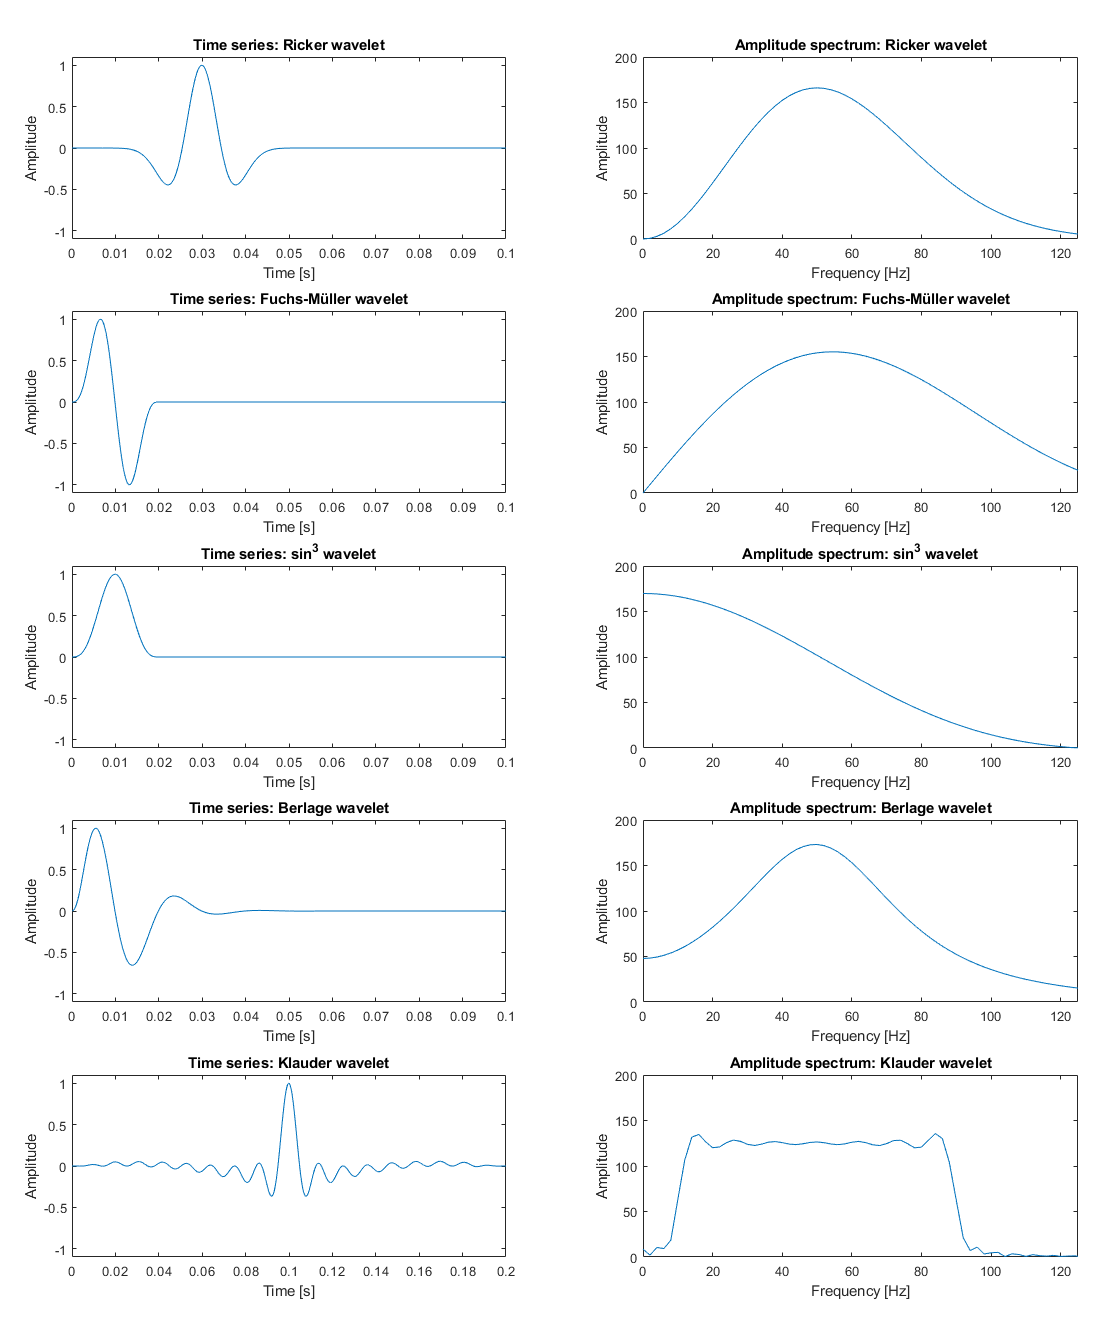
\includegraphics[width=0.9\textwidth]{figures/signals.png}
    \caption{Plot of built-in source wavelets for a center frequency of $f_c=\SI{50}{Hz}$ ($TS=1/f_c=\SI{0.02}{s}$): Ricker signal (1\textsuperscript{st} row), Fuchs-M\"uller signal (2\textsuperscript{nd} row), $sin^3$-signal (3\textsuperscript{rd} row), Berlage signal (4\textsuperscript{th} row), Klauder signal (5\textsuperscript{th} row). Time function (left column) and amplitude spectrum (right column).}
\label{fig_source_wavelets}
\end{figure}

You may also use your own digitized time function as the source wavelet (for instance the signal of the first arrival recorded by a geophone at near offsets). Specify \texttt{SOURCE\_SHAPE=3} and save the samples of your source wavelet in ASCII-format in \texttt{SIGNAL\_FILE}; this file should have a file suffix \texttt{.dat}, \texttt{.txt} or \texttt{.asc}. \texttt{SIGNAL\_FILE} should contain one sample (amplitude value) per line and have the following form:
\begin{verbatim}
# DT=0.0001
0.0
0.01
0.03
...
\end{verbatim}

The time interval between the samples must equal the time step interval (\texttt{DT}) of the FD simulation (see above)! It is therefore often necessary to resample/interpolate a given source time function with a smaller sample rate.

The ASCII file may contain a comment line in the beginning where the sampling interval can be specified as \texttt{DT=<value>} with the value being in seconds. This allows the program to cross-check that the FD time step interval matches the signature time sampling interval and the user does not accidentally modify \texttt{DT} in the parameter file without also updating the sampling interval of the source signature. If the aforementioned comment line is missing in the ASCII file, no cross-check is performed. In case of a mismatch, the program will abort.

The source signature can also be provided as SU-formatted file containing once trace (additional traces will be ignored). In this case, \texttt{SIGNAL\_FILE} should have the file suffix \texttt{.su}. Just like models in SU format, this file needs to use 32-bit native floats. The SU header \texttt{delrt} must be zero (signatures starting at non-zero times are not supported). The SU header \texttt{dt} (in microseconds), if given and greater than 0, is converted to seconds and then cross-checked against the FD time step interval. In case of a mismatch, the program will abort. Note that there is never an automatic interpolation performed by the program (neither when reading ASCII nor when reading SU files).

\texttt{SIGOUT} : output source wavelet (yes=1; no=0)\\
\texttt{SIGOUT\_FILE} : external signal file name for output\\
\texttt{SIGOUT\_FORMAT} : supported output formats (SU=1; ASCII=2; BINARY=3)

The wavelet can be output for quality control purpose by setting \texttt{SIGOUT} to 1 (default value is 0, i.e., no output). This works for both internally generated wavelets based on the parameters provided in \texttt{SOURCE\_FILE} and for externally provided wavelets read from \texttt{SIGNAL\_FILE}. In case QC output is requested, a basename for the output file has to be provided (\texttt{SIGOUT\_FILE}) and an output format (\texttt{SIGOUT\_FORMAT}).

\texttt{SOURCE\_TYPE} : source type (explosive=1; force in $x$-direction=2; force in $y$-direction=3; custom force=4)

\texttt{SOURCE\_TYPE=1} is equivalent to an explosive source that excites P-waves only radiating with the same amplitude into all directions. \texttt{SOURCE\_TYPE}=2 and \texttt{SOURCE\_TYPE}=3 simulate point forces in the $x$- and $y$-directions, respectively. With \texttt{SOURCE\_TYPE}=4, a source in a user-defined direction can be chosen which is defined by the parameter \texttt{SOURCE\_AZIMUTH} specified in in the \texttt{SOURCE\_FILE} (see Fig.~\ref{fig_source_azimuth}). These sources have specific radiation characteristics and excite both P- and S-waves. In case of an explosive source the diagonal components of the stress tensor are assigned with the source wavelet. In case of a directive force in the $x$- or $y$-directions, respectively, the corresponding external body force component ($f_i$, see Eq. 11 of \citep{bohlen:02} is assigned with the source wavelet amplitudes. Please not, that due to the 2D FD scheme, a point force is physically described as a line source. The excited wavefield is therefore not directly comparable to a 3D wave propagation. For 1D media, there is a 2D-to-3D conversion of both body and surface waves.
\begin{figure}[ht!]
\centering
    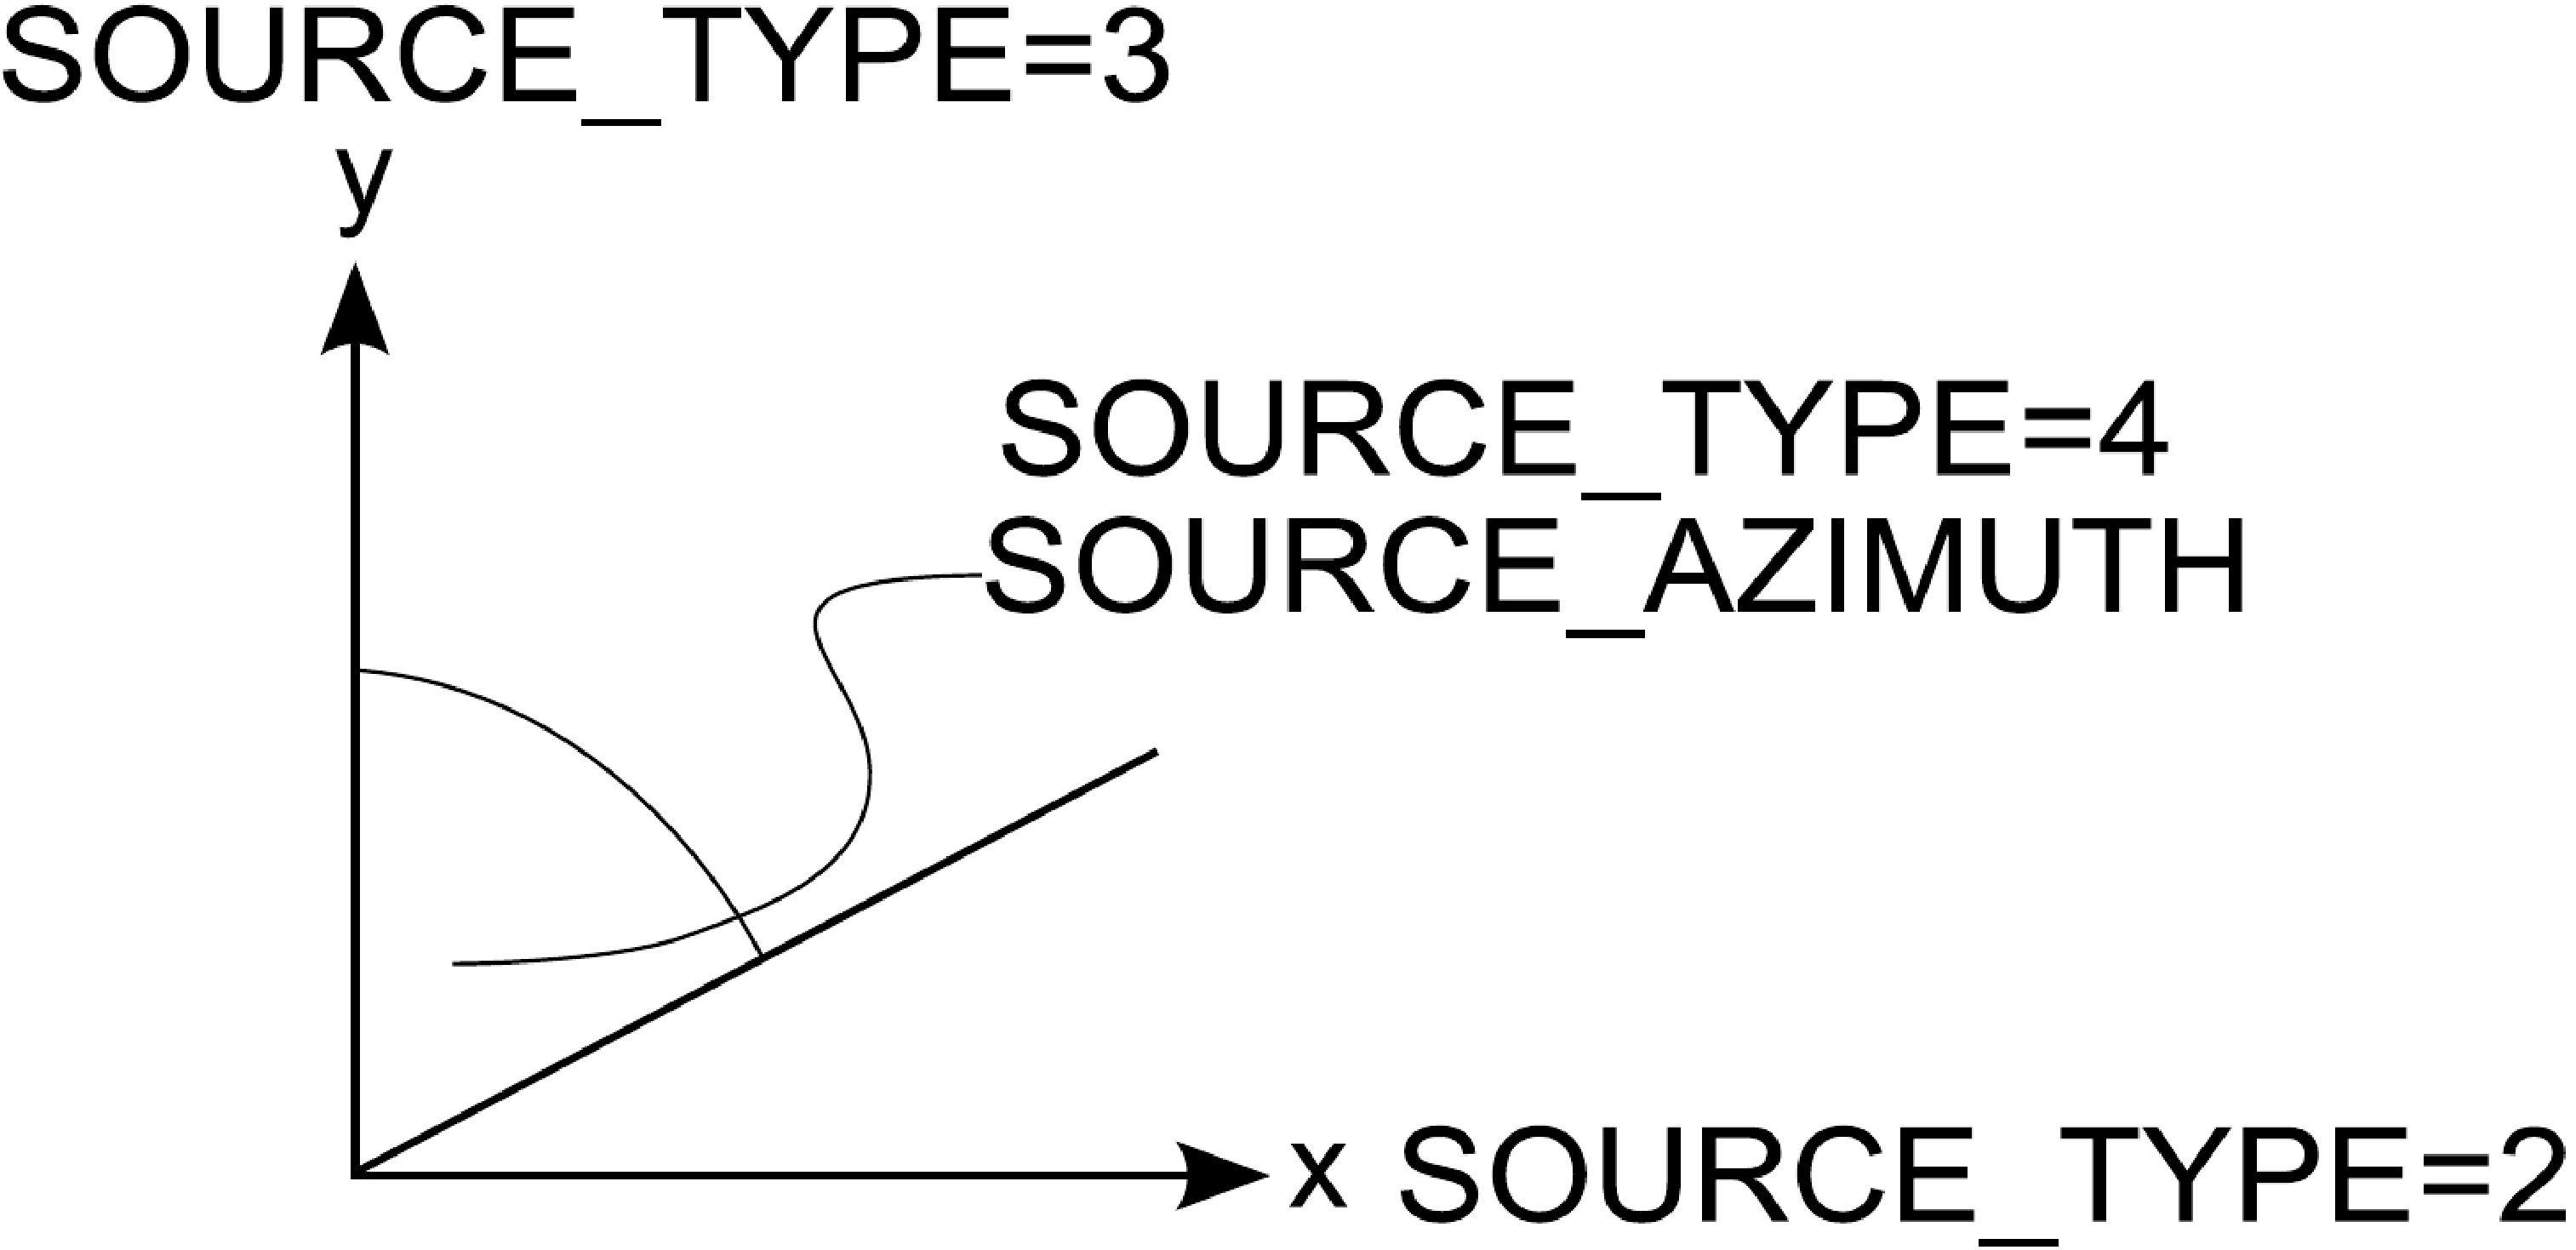
\includegraphics[width=7cm,angle=0]{figures/source_azimuth.pdf}
    \caption{Scheme for \texttt{SOURCE\_TYPE}=4. The parameter \texttt{SOURCE\_AZIMUTH} denotes the angle between the vertical $y$- and horizontal $x$-coordinate.}
    \label{fig_source_azimuth}
\end{figure}

\texttt{SOURCE\_TOPO} : place sources relative to topography (=1) or at absolute depth (=0)

The \texttt{SOURCE\_TOPO} option is only relevant in case sources are read from a file (\texttt{SRCREC}=1). Under normal circumstanes, i.e., when \texttt{SOURCE\_TOPO}=0 which is also the default, sources are placed at the absolute depth specified in the external source file given by \texttt{SOURCE\_FILE}. However, sometimes an explicit air layer is part of the model in case the Earth has topography. When \texttt{SOURCE\_TOPO}=1, then sources are not placed at an absolute depth value but the depth specified in the external source file becomes a depth below topography. The topography is determined by opening the P-wave velocity model and scanning each trace from top to bottom until a change of the first P-wave velocity value that was read in is found (this usually is the interface between air and the solid Earth). The actual P-wave velocity value of the first (air) layer itself does not matter, we only scan for a change. Example: if you would like to simulate sources in 12\;m deep shot holes along a free surface with topographic variations, you need an explicit air layer in the model, you need to set the depth of the source (YSRC, see below) to "12.0" in the external source file, and you finally need to switch on the \texttt{SOURCE\_TOPO} option.

\texttt{SRCREC} : read source positions (from external \texttt{SOURCE\_FILE}=1; from internal \texttt{PLANE\_WAVE}=2)\\
\texttt{SOURCE\_FILE} : external source file name

A source file should have the following format:
\begin{verbatim}
XSRC     YSRC     TD     FC     AMP      SOURCE_AZIMUTH     SOURCE_TYPE
\end{verbatim}

where

\texttt{XSRC} : $x$-coordinate of a source point (in meters)\\
\texttt{YSRC} : $y$-coordinate (depth) of a source point (in meters)\\
\texttt{TD} : time-delay for the source point (in seconds)\\
\texttt{FC} : center frequency of the source signal (in Hz)\\
\texttt{AMP} : maximum amplitude of the source signal

Optional parameters:\\
\texttt{SOURCE\_AZIMUTH} : If \texttt{SOURCE\_TYPE}=4, it represents the angle in degrees between the $y$- and $x$-directions; a \texttt{SOURCE\_AZIMUTH}=0 corresponds to the case \texttt{SOURCE\_TYPE}=3 and \texttt{SOURCE\_AZIMUTH}=90 corresponds to \texttt{SOURCE\_TYPE}=2 (please note that there is a numerical inaccuracy between \texttt{SOURCE\_TYPE}=2 and its analog version \texttt{SOURCE\_AZIMUTH}=90)\\
\texttt{SOURCE\_TYPE} : If \texttt{SOURCE\_TYPE} is set here, the value of \texttt{SOURCE\_TYPE} in the input file is ignored

\texttt{RUN\_MULTIPLE\_SHOTS} : multiple shots (modeled simultaneously=0; modeled individually=1)

This parameter defines if multiple shots are modeled simultaneously or whether each shot is modeled individually. If the parameter is set to 0, multiple sources are modeled together. If more than one source is defined in \texttt{SOURCE\_FILE}, each source is triggered at the same time. For \texttt{RUN\_MULTIPLE\_SHOTS}=1, every source specified in the \texttt{SOURCE\_FILE} is modeled individually. The \texttt{SEIS\_FILE} name then contains the number of the shot, e.g., \texttt{test\_vx.su.shot1.0}.

\texttt{PLANE\_WAVE\_DEPTH} : Depth of plane wave excitation (in meters)\\
\texttt{PLANE\_WAVE\_ANGLE} : Dip of plane wave from vertical (in degrees)

In some applications, e.g., transmission experiments or the simulation of teleseismic events, the generation of plane waves are required. If you specify a \texttt{PLANE\_WAVE\_DEPTH}>0, a plain wave at a depth of \texttt{PLANE\_WAVE\_DEPTH} is excited. In the case of \texttt{PLANE\_WAVE\_DEPTH}<0, point sources are applied; thus, \texttt{SRCREC} should be set to 1, otherwise no sources are applied. The plane wave is simply generated by applying the source time function (\texttt{SOURCE\_SHAPE}) with the source characteristic (\texttt{SOURCE\_TYPE}) at each grid point along a straight line (2D modeling). You can also excite plane waves with a certain dip from the vertical direction. See Fig.~\ref{fig_plane_wave} for a description of the geometry for the generation of dipping plane waves. In case of plane waves, the duration of the source signal, and hence the center frequency of the source (\texttt{1/TS}), is specified by $TS$ in the parameter file. In case of point sources (\texttt{PLANE\_WAVE\_DEPTH}=0.0 and \texttt{SRCREC}=1) the center frequency is defined in \texttt{SOURCE\_FILE} together with the location and the time delay. In case of point sources, the parameter $TS$ is ignored.
\begin{figure}[ht!]
\centering
    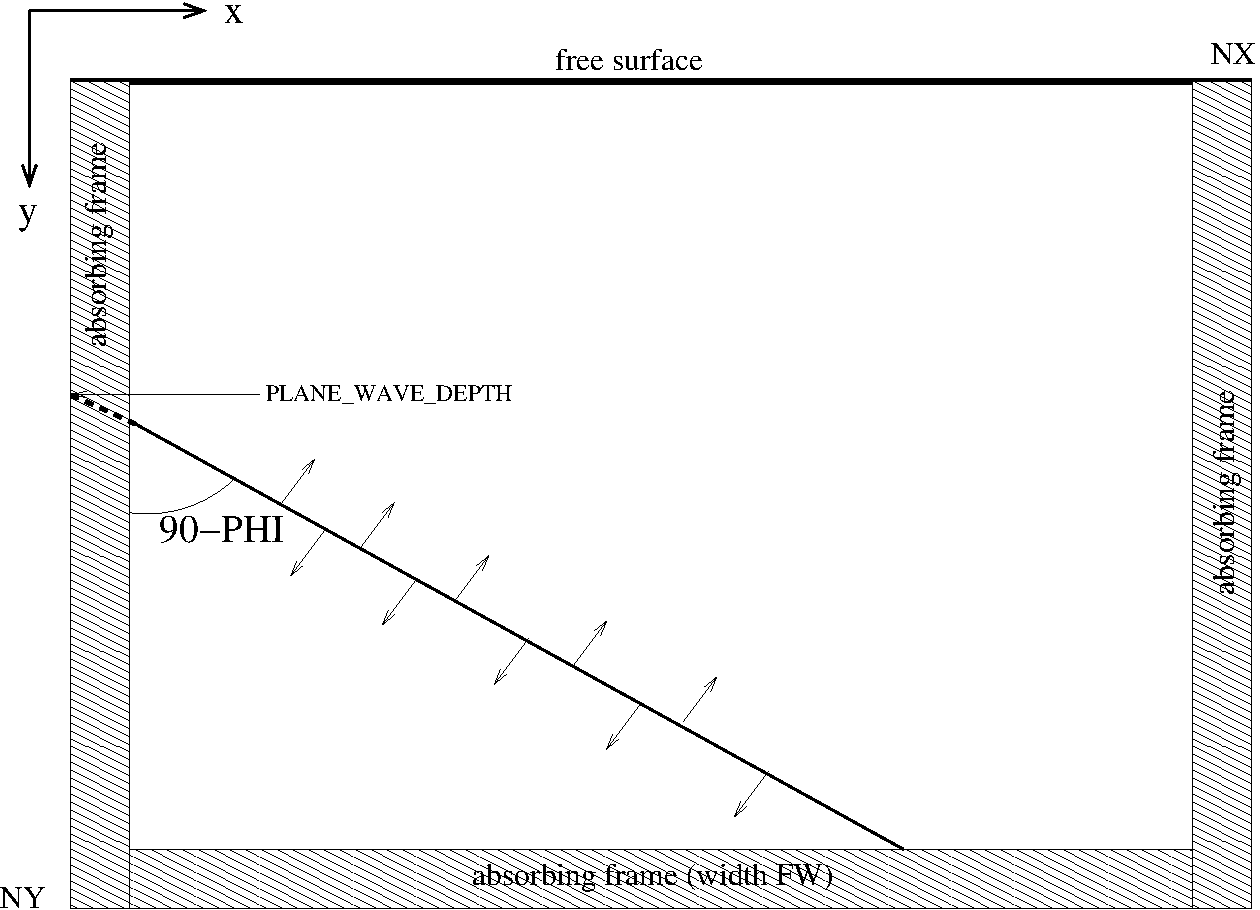
\includegraphics[width=12cm,angle=0]{figures/plane_wave.pdf}
    \caption{Plane waves are generated by assigned source points along  straight lines (2D simulation) or planar planes (3D simulation) with the source wavelet. The parameter \texttt{PLANE\_WAVE\_DEPTH} defines the depth of this line/plane at $x=0$, and the parameter \texttt{PLANE\_WAVE\_ANGLE} specifies the incidence angle with respect to the vertical direction (\texttt{PLANE\_WAVE\_ANGLE}=0 corresponds to vertical incidence).}
    \label{fig_plane_wave}
\end{figure}

\subsection{Generation of models}
\label{gen_of_mod}
\begin{verbatim}
"Model" : "comment",
            "READMOD" : "1",
            "MFILE" : "model/test/TTI_Thomsen_1",
            "WRITE_MODELFILES" : "0",
\end{verbatim}

with

\texttt{READMOD} : read model parameters from \texttt{MFILE} (yes=1; generated \enquote{on the fly}=0)\\
\texttt{MFILE} : basename for the model files, used to read from file and/or to write model for validation\\
\texttt{WRITE\_MODELFILES} : switch on which models are written to file if generated internally \enquote{on the fly} (no model=0; all models=1; only the density model=2).

If \texttt{READMOD}=1, the P-wave, S-wave, and density model grid (if $L=0$, see Chapter~\ref{Q-approximation}) and additionally the attenuation grids (if $L>0$) are read from external files. These files can either be in plain binary format, or SU format -- if SU-formatted files (suffix \texttt{.su}) are present, they will be preferred. Note that the upper left sample of the model (i.e., the first sample on the first trace) is considered to be at Cartesian coordinate $(0,0)$. \texttt{MFILE} defines the basic file name that is expanded by the following extensions: \textbf{P-wave velocity model} \enquote{.vp.su} (or \enquote{.vp}), \textbf{S-wave velocity model} \enquote{.vs.su} (or \enquote{.vs}), both in \SI{}{m/s}, \textbf{density model} \enquote{.rho.su} (or \enquote{.rho}) in \SI{}{kg/m^3}, \textbf{P-wave attenuation model} \enquote{.qp.su} (or \enquote{.qp}), \textbf{S-wave attenuation model} \enquote{.qs.su} (or \enquote{.qs}). In case of anisotropy, the program will also read the \textbf{Thomsen parameter models} \enquote{.epsilon.su} (or \enquote{.epsilon}) and \enquote{.delta.su} (or \enquote{.delta}), and in case of TTI the tilt angle \enquote{.theta.su} (or \enquote{.theta}). The angle is defined as angle in degree against the vertical axis, with positive angles being measured anti-clockwise. A constant zero-degree tilt angle section for TTI corresponds to the VTI case.

In plain binary files, each material parameter value must be saved as 32-bit (4-byte) native float. The fast dimension is the $y$-direction (see, e.g., \texttt{src/readmod*.c}). The number of samples for the entire model in the $x$-direction is $NX$ and the number of values in the $y$-direction is always $NY$. The file size of each model file thus must be $NX*NY*4$ bytes. You may check the model structure using the SU command \textbf{ximage}: \texttt{ximage n1=$<$NY$>$ n2=$<$NX$>$ $<$ model/test.vp}.

For SU-formatted model files, the set-up is similar. They must use 32-bit native floats. The number of samples per trace must equal $NY$, and the number of traces must equal $NX$. Note: if there are more than $NY$ samples per trace in the SU file, the additional samples per trace will be ignored. That means, the code will only ever read $NY$ samples. The same holds if there are more than $NX$ traces in the file -- the code will only ever read $NX$ traces (starting from the beginning of the file) as specified in the parameter file. In case the entire file is used, it should have size $NX*NY*4+NX*240$ bytes (as the SU tracer header has a length of 240 bytes).

If \texttt{READMOD}=0, the model is generated \enquote{on the fly} by SOFI2D, i.e., it is generated internally before the time loop starts. Note that if \texttt{READMOD}=0, the function building the model is called from within the software and must therefore be specified in the Makefile; you need to re-compile SOFI2D by changing to the \texttt{build} directory and typing \texttt{make all} in case you would like to modify and/or update the internal model generation.

As the variable \texttt{MFILE} is also used to write the internally created model(s), you can specify which models are output (\texttt{WRITE\_MODELFILES}). Be aware that the output of additional models besides density will cause extra (but temporal) memory allocation of the size of the local subgrid times the number of models! 
% The actual $V_p$ and $V_s$ models can be easily calculated from the following relationships:
% \begin{subequations}
%     \begin{align}
%         U &= V_s \cdot V_s \cdot rho\;,\\
%         Pi &= V_p \cdot V_p \cdot rho\;.
%         \label{eq_U_PI}
%     \end{align}
% \end{subequations}
    
\subsection{Q-approximation}
\label{Q-approximation}
\begin{verbatim}
"Q-approximation" : "comment",
            "L" : "1",
            "F_REF" : "50.0",
            "FL1" : "50.0", 
            "TAU" : "0.1",
\end{verbatim}

with 

\texttt{L} : number of relaxation mechanisms (elastic=0; viscoelastic>0; up to 5)\\
\texttt{F\_REF} : reference frequency\\
\texttt{FL1} : relaxation frequencies (one for each relaxation mechanism; \texttt{FL2,...,FL5})\\
\texttt{TAU} : ratio of strain-retardation and stress-relaxation times (describes the directional variation of attenuation); only used for internal model generation

These lines are omitted in the elastic version (if \texttt{L}=0). The frequency dependence of the (intrinsic) quality factor $Q(\omega)$ is defined by the \texttt{L} relaxation frequencies (\texttt{FL1}$=f_l=2\pi/\tau_{\sigma l}$). In the current model (see \texttt{model.c}), these values are assigned to all gridpoints for both P- and S-waves. Thus, intrinsic attenuation is homogeneous and equal for P- and S-waves ($Q_p(\omega)=Q_s(\omega)$). However, it is possible to simulate any spatial distribution of absorption by assigning the gridpoints with different $\tau$-values. Note that for a single relaxation mechanism (\texttt{L}=1), $Q \approx 2/\tau$ (\cite{bohlen:02}; $Q(\omega)$ for \texttt{L}=1, \texttt{FL1}$ =f_l=\SI{70}{Hz}$, and \texttt{TAU}$=\tau=0.04$ is shown in Fig. 11). \textcolor{red}{The Matlab script \texttt{/mfiles/qplot.m} can be used to plot $Q(\omega)$ for different values of \texttt{L}, \texttt{FL1}, and \texttt{TAU}}. The script \texttt{qapprox.m} finds optimal values in a way that they fit a desired function $Q(\omega)=$~const in a least-squares sense.

Please note, that due to dispersive media properties the viscoelastic velocity model is only defined for the reference frequency only. In SOFI2D, this reference frequency is specified as the center source frequency. At the exact reference frequency, elastic and viscoelastic models are equivalent. As a consequence, slightly smaller and larger minimum and maximum velocity values occur in the viscoelastic model.

\subsection{Boundary conditions}
\label{abs}
\begin{verbatim}
"Boundary Conditions" : "comment",
            "FREE_SURF" : "0",
            "BOUNDARY" : "0",
            "FW" : "20",
            "ABS_TYPE" : "2",
            "NPOWER" : "4.0",
            "K_MAX_CPML" : "1.0",
            "VPPML" : "3500.0",
            "FPML" : "15.0",
            "DAMPING" : "8.0",
\end{verbatim}

with

\texttt{FREE\_SURF} : free surface at the top of the model (no=0; yes=1)\\
\texttt{BOUNDARY} : periodic boundary condition at edges (no=0; left and right=1)\\ 
\texttt{FW} : width of absorbing frame in grid points (no=0; exponential damping applied at the left/right, front/back, and bottom of the grid>0 - \cite{cerjan:85})\\
\texttt{ABS\_TYPE}: type of absorbing boundary (CPML=1; damping=2)\\
\texttt{NPOWER} : exponent for calculation of damping profile \\
\texttt{K\_MAX\_CPML} : \\
\texttt{VPPML} : attenuation velocity within the PML, approximately the propagation velocity of the dominant wave near the model boundaries (in m/s)\\
\texttt{FPML} : dominant signal frequency (in Hz)

In some cases, it is useful to apply periodic boundary conditions, for example when modeling seismic wave transmission through random media (\cite{bohlen:02}). If \texttt{BOUNDARY}=1 no absorbing boundaries are installed at the left and right sides of the grid. Instead, wavefield information is copied from left to right and vice versa. The effect is, for example, that a wave which leaves the model at the left side enters the model again at the right side.

The convolutional perfectly matched layer (CPML) boundary condition implementation is based on \citet{komatitsch:07} and \citet{martin:09}. A width of the absorbing frame of \texttt{FW}=10-20 grid points should be sufficient. For the optimal realization of the PML boundary condition, you have to specify the dominant signal frequency \texttt{FPML} occurring during the wave simulation; this is usually the center source frequency \texttt{FC} specified in the source file.

\texttt{DAMPING} : attenuation at the edges of the grid (in \%)

With the \texttt{DAMPING} boundary, attenuation is specified at the edges of the numerical grid, i.e., amplitudes are multiplied by a factor of 1-\texttt{DAMPING} at the edges. The width of the absorbing frame should be \texttt{FW}>20 gridpoints (\cite{cerjan:85}); a good choice is 8.0$\%$; for larger values, reflections at the onset of the absorbing frame might occur (\cite{cerjan:85}). In order to avoid such an impedance contrast between the model domain and the absorbing boundary layer, \texttt{FW} should increase and \texttt{DAMPING} should decrease. If \texttt{FREE\_SURF}=0, damping is also applied at the top of the model.

\subsection{Wavefield snapshots}
\begin{verbatim}
"Snapshots" : "comment",
            "SNAP" : "1",
            "TSNAP1" : "0.01",
            "TSNAP2" : "0.5",
            "TSNAPINC" : "0.01",
            "IDX" : "1",
            "IDY" : "1",
            "SNAP_FORMAT" : "3",
            "SNAP_FILE" : "./snap/hh_e_t",
\end{verbatim}

with

\texttt{SNAP} : output of snapshots (no seismograms=0; particle velocities=1; pressure field/hydrophones=2; curl and divergence energy=3; velocities, pressure, and energy=4)\\
\texttt{TSNAP1} : first snapshot (in seconds)\\
\texttt{TSNAP2} : last snapshot (in seconds)\\
\texttt{TSNAPINC} : increment (in seconds; should be a multiple of \texttt{DT})\\
\texttt{IDX} : increment in $x$-direction (grid points)\\
\texttt{IDY} : increment in $y$-direction (grid points)\\
\texttt{SNAP\_FORMAT} : data format (ASCII=2; binary=3)\\
\texttt{SNAP\_FILE} : output basename

If \texttt{SNAP}>0, wavefield information (particle velocities, pressure or curl and divergence of particle velocities) for the entire model is saved on disk; therefore, be sure that you have enough free space! Each PE is writing its sub-volume to disk. The filenames have the basename \texttt{SNAP\_FILE} plus an extension that indicates the PE number in the logical processor array (see Fig.~\ref{fig_grid}). Note that the file sizes increase during the simulation. It may therefore be necessary to reduce the amount of snapshot data by increasing \texttt{IDX} and \texttt{IDY} and/or \texttt{TSNAPINC}. In order to merge the separate snapshot of each PE after the completion of the wave modeling, you can use the program \texttt{snapmerge}.

\subsection{Receivers}
\begin{verbatim}
"Receiver" : "comment",
            "SEISMO" : "0",
            "READREC" : "1",
            "REC_TOPO" : "0",
            "REC_FILE" : "./receiver/receiver.dat",
            "REFRECX, REFRECY" : "0.0 , 0.0",
            "XREC1,YREC1" : "50.0 , 1.0",
            "XREC2,YREC2" : "350.0 , 1.0",
            "NGEOPH" : "1",
\end{verbatim}

with

\texttt{SEISMO} : output of seismograms (no seismograms=0; particle velocities=1; pressure/hydrophones=2; curl and div=3; everything=4)

If \texttt{SEISMO}>0, seismograms are saved on disk; when \texttt{SEISMO} is 1, $x$- and $y$-components of particle velocity will be written according to parameters specified in section~\ref{seismograms}; if \texttt{SEISMO}=2, pressure (sum of the diagonal components of the stress tensor) recorded at the receiver locations is written; if SEISMO=3 the curl and divergence are saved. The curl and divergence of the particle velocities are useful to separate P- and S-waves in the snapshots of the wavefield. SOFI2D calculates the divergence and the magnitude of the curl of the particle velocity field (\cite{dougherty:88}). The motivation for this is as follows: according to \citet{morse:53}, the energy of P- and S-wave particle velocities, respectively, are
\begin{equation}
    E_p=\left(\lambda + 2 \mu\right) \left[ \text{div}(\vec{v}) \right]^2 \quad \mbox{and} \quad E_s=\mu \left|\text{rot}(\vec{v})\right|^2\;,
    \label{eq_E}
\end{equation}
where $\lambda$ and $\mu$ are the Lam\`{e} parameters, and $\vec{v}$ is the particle velocity vector. In order to preserve the divergence and curl sign information  while showing relative compressional and shear particle velocity amplitudes, we plot the following quantities:
\begin{equation}
    \bar{E}_p = \text{sign}(\text{div}\,\vec{v}) E_p^{1/2} \quad \mbox{and} \quad \bar{E}_s= \text{sign}(\text{rot}\,\vec{v}) E_s^{1/2}\;.
    \label{eq_e}
\end{equation}
The magnitudes of $\bar{E}_p$ and $\bar{E}_s$ are proportional to the magnitudes of the P- and S-particle velocities, respectively. Note that interface waves like Rayleigh waves contain both a P- and S-wave component and therefore show up on both quantities of Eq.~\ref{eq_e}.

\texttt{READREC} : read receiver positions from file (from the parameter file=0; from an external file=1)

\texttt{REC\_TOPO} : place receivers relative to topography (=1) or at absolute depth (=0)

The \texttt{REC\_TOPO} option is only relevant in case receivers are read from an external file (\texttt{READREC}=1). Under normal circumstanes, i.e., when \texttt{REC\_TOPO}=0 which is also the default, receivers are placed at the absolute depth specified in the external receiver file given by \texttt{REC\_FILE}. However, sometimes an explicit air layer is part of the model in case the Earth has topography. When \texttt{REC\_TOPO}=1, then receivers are not placed at an absolute depth value but the depth specified in the external receiver file becomes a depth below topography. For details on how the topography is found, please check the \texttt{SOURCE\_TOPO} option.

\texttt{REC\_FILE} : external receiver file name (ASCII-file)\\
\texttt{REFREC} : reference point for receiver coordinate system (if 1, the following 3 parameters are ignored)\\
\texttt{XREC1,YREC1} : position of the first receiver (in meters) \\
\texttt{XREC2,YREC2} : position of the last receiver (in meters)\\
\texttt{NGEOPH} : distance between two adjacent receivers (in grid points)

The locations of the receivers may either be specified in the parameter file or in a separate file (\texttt{REC\_FILE}). When reading them from the parameter file, it is assumed that the receivers are located along a straight line. The first receiver position is defined by (\texttt{XREC1}, \texttt{YREC1}), and the last receiver position by (\texttt{XREC2}, \texttt{YREC2}). The spacing between receivers is \texttt{NGEOPH} grid points; a vertical seismic profile (VSP) is realized when \texttt{XREC1=XREC2} and \texttt{YREC1<YREC2}. When reading from an ASCII-file, each line should contain the receivers coordinates (in meters) as below: the horizontal $x$- and then the vertical $y$-coordinate of each receiver position, respectively.
\begin{verbatim}
50.0   2.0
100.0  2.0
150.0  2.0
...
\end{verbatim}

These receiver coordinates are possibly shifted by \texttt{REFREC}[1] and \texttt{REFREC}[2] into the $x$- and $y$-direction, respectively. This allows for completely moving the receiver spread without modifying \texttt{REC\_FILE}. This may be useful for the simulation of moving profiles in reflection seismics.

Receivers are always located on full grid indices, i.e., a receiver that is located between two grid points will be shifted by the FD program to the closest next grid point. It is not possible to output seismograms for arbitrary receiver locations since this would require a certain wavefield interpolation. It is important to note that the actual receiver positions defined in the \texttt{REC\_FILE} or in \texttt{sofi2D.json} may vary by $DH/2$ due to the staggered positions of the particle velocities and stress tensor components.

\subsection{Receiver array}
\begin{verbatim}
"Receiver array" : "comment",
            "REC_ARRAY" : "0",
            "REC_ARRAY_DEPTH" : "70.0",
            "REC_ARRAY_DIST" : "40.0", 
            "DRX" : "4",
\end{verbatim}

with

\texttt{REC\_ARRAY} : number of receivers in 1D receiver array (no simulation=0)\\
\texttt{REC\_ARRAY\_DEPTH} : depth of first plane (in meters)\\
\texttt{REC\_ARRAY\_DIST} : increment between receiver planes (in meters)\\
\texttt{DRX} : increment between receivers in each plane (in gridpoints)

A horizontal 1D array of receivers is simulated if \texttt{REC\_ARRAY}>0. This option specifies the number of receiver planes horizontal to the surface of the model (parallel to the $x$-axis). The distance between receivers within each plane is \texttt{DRX*DH} (in meters).

\subsection{Seismograms}
\label{seismograms}
\begin{verbatim}
"Seismograms" : "comment",
            "NDT" : "5",
            "SEIS_FORMAT" : "1",
            "SEIS_FILE" : "./su/test_t003",
\end{verbatim}

with

\texttt{NDT} : sampling rate (in FD time steps)

If \texttt{SEISMO}>0, seismograms recorded at the receiver positions are written to the corresponding output files. The sampling rate of the seismograms is \texttt{NDT*DT} seconds. In case of a small time step interval and a large number of time steps, it might be useful to choose a relatively large \texttt{NDT} to avoid an unnecessary detailed sampling of the seismograms and consequently large files of seismogram data.

\texttt{SEIS\_FORMAT} : data output format (SU=1; ASCII=2; binary=3)

It is recommended to use SU (native 4-byte-floats (IEEE on PC)/little endian on PC) format for saving the seismograms. The main advantage of this format is that the time step interval (\texttt{NDT*DT}) and the acquisition geometry (shot and receiver locations) are stored in the corresponding SU header words. Moreover, additional header words like offset are set by SOFI2D. This format thus facilitates a further visualization and processing of the synthetic seismograms. Note, however, that SU cannot handle sampling rates smaller than \SI{1.0e-3}{ms} and the number of samples is limited to about \SI{32000}{}. In such cases, you should increase the sampling rate by increasing \texttt{NDT}. If this is impossible (for example, because the Nyquist criterion is violated), you must choose a different output format (ASCII or binary). 

SU-files can be merged together using the Unix command \texttt{cat}. 

\texttt{SEIS\_FILE} : basename for output of seismograms (\texttt{SEISMO})

Separate seismogram files are output, looking like \texttt{SEIS\_FILE\_vz.su} or \texttt{SEIS\_FILE\_div.bin}. Each PE internally stores seismograms which are recorded in its portion of the grid. After finishing the time step loop, the seismogram parts are internally exchanged and the merged seismograms are collectively saved to the output file. A certain suffix is added to the basename \texttt{SEIS\_FILE} dependent on the chosen \texttt{SEISMO} option (pressure, particle velocity, curl, and divergence). To give an example, the program writes the merged seismograms of the $x$-component of particle velocity to \texttt{SEIS\_FILE\_vx.su}.

\textbf{Wavelet shapes -- practical issues}\\
When using an explosive source, a pressure sensor, and a Ricker wavelet as source function with the standard elastic wave equation, the resulting seismograms have to be integrated one-and-a-half times (\texttt{sufrac power=-1.5}) in order to get back to the original Ricker shape and its spectrum. In addition, there is a polarity reversal due to the definition of pressure; in such a case, the additional parameter \texttt{phasefac=1} would revert the polarity. When using a force source, a velocity sensor, and a Ricker wavelet as source function with the standard elastic wave equation, the resulting seismograms have to be half-integrated (\texttt{sufrac power=-0.5}) in order to get back to the original Ricker shape and its spectrum. There is no polarity reversal.

\subsection{Monitoring the simulation}
\begin{verbatim}
"Monitoring the simulation" : "comment",
            "LOG_FILE" : "log/test.log",
            "LOG" : "0",
            "LOG_VERBOSITY" : "INFO",
            "OUT_TIMESTEP_INFO" : "100",
\end{verbatim}

with

\texttt{LOG\_FILE} : log-file for information about progress of program (each PE is printing log-information to \texttt{LOG\_FILE.MYID})\\
\texttt{LOG} : output of logging information of node (all ranks output to terminal=0; all ranks output to \texttt{LOG\_FILE}=1; rank 0 outputs to terminal and all other ranks to \texttt{LOG\_FILE}=2)

SOFI2D can output a lot of useful and debug information about the modeling parameters and the status of the modeling process. The major part of this information is output by the main MPI process. The \texttt{LOG} parameter in the \texttt{json} file sets the logging output stream. If \texttt{LOG}=0, the main MPI process writes its log to \texttt{stdout}, i.e., on the terminal; this is generally recommended  to monitor the modeling process. You may want to save this screen log to an output file by adding \texttt{2>\&1 | tee sofi2D.jout} to your start command (if you use a queuing system, this output is normally captured anyway and returned by the queuing system at the end of the job). \texttt{LOG}=1 sends all output to log files as specified in the \texttt{json} file. \texttt{LOG}=2 send the output of the main MPI process to \texttt{stdout} and all other ranks write their output to log files.\\

\texttt{LOG\_VERBOSITY} : set how much information is output (\texttt{DEBUG}, \texttt{INFO}, \texttt{WARN}, \texttt{SILENT})

If the parameter is not given, \texttt{LOG\_VERBOSITY} is internally set to \texttt{INFO}, which means the program should output information that is useful for the user. On \texttt{DEBUG} level, additional output (including code line numbers) occurs which can help in debugging issues. On level \texttt{WARN}, only warnings and errors are output, while \texttt{SILENT} means only errors are output -- they cannot be ignored by the user.

\texttt{OUT\_TIMESTEP\_INFO} : time step increment upon which information is output

As the output of information can both slow down the computation for very small models and produce very large log files, you can choose by \texttt{OUT\_TIMESTEP\_INFO} after how many time steps such intermediate information is logged.

% {\subsection{\enquote{On the fly} definition of material parameters}}
% \label{model_def_func}
% If you choose to create the model \enquote{on the fly}, the distribution of the material parameters P-wave velocity $v_p$, S-wave velocity $v_s$, and density $\rho$ for the simple block model has to be defined in the function \texttt{hh\_elastic.c} that can be found in the \texttt{src} folder.

% \begin{verbatim}
% /* -------------------------------------------------------------
%  *   Model homogeneous half space
%  *   if variable "h" is decreased, a layer over half-space is gained
%  *   ------------------------------------------------------------- */

% #include "fd.h"

% void model_elastic(float  **  rho, float **  pi, float **  u){

% 	/*--------------------------------------------------------------------------*/
% 	/* extern variables */

% 	extern int NX, NY, NXG, NYG,  POS[3], MYID;
% 	extern int WRITE_MODELFILES;
% 	extern float DH;
% 	extern char  MFILE[STRING_SIZE];	

% 	/* local variables */
% 	float muv, piv, Vp, Vs, Rhov;
% 	float y;
% 	int i, j, ii, jj;
% 	char modfile[STRING_SIZE];
% 	float ** pwavemod=NULL, ** swavemod=NULL;


% 	/*-----------------material property definition -------------------------*/	

% 	/* parameters for layer 1 */
% 	const float vp1=3500.0, vs1=2000.0, rho1=2000.0, h=100000.0;


% 	/* parameters for layer 2 */
% 	const float vp2=5400.0, vs2=3700.0, rho2=2500.0;


% 	/*-----------------------------------------------------------------------*/

% 	if (WRITE_MODELFILES==1) {
% 		pwavemod  =  matrix(0,NY+1,0,NX+1);
% 		swavemod  =  matrix(0,NY+1,0,NX+1);
% 	}

% 	/* loop over global grid */
% 	for (i=1;i<=NXG;i++){
% 		for (j=1;j<=NYG;j++){

% 			/* calculate coordinate in m */
% 			y=(float)j*DH;

% 			/* two layer case */
% 			if (y<=h){
% 				Vp=vp1; Vs=vs1; Rhov=rho1; }


% 			else{
% 				Vp=vp2; Vs=vs2; Rhov=rho2; }

% 			/* homogenous case */
% 			// 				vp=vp1; vs=vs1; rhov=rho1;

% 			muv=Vs*Vs*Rhov;
% 			piv=Vp*Vp*Rhov;

% 			/* only the PE which belongs to the current global gridpoint
% 				  is saving model parameters in his local arrays */
% 			if ((POS[1]==((i-1)/NX)) &&
% 					(POS[2]==((j-1)/NY))){
% 				ii=i-POS[1]*NX;
% 				jj=j-POS[2]*NY;

% 				u[jj][ii]=muv;
% 				rho[jj][ii]=Rhov;
% 				pi[jj][ii]=piv;
% 				if (WRITE_MODELFILES==1)
% 				{
% 					pwavemod[jj][ii]=Vp;
% 					swavemod[jj][ii]=Vs;
% 				}
% 			}
% 		}
% 	}

% 	/* each PE writes his model to disk */

% 	/* only the density model is written to file */
% 	if (WRITE_MODELFILES==2) {
% 		sprintf(modfile,"%s.SOFI2D.rho",MFILE);
% 		writemod(modfile,rho,3);
% 		MPI_Barrier(MPI_COMM_WORLD);
% 		if (MYID==0) mergemod(modfile,3);
% 	}

% 	/* all models are written to file */
% 	if (WRITE_MODELFILES==1) {
% 		sprintf(modfile,"%s.SOFI2D.u",MFILE);
% 		writemod(modfile,u,3);
% 		MPI_Barrier(MPI_COMM_WORLD);
% 		if (MYID==0) mergemod(modfile,3);

% 		sprintf(modfile,"%s.SOFI2D.pi",MFILE);
% 		writemod(modfile,pi,3);
% 		MPI_Barrier(MPI_COMM_WORLD);
% 		if (MYID==0) mergemod(modfile,3);

% 		sprintf(modfile,"%s.SOFI2D.vp",MFILE);
% 		writemod(modfile,pwavemod,3);
% 		MPI_Barrier(MPI_COMM_WORLD);
% 		if (MYID==0) mergemod(modfile,3);

% 		sprintf(modfile,"%s.SOFI2D.vs",MFILE);
% 		writemod(modfile,swavemod,3);
% 		MPI_Barrier(MPI_COMM_WORLD);
% 		if (MYID==0) mergemod(modfile,3);

% 		sprintf(modfile,"%s.SOFI2D.rho",MFILE);
% 		writemod(modfile,rho,3);
% 		MPI_Barrier(MPI_COMM_WORLD);
% 		if (MYID==0) mergemod(modfile,3);
% 	}


% 	if (WRITE_MODELFILES==1) {
% 		free_matrix(pwavemod,0,NY+1,0,NX+1);
% 		free_matrix(swavemod,0,NY+1,0,NX+1);
% 	}
% }
% \end{verbatim}

% As you can see from lines
% \begin{verbatim}
% 	sprintf(modfile,"%s.mod",MFILE);
% 	writemod(modfile,rho,3);
% \end{verbatim}
% the density model is written to file to be displayed as described in Chapter~\ref{gen_of_mod}. As a base name for the model file, the variable \texttt{MFILE} from the input file is used that actually specifies the external velocity and density files. \textcolor{red}{Note, that the thickness of the first layer \textit{h} is set to \si{10}{km}, which is larger than the vertical extension (\texttt{NY*DH}=\SI{5400}{m}). In this way, we effectively created a homogeneous model while demonstrating a two-layer case. Simple decrease the variable \textit{h} to \SI{2700}{} and a real two-layer model is created. Generally, you only have to modify the material property definitions in the upper part of the model file and code some if statements to construct simple structures such as planes, cubes, tubes, etc.}

% \textcolor{red}{\subsection{Compilation of \texttt{sofi2D}}}
% \label{compexec}
% The source codes are located in the directory \texttt{src}. To compile SOFI2D, the name of the model function has to be entered in the \texttt{MAKEFILE}. Depending on your MPI environment (MPI distribution), you may need to modify the compiler options in \texttt{src/Makefile}. For a few typical platforms, the compiler options are available in \texttt{src/Makefile}. It is often useful to enable the highest level of optimization (typically -03 or -04). 
% \begin{verbatim}
% # Makefile for SOFI2D

% #--------------------------------------------------------
% # edit here:

% # source code for model generation
% # model file for viscoelastic modeling L>0
% MODEL_V = hh_visco.c
% # model file for elastic modeling L=0
% MODEL_E = hh_elastic.c
% # model file for viscoelastic modeling (overnight built)
% MODEL_BV = benchmod.c
% # model file for elastic modeling L=0 (overnight built)
% MODEL_BE = benchmod_el.c
% EXEC= ../bin

% EXEC= ../bin

% # Compiler (LAM: CC=hcc, CRAY T3E: CC=cc)

% # ON Linux cluster running LAM
% #CC=hcc
% #LFLAGS=-lm -lmpi 
% #CFLAGS=-Wall -O4

% # ON Linux cluster running OpenMPI and ON MAC
% CC=mpicc
% LFLAGS=-lm -lmpi 
% CFLAGS=-Wall -O3 

% # On CRAY T3E
% # CC=cc

% # On SCHARnet system
% #CC=mpicc
% #LFLAGS=-lm  

% # On HLRN system
% #CC=mpcc
% #LFLAGS=-lm  

% # ALTIX
% #CC=icc
% #CFLAGS=-mp -O3 -ip0
% #LFLAGS=-lmpi -lm 

% # after this line, no further editing should be necessary
% # --------------------------------------------------------
% \end{verbatim}

% To compile the program \texttt{sofi2D}, you must change to the \texttt{src} directory and execute:
% \texttt{make all}  
% or
% \texttt{make sofi2D}  
% The program \texttt{snapmerge} that is used to merge the snapshots (see below) can be compiled with \texttt{make snapmerge}. Since this is not a MPI program (no MPI functions are called), the MPI libraries are not required and any standard compiler (like gcc and cc) can be used to compile this program. The executables \texttt{sofi2D} and \texttt{snapmerge} are located the \texttt{bin} directory.

% \subsection{Running the program}
% \label{compexec1} 
% Each \texttt{sofi2D} run reads the required parameters from a parameter file. An example parameter file was defined in section \ref{modelgeom} \texttt{par/in\_and\_out/sofi2D.json}. The command to start a simulation on 4 processosr with the lowest priority of -19 (in order to allow working on the a workstation while running a simulation) is as follows (please note that we assume you have navigated to the folder \texttt{sofi2D/par}):

% \texttt{mpirun -np 8 nice -19 ../bin/sofi2D ./in\_and\_out/sofi2D.json }

% If you use LAMMPI, the command \texttt{lamboot -v lamhost} must be executed on node 0 which is the PE where \texttt{./par/lamhosts} is the file containing IP addresses of all computing nodes. It is often useful to save the standard output of the program for later reference. The screen output may be saved to \texttt{sofi2D.jout} using 

% \texttt{mpirun -np 8 nice -19 ../bin/sofi2D ./in\_and\_out/sofi2D.json > ./in\_and\_out/sofi2D.jout}

% Combining both the screen and the file output you can execute the following line (this is used in the shell script \texttt{startSOFI2D.sh})

% \texttt{mpirun -np 8 nice -19 ../bin/sofi2D ./in\_and\_out/sofi2D.json | tee \\
% ./in\_and\_out/sofi2D.jout}

% \textcolor{red}{After the output of geometry and model parameters, the code starts the time stepping and displaying timing information:}

% \begin{verbatim} 

%  **************************************************
%  *********** STARTING TIME STEPPING ***************
%  **************************************************

%  real time before starting time loop: 0.00 s.
%  Message from function wavelet written by PE 0
%  1 source positions located in subdomain of PE 0
%  have been assigned with a source signal.

%  Computing timestep 1 of 625

%  **Message from update_v (printed by PE 0):
%  Updating particle velocities ... finished (real time: 0.000 s).
%  particle velocity exchange between PEs ... finished (real time: 0.000 s).

%  **Message from update_s (printed by PE 0):
%  Updating stress components ... finished (real time: 0.000 s).
%  stress exchange between PEs ... finished (real time: 0.000 s).

%  PE 0 is writing snapshot-data at T=0.008000s to
% ./snap/test.bin.vx.00
% ./snap/test.bin.vy.00
% ./snap/test.bin.p.00

% ./snap/test.bin.div.00
% ./snap/test.bin.curl.00

%  total real time for timestep 1 : 0.002 s.

%  Computing timestep 11 of 625

%  **Message from update_v (printed by PE 0):
%  Updating particle velocities ... finished (real time: 0.000 s).
%  particle velocity exchange between PEs ... finished (real time: 0.000 s).

%  **Message from update_s (printed by PE 0):
%  Updating stress components ... finished (real time: 0.002 s).
%  stress exchange between PEs ... finished (real time: 0.000 s).
%  total real time for timestep 11 : 0.003 s.
% \end{verbatim}

% After some waiting time - depending on the model problem and computer performance - we finally get the message:

% \begin{verbatim}
%  Computing timestep 621 of 625

%  **Message from update_v (printed by PE 0):
%  Updating particle velocities ... finished (real time: 0.000 s).
%  particle velocity exchange between PEs ... finished (real time: 0.000 s).

%  **Message from update_s (printed by PE 0):
%  Updating stress components ... finished (real time: 0.000 s).
%  stress exchange between PEs ... finished (real time: 0.000 s).
%  total real time for timestep 621 : 0.000 s.

%  *********** Finish TIME STEPPING ****************
%  **************************************************

%  PE 0 is writing 100 merged seismogram traces (vx)   to  ./su/test_vx.su
%  PE 0 is writing 100 merged seismogram traces (vy)   to  ./su/test_vy.su
%  PE 0 is writing 100 merged seismogram traces (p)    to  ./su/test_p.su
%  PE 0 is writing 100 merged seismogram traces (div)  to  ./su/test_div.su
%  PE 0 is writing 100 merged seismogram traces (curl) to  ./su/test_curl.su

%  **Info from main (written by PE 0):
%  Average times for
%    velocity update:      0.000011 seconds
%    stress update:        0.000014 seconds
%    velocity exchange:    0.000019 seconds
%    stress exchange:      0.000020 seconds
%    timestep:             0.000081 seconds

%  CPU time of program per PE: 0 seconds.
%  Total real time of program: 0.307 seconds.

%  ******************************************************
%  **************** SOFI2D has finished *****************
%  ******************************************************
% \end{verbatim}  

\subsection{Postprocessing}
The wavefield snapshots can be merged using the program \texttt{snapmerge}. The program \texttt{snapmerge} is not an MPI program. Therefore, it can be executed without MPI and the \texttt{mpirun} command. You can run \texttt{snapmerge} on any PC since a MPI environment (e.g., LAM) is not required. You may therefore copy the snapshot outputs of the different nodes to another non-MPI computer to merge the files together. \texttt{snapmerge} reads the required information from the \texttt{sofi2D} parameter file. Simply type

\texttt{../bin/snapmerge /path/to/sofi2D.json}

Depending on the model size and number of MPI processes, the merge process may take some time. For the simple block model, it only takes a few seconds. At the end of the merge process, \texttt{snapmerge} will output SU commands that allow you to run the snapshots as movie.

% The output should read like this:
% \begin{verbatim}
%  x-component of particle velocity (files: ./snap/test.bin.x.??? ).

%  writing merged snapshot file to  ./snap/test.bin.x
%  Opening snapshot files: ./snap/test.bin.x.???  ... finished.
%  Copying... ... finished.
%  Use
%  xmovie n1=100 n2=100  < ./snap/test.bin.x loop=1 label1=Y label2=X title=%g 
%     d1=54.000000 d2=54.000000 f1=54.000000 f2=54.000000 clip=2.332155e-09
%  to play the movie
% \end{verbatim} 

\printbibliography   

\appendix

\section{Appendix: Parameters used in the code}
\label{parameters}

\begin{verbatim}
MODEL PARAMETERS
    
    general parameters
    
    READMOD=0 ........................ switch to read model parameters from
                                       MFILE
    MFILE[STRING_SIZE]="" ............ model file name
    NX=0 ............................. number of grid points in x-direction
    NY=0 ............................. number of grid points in y-direction
                                       (depth)
    
    source parameters
    
    SOURCE_TYPE=0 .................... type of source
    SOURCE_SHAPE=0 ................... shape of source-signal
    SIGNAL_FILE[STRING_SIZE]="" ...... name of external signal file
    SRCREC=0 ......................... read source parameters from external
                                       source file
    SOURCE_FILE[STRING_SIZE]="" ...... name of source parameter file
    RUN_MULTIPLE_SHOTS=0 ............. multiple shots modeled simultaneously
                                       or individually
    PLANE_WAVE_DEPTH=0.0 ............. depth of plane wave excitation [m]
    PLANE_WAVE_ANGLE=0.0 ............. dip of plane wave from vertical [deg]
    TS=0.0 ........................... duration of source signal [s]
    
    receiver parameters
    
    READREC=0 ........................ switch to read receiver positions from
                                       file
    REC_FILE[STRING_SIZE]="" ......... name of external receiver file
    REFREC[4]={0.0, 0.0, 0.0, 0.0} ... reference point for receiver coordinate 
                                       system
    XREC1=0.0 ........................ x-position of first receiver [m]
    XREC2=0.0 ........................ x-position of last receiver [m]
    YREC1=0.0 ........................ y-position of first receiver [m]
    YREC2=0.0 ........................ y-position of last receiver [m]
    NGEOPH ........................... distance between two adjacent receivers 
                                       [gridpoints]
    REC_ARRAY=0 ...................... number of receivers in 1D receiver array
    REC_ARRAY_DEPTH=0.0 .............. depth of first plane [m] 
    REC_ARRAY_DIST=0.0 ............... increment between receiver planes [m]
    DRX=0............................. increment between receivers in each plane 
                                       [gridpoints]
    attenuation parameters
    
    L=0 .............................. number of relaxation parameters
    FL=0.0 ........................... frequency of each relaxation parameters 
                                       [Hz]
    TAU=0.0 .......................... ratio of retardation and relaxation time
    

IO PARAMETERS
    
    seismogram parameters
    
    SEISMO=0 ......................... switch to output components of seismograms
    NDT=1 ............................ sampling rate of seismograms [timesteps]
    SEIS_FORMAT=0 .................... data output format for seismograms
    SEIS_FILE[STRING_SIZE]="" ........ name of output file of seismograms
    
    snapshot parameters
    
    SNAP=0 ........................... switch to output of snapshots
    SNAP_FORMAT=0 .................... data output format for snapshots
    SNAP_FILE[STRING_SIZE]="" ........ name of output file of snapshots
    TSNAP1=0.0 ....................... first snapshot [s]
    TSNAP2=0.0 ....................... last snapshot [s]
    TSNAPINC=0.0 ..................... increment between snapshots [s]
    IDX=1 ............................ increment in x-direction [gridpoints]
    IDY=1 ............................ increment in y-direction [gridpoints]
    
    other parameters
    
    WRITE_MODELFILES=0 ............... switch to output model files
    SIGOUT=0 ......................... switch to output source wavelet
    SIGOUT_FORMAT=0 .................. data output format for source wavelet
    SIGOUT_FILE[STRING_SIZE]="" ...... name of output file of source wavelet
    LOG=0 ............................ switch to output logging information
    LOG_FILE[STRING_SIZE]="" ......... name of output file of logging information
    LOG_VERBOSITY .................... set how much information is output
    OUTNTIMESTEPINFO=1 ............... information on the time step given to
                                       screen/file
    CHECKPTREAD=0 .................... switch to read wavefield from checkpoint 
                                       file
    CHECKPTWRITE=0 ................... switch to save wavefield to checkpoint
                                       file
    CHECKPTFILE[STRING_SIZE]="" ...... name of checkpoint file

FD PARAMETERS
    
    general parameters
    
    WEQ=0 ............................ wave equation
    DH=0.0 ........................... spacial increment [m]
    FDORDER=0 ........................ spatial FD order 
    TIME=0.0 ......................... modeling time [s]
    DT=0.0 ........................... modeling time increment [s]
    FDORDER_TIME=0 ................... temporal FD order
    
    MPI parameters
    
    MAXRELERROR=0..................... maximum relative group velocity error
    NPROCX=1 ......................... number of processors in x-direction
    NPROCY=1 ......................... number of processors in y-direction
    
    boundary parameters
    
    FREE_SURF=0 ...................... switch to apply free surface at the top 
                                       of the model
    BOUNDARY=0........................ switch to apply periodic boundary condi- 
                                       tion at edges
    ABS_TYPE ......................... type of the absorbing boundary
    FW=0 ............................. width of absorbing frame [gridpoints]
    DAMPING=0.0 ...................... attenuation at the edges of the grid
                                       [%]
    
    PML parameters
    
    NPOWER .......................... exponent for calculation of damping profile
    K_MAX_CPML ...................... 
    FPML ............................ dominant signal frequency (usually FC) [Hz]
    VPPML............................ attenuation velocity within the PML bounda- 
                                      ry [m/s]
\end{verbatim}

\end{document}
